% Options for packages loaded elsewhere
\PassOptionsToPackage{unicode}{hyperref}
\PassOptionsToPackage{hyphens}{url}
%
\documentclass[
]{article}
\usepackage{lmodern}
\usepackage{amssymb,amsmath}
\usepackage{ifxetex,ifluatex}
\ifnum 0\ifxetex 1\fi\ifluatex 1\fi=0 % if pdftex
  \usepackage[T1]{fontenc}
  \usepackage[utf8]{inputenc}
  \usepackage{textcomp} % provide euro and other symbols
\else % if luatex or xetex
  \usepackage{unicode-math}
  \defaultfontfeatures{Scale=MatchLowercase}
  \defaultfontfeatures[\rmfamily]{Ligatures=TeX,Scale=1}
\fi
% Use upquote if available, for straight quotes in verbatim environments
\IfFileExists{upquote.sty}{\usepackage{upquote}}{}
\IfFileExists{microtype.sty}{% use microtype if available
  \usepackage[]{microtype}
  \UseMicrotypeSet[protrusion]{basicmath} % disable protrusion for tt fonts
}{}
\makeatletter
\@ifundefined{KOMAClassName}{% if non-KOMA class
  \IfFileExists{parskip.sty}{%
    \usepackage{parskip}
  }{% else
    \setlength{\parindent}{0pt}
    \setlength{\parskip}{6pt plus 2pt minus 1pt}}
}{% if KOMA class
  \KOMAoptions{parskip=half}}
\makeatother
\usepackage{xcolor}
\IfFileExists{xurl.sty}{\usepackage{xurl}}{} % add URL line breaks if available
\IfFileExists{bookmark.sty}{\usepackage{bookmark}}{\usepackage{hyperref}}
\hypersetup{
  pdftitle={Lathyrus ms3: Selective agents},
  hidelinks,
  pdfcreator={LaTeX via pandoc}}
\urlstyle{same} % disable monospaced font for URLs
\usepackage[margin=1in]{geometry}
\usepackage{color}
\usepackage{fancyvrb}
\newcommand{\VerbBar}{|}
\newcommand{\VERB}{\Verb[commandchars=\\\{\}]}
\DefineVerbatimEnvironment{Highlighting}{Verbatim}{commandchars=\\\{\}}
% Add ',fontsize=\small' for more characters per line
\usepackage{framed}
\definecolor{shadecolor}{RGB}{248,248,248}
\newenvironment{Shaded}{\begin{snugshade}}{\end{snugshade}}
\newcommand{\AlertTok}[1]{\textcolor[rgb]{0.94,0.16,0.16}{#1}}
\newcommand{\AnnotationTok}[1]{\textcolor[rgb]{0.56,0.35,0.01}{\textbf{\textit{#1}}}}
\newcommand{\AttributeTok}[1]{\textcolor[rgb]{0.77,0.63,0.00}{#1}}
\newcommand{\BaseNTok}[1]{\textcolor[rgb]{0.00,0.00,0.81}{#1}}
\newcommand{\BuiltInTok}[1]{#1}
\newcommand{\CharTok}[1]{\textcolor[rgb]{0.31,0.60,0.02}{#1}}
\newcommand{\CommentTok}[1]{\textcolor[rgb]{0.56,0.35,0.01}{\textit{#1}}}
\newcommand{\CommentVarTok}[1]{\textcolor[rgb]{0.56,0.35,0.01}{\textbf{\textit{#1}}}}
\newcommand{\ConstantTok}[1]{\textcolor[rgb]{0.00,0.00,0.00}{#1}}
\newcommand{\ControlFlowTok}[1]{\textcolor[rgb]{0.13,0.29,0.53}{\textbf{#1}}}
\newcommand{\DataTypeTok}[1]{\textcolor[rgb]{0.13,0.29,0.53}{#1}}
\newcommand{\DecValTok}[1]{\textcolor[rgb]{0.00,0.00,0.81}{#1}}
\newcommand{\DocumentationTok}[1]{\textcolor[rgb]{0.56,0.35,0.01}{\textbf{\textit{#1}}}}
\newcommand{\ErrorTok}[1]{\textcolor[rgb]{0.64,0.00,0.00}{\textbf{#1}}}
\newcommand{\ExtensionTok}[1]{#1}
\newcommand{\FloatTok}[1]{\textcolor[rgb]{0.00,0.00,0.81}{#1}}
\newcommand{\FunctionTok}[1]{\textcolor[rgb]{0.00,0.00,0.00}{#1}}
\newcommand{\ImportTok}[1]{#1}
\newcommand{\InformationTok}[1]{\textcolor[rgb]{0.56,0.35,0.01}{\textbf{\textit{#1}}}}
\newcommand{\KeywordTok}[1]{\textcolor[rgb]{0.13,0.29,0.53}{\textbf{#1}}}
\newcommand{\NormalTok}[1]{#1}
\newcommand{\OperatorTok}[1]{\textcolor[rgb]{0.81,0.36,0.00}{\textbf{#1}}}
\newcommand{\OtherTok}[1]{\textcolor[rgb]{0.56,0.35,0.01}{#1}}
\newcommand{\PreprocessorTok}[1]{\textcolor[rgb]{0.56,0.35,0.01}{\textit{#1}}}
\newcommand{\RegionMarkerTok}[1]{#1}
\newcommand{\SpecialCharTok}[1]{\textcolor[rgb]{0.00,0.00,0.00}{#1}}
\newcommand{\SpecialStringTok}[1]{\textcolor[rgb]{0.31,0.60,0.02}{#1}}
\newcommand{\StringTok}[1]{\textcolor[rgb]{0.31,0.60,0.02}{#1}}
\newcommand{\VariableTok}[1]{\textcolor[rgb]{0.00,0.00,0.00}{#1}}
\newcommand{\VerbatimStringTok}[1]{\textcolor[rgb]{0.31,0.60,0.02}{#1}}
\newcommand{\WarningTok}[1]{\textcolor[rgb]{0.56,0.35,0.01}{\textbf{\textit{#1}}}}
\usepackage{longtable,booktabs}
% Correct order of tables after \paragraph or \subparagraph
\usepackage{etoolbox}
\makeatletter
\patchcmd\longtable{\par}{\if@noskipsec\mbox{}\fi\par}{}{}
\makeatother
% Allow footnotes in longtable head/foot
\IfFileExists{footnotehyper.sty}{\usepackage{footnotehyper}}{\usepackage{footnote}}
\makesavenoteenv{longtable}
\usepackage{graphicx}
\makeatletter
\def\maxwidth{\ifdim\Gin@nat@width>\linewidth\linewidth\else\Gin@nat@width\fi}
\def\maxheight{\ifdim\Gin@nat@height>\textheight\textheight\else\Gin@nat@height\fi}
\makeatother
% Scale images if necessary, so that they will not overflow the page
% margins by default, and it is still possible to overwrite the defaults
% using explicit options in \includegraphics[width, height, ...]{}
\setkeys{Gin}{width=\maxwidth,height=\maxheight,keepaspectratio}
% Set default figure placement to htbp
\makeatletter
\def\fps@figure{htbp}
\makeatother
\setlength{\emergencystretch}{3em} % prevent overfull lines
\providecommand{\tightlist}{%
  \setlength{\itemsep}{0pt}\setlength{\parskip}{0pt}}
\setcounter{secnumdepth}{-\maxdimen} % remove section numbering

\title{Lathyrus ms3: Selective agents}
\author{}
\date{\vspace{-2.5em}}

\begin{document}
\maketitle

{
\setcounter{tocdepth}{4}
\tableofcontents
}
\begin{Shaded}
\begin{Highlighting}[]
\CommentTok{\# Load previously saved large objects}
\KeywordTok{load}\NormalTok{(}\StringTok{"output/b\_par\_1.RData"}\NormalTok{)}
\KeywordTok{load}\NormalTok{(}\StringTok{"output/b\_par\_2.RData"}\NormalTok{)}
\end{Highlighting}
\end{Shaded}

\hypertarget{data-preparation}{%
\section{Data preparation}\label{data-preparation}}

Load data, keep variables needed and merge

\begin{Shaded}
\begin{Highlighting}[]
\NormalTok{data\_selag\textless{}{-}}\KeywordTok{read.table}\NormalTok{(}\StringTok{"C:/Users/user/Dropbox/SU/Projects/lathyrus/lathyrus\_ms1/data/clean/alldata\_weather\_subs.csv"}\NormalTok{,}\DataTypeTok{header=}\NormalTok{T,}\DataTypeTok{sep=}\StringTok{"}\CharTok{\textbackslash{}t}\StringTok{"}\NormalTok{,}\DataTypeTok{dec=}\StringTok{"."}\NormalTok{) }
\NormalTok{mean\_weather\textless{}{-}}\KeywordTok{read.table}\NormalTok{(}\StringTok{"C:/Users/user/Dropbox/SU/Projects/lathyrus/lathyrus\_ms1/data/clean/mean\_weather.csv"}\NormalTok{,}\DataTypeTok{header=}\NormalTok{T,}\DataTypeTok{sep=}\StringTok{"}\CharTok{\textbackslash{}t}\StringTok{"}\NormalTok{,}\DataTypeTok{dec=}\StringTok{"."}\NormalTok{)}
\end{Highlighting}
\end{Shaded}

\begin{Shaded}
\begin{Highlighting}[]
\NormalTok{data\_selag\textless{}{-}data\_selag[}\KeywordTok{c}\NormalTok{(}\DecValTok{1}\OperatorTok{:}\DecValTok{7}\NormalTok{,}\DecValTok{9}\OperatorTok{:}\DecValTok{10}\NormalTok{,}\DecValTok{12}\NormalTok{,}\DecValTok{14}\OperatorTok{:}\DecValTok{15}\NormalTok{,}\DecValTok{17}\OperatorTok{:}\DecValTok{18}\NormalTok{,}\DecValTok{21}\NormalTok{,}\DecValTok{22}\NormalTok{)]}
\NormalTok{data\_selag}\OperatorTok{$}\NormalTok{n\_fl\textless{}{-}data\_selag}\OperatorTok{$}\NormalTok{cum\_n\_fl}
\NormalTok{data\_selag}\OperatorTok{$}\NormalTok{cum\_n\_fl\textless{}{-}}\OtherTok{NULL}
\NormalTok{mean\_weather\textless{}{-}mean\_weather[}\KeywordTok{c}\NormalTok{(}\DecValTok{1}\NormalTok{,}\DecValTok{115}\OperatorTok{:}\DecValTok{118}\NormalTok{)]}
\NormalTok{data\_selag\textless{}{-}}\KeywordTok{merge}\NormalTok{(data\_selag,mean\_weather,}\DataTypeTok{by=}\StringTok{"year"}\NormalTok{)}\OperatorTok{\%\textgreater{}\%}
\StringTok{  }\KeywordTok{arrange}\NormalTok{(id)}\OperatorTok{\%\textgreater{}\%}
\StringTok{  }\KeywordTok{anti\_join}\NormalTok{(}\KeywordTok{subset}\NormalTok{(data\_selag,}\KeywordTok{is.na}\NormalTok{(FFD)}\OperatorTok{\&}\KeywordTok{is.na}\NormalTok{(grazing)}\OperatorTok{\&}
\StringTok{                     }\KeywordTok{is.na}\NormalTok{(shoot\_vol)}\OperatorTok{\&}\KeywordTok{is.na}\NormalTok{(n\_fr)}\OperatorTok{\&}\KeywordTok{is.na}\NormalTok{(n\_ovules)}\OperatorTok{\&}
\StringTok{                     }\KeywordTok{is.na}\NormalTok{(n\_seeds)}\OperatorTok{\&}\KeywordTok{is.na}\NormalTok{(n\_intact\_seeds)}\OperatorTok{\&}
\StringTok{                     }\KeywordTok{is.na}\NormalTok{(n\_fl)))}\OperatorTok{\%\textgreater{}\%}\StringTok{ }\CommentTok{\# Remove rows with all these NAs}
\StringTok{  }\KeywordTok{filter}\NormalTok{(year}\OperatorTok{!=}\DecValTok{1995}\NormalTok{) }\CommentTok{\# Remove data from 1995 because of problems with predation}
\KeywordTok{names}\NormalTok{(data\_selag)}
\end{Highlighting}
\end{Shaded}

\begin{verbatim}
##  [1] "year"           "FFD"            "id"             "ruta"          
##  [5] "genet"          "data"           "vernal"         "grazing"       
##  [9] "shoot_vol"      "n_fr"           "n_ovules"       "FFD_corr"      
## [13] "period"         "n_seeds"        "n_intact_seeds" "n_fl"          
## [17] "mean_3"         "mean_4"         "mean_5"         "mean_6"
\end{verbatim}

\begin{Shaded}
\begin{Highlighting}[]
\KeywordTok{head}\NormalTok{(data\_selag)}
\end{Highlighting}
\end{Shaded}

\begin{verbatim}
##   year      FFD     id ruta genet data              vernal    grazing shoot_vol
## 1 2006 60.00286  new_1 <NA>    NA    1 2006-03-20 18:25:00 1.00000000   1830.44
## 2 2006 58.27431 new_10 <NA>    NA    1 2006-03-20 18:25:00 0.37500000  21975.75
## 3 2007 43.03194 new_10 <NA>    NA    1 2007-03-21 00:14:00 0.00000000  19662.95
## 4 2008 44.78889 new_10 <NA>    NA    1 2008-03-20 06:04:00 0.07142857  28529.38
## 5 2009 49.54653 new_10 <NA>    NA    1 2009-03-20 11:53:00 0.92857143   1000.85
## 6 2010 57.30417 new_10 <NA>    NA    1 2010-03-20 17:42:00 0.00000000   4885.60
##   n_fr n_ovules   FFD_corr period   n_seeds n_intact_seeds n_fl     mean_3
## 1    0   0.0000       <NA>    new   0.00000     0.00000000   NA -3.6596774
## 2   25 324.0000 2006-05-18    new 111.00000    43.48453608  180 -3.6596774
## 3    5  62.0000 2007-05-03    new  22.00000     7.00000000  290  4.1000000
## 4   18 234.5143 2008-05-04    new  89.48571    89.48571429  156  1.5870968
## 5    0   0.0000 2009-05-09    new   0.00000     0.00000000  180  0.8661290
## 6    3  32.0000 2010-05-17    new   8.00000     0.04532821   28 -0.4612903
##     mean_4   mean_5   mean_6
## 1 4.611667 10.46613 15.96333
## 2 4.611667 10.46613 15.96333
## 3 7.203333 10.94677 15.94333
## 4 6.656667 11.46935 15.54500
## 5 7.186667 11.08387 13.59667
## 6 5.285000 10.70000 15.08667
\end{verbatim}

List of variables in data set:

\begin{itemize}
\tightlist
\item
  year
\item
  FFD: first flowering date (as number of days from vernal equinox)
\item
  id: individual identifier (including ``old'' for individuals in period
  1987-1996 and ``new'' for individuals in period 2006-2017)
\item
  ruta, genet: identifiers for plots and ids in old data
\item
  data: 1 if data available, 0 if not
\item
  vernal: date of vernal equinox in each year
\item
  grazing: proportion of grazing by deer
\item
  shoot\_vol: shoot volume
\item
  n\_fr: number of fruits
\item
  n\_ovules: number of ovules
\item
  FFD\_corr: first flowering date (as a date)
\item
  period: ``old'' for 1987-1996 and ``new'' for 2006-2017
\item
  n\_seeds: number of seeds
\item
  n\_intact\_seeds: number of intact (non-predated) seeds
\item
  n\_fl: number of flowers
\item
  mean\_3/4/5/6: average of daily mean temperatures for
  March/April/May/June
\end{itemize}

Interactions that we will focus on:

\begin{itemize}
\tightlist
\item
  Seed predation: proportion of seeds escaping predation
\item
  Grazing (by deer) before flowering: proportion of grazing
\end{itemize}

Calculate proportion of predated seeds

\begin{Shaded}
\begin{Highlighting}[]
\NormalTok{data\_selag\textless{}{-}data\_selag}\OperatorTok{\%\textgreater{}\%}
\StringTok{  }\KeywordTok{mutate}\NormalTok{(}\DataTypeTok{prop\_pred\_seeds=}\KeywordTok{ifelse}\NormalTok{(n\_seeds}\OperatorTok{==}\DecValTok{0}\NormalTok{,}\OtherTok{NA}\NormalTok{,(n\_seeds}\OperatorTok{{-}}\NormalTok{n\_intact\_seeds)}\OperatorTok{/}\NormalTok{n\_seeds),}
         \DataTypeTok{n\_pred\_seeds=}\NormalTok{n\_seeds}\OperatorTok{{-}}\NormalTok{n\_intact\_seeds)}
\end{Highlighting}
\end{Shaded}

Using only mean temperatures. Using grazing as a proportion, and for
2008-2015 use values of proportion of aboveground volume. - 1987-1996:
grazing = proportion of flowers removed - 2006: grazing = proportion of
grazed shoots - 2007-2015: grazing = proportion of aboveground volume
removed - 2016-2017: grazing = proportion of flowers removed

Calculate successes/failures for grazing (and weights)

\begin{Shaded}
\begin{Highlighting}[]
\NormalTok{data\_selag}\OperatorTok{$}\NormalTok{grazing\_success\textless{}{-}}\KeywordTok{round}\NormalTok{(}\KeywordTok{with}\NormalTok{(data\_selag,}
                                       \KeywordTok{ifelse}\NormalTok{(}\KeywordTok{is.na}\NormalTok{(grazing\_corr),}\OtherTok{NA}\NormalTok{,}
                                              \KeywordTok{ifelse}\NormalTok{(year}\OperatorTok{\textless{}}\DecValTok{1997}\OperatorTok{|}\NormalTok{year}\OperatorTok{\textgreater{}}\DecValTok{2015}\NormalTok{,}
\NormalTok{                                                     grazing\_corr}\OperatorTok{*}\NormalTok{n\_fl,}
                                                     \KeywordTok{ifelse}\NormalTok{(year}\OperatorTok{\textgreater{}}\DecValTok{2006}\OperatorTok{\&}\NormalTok{year}\OperatorTok{\textless{}}\DecValTok{2016}\NormalTok{,}
\NormalTok{                                                            grazing\_corr}\OperatorTok{*}\NormalTok{shoot\_vol,}
                                                            \DecValTok{999}\NormalTok{)))))}
\NormalTok{data\_selag}\OperatorTok{$}\NormalTok{grazing\_failure\textless{}{-}}\KeywordTok{round}\NormalTok{(}\KeywordTok{with}\NormalTok{(data\_selag,}
                                       \KeywordTok{ifelse}\NormalTok{(}\KeywordTok{is.na}\NormalTok{(grazing\_corr),}\OtherTok{NA}\NormalTok{,}
                                              \KeywordTok{ifelse}\NormalTok{(year}\OperatorTok{\textless{}}\DecValTok{1997}\OperatorTok{|}\NormalTok{year}\OperatorTok{\textgreater{}}\DecValTok{2015}\NormalTok{,}
\NormalTok{                                                     n\_fl}\OperatorTok{{-}}\NormalTok{grazing\_success,}
                                                     \KeywordTok{ifelse}\NormalTok{(year}\OperatorTok{\textgreater{}}\DecValTok{2006}\OperatorTok{\&}\NormalTok{year}\OperatorTok{\textless{}}\DecValTok{2016}\NormalTok{,}
\NormalTok{                                                            shoot\_vol}\OperatorTok{{-}}\NormalTok{grazing\_success,}
                                                                 \DecValTok{999}\NormalTok{)))))}
\NormalTok{data\_selag}\OperatorTok{$}\NormalTok{grazing\_weights\textless{}{-}}\KeywordTok{round}\NormalTok{(}\KeywordTok{with}\NormalTok{(data\_selag,}
                                       \KeywordTok{ifelse}\NormalTok{(}\KeywordTok{is.na}\NormalTok{(grazing\_corr),}\OtherTok{NA}\NormalTok{,}
                                              \KeywordTok{ifelse}\NormalTok{(year}\OperatorTok{\textless{}}\DecValTok{1997}\OperatorTok{|}\NormalTok{year}\OperatorTok{\textgreater{}}\DecValTok{2015}\NormalTok{,}
\NormalTok{                                                     n\_fl,}
                                                     \KeywordTok{ifelse}\NormalTok{(year}\OperatorTok{\textgreater{}}\DecValTok{2006}\OperatorTok{\&}\NormalTok{year}\OperatorTok{\textless{}}\DecValTok{2016}\NormalTok{,}
\NormalTok{                                                            shoot\_vol,}
                                                            \DecValTok{999}\NormalTok{)))))}

\NormalTok{grazing\_success\_}\DecValTok{2006}\NormalTok{\textless{}{-}}\KeywordTok{read.table}\NormalTok{(}\StringTok{"data/grazing\_success\_2006.csv"}\NormalTok{,}
                                 \DataTypeTok{header=}\NormalTok{T,}\DataTypeTok{sep=}\StringTok{","}\NormalTok{,}\DataTypeTok{dec=}\StringTok{"."}\NormalTok{)}
\NormalTok{grazing\_success\_}\DecValTok{2006}\NormalTok{\textless{}{-}grazing\_success\_}\DecValTok{2006}\OperatorTok{\%\textgreater{}\%}
\StringTok{  }\KeywordTok{mutate}\NormalTok{(}\DataTypeTok{weights=}\NormalTok{gr\_success}\OperatorTok{+}\NormalTok{gr\_failure)}
\NormalTok{data\_selag\textless{}{-}data\_selag}\OperatorTok{\%\textgreater{}\%}
\StringTok{  }\KeywordTok{left\_join}\NormalTok{(grazing\_success\_}\DecValTok{2006}\NormalTok{)}
\NormalTok{data\_selag}\OperatorTok{$}\NormalTok{grazing\_success\textless{}{-}}\KeywordTok{with}\NormalTok{(data\_selag,}
                                 \KeywordTok{ifelse}\NormalTok{(year}\OperatorTok{==}\DecValTok{2006}\NormalTok{,gr\_success,grazing\_success))}
\NormalTok{data\_selag}\OperatorTok{$}\NormalTok{grazing\_failure\textless{}{-}}\KeywordTok{with}\NormalTok{(data\_selag,}
                                 \KeywordTok{ifelse}\NormalTok{(year}\OperatorTok{==}\DecValTok{2006}\NormalTok{,gr\_failure,grazing\_failure))}
\NormalTok{data\_selag}\OperatorTok{$}\NormalTok{grazing\_weights\textless{}{-}}\KeywordTok{with}\NormalTok{(data\_selag,}
                                 \KeywordTok{ifelse}\NormalTok{(year}\OperatorTok{==}\DecValTok{2006}\NormalTok{,weights,grazing\_weights))}
\NormalTok{data\_selag}\OperatorTok{$}\NormalTok{gr\_success\textless{}{-}}\OtherTok{NULL}
\NormalTok{data\_selag}\OperatorTok{$}\NormalTok{gr\_failure\textless{}{-}}\OtherTok{NULL}
\NormalTok{data\_selag}\OperatorTok{$}\NormalTok{weights\textless{}{-}}\OtherTok{NULL}
\KeywordTok{head}\NormalTok{(data\_selag)}
\end{Highlighting}
\end{Shaded}

\begin{verbatim}
##   year      FFD     id ruta genet data              vernal    grazing shoot_vol
## 1 2006 60.00286  new_1 <NA>    NA    1 2006-03-20 18:25:00 1.00000000   1830.44
## 2 2006 58.27431 new_10 <NA>    NA    1 2006-03-20 18:25:00 0.37500000  21975.75
## 3 2007 43.03194 new_10 <NA>    NA    1 2007-03-21 00:14:00 0.00000000  19662.95
## 4 2008 44.78889 new_10 <NA>    NA    1 2008-03-20 06:04:00 0.07142857  28529.38
## 5 2009 49.54653 new_10 <NA>    NA    1 2009-03-20 11:53:00 0.92857143   1000.85
## 6 2010 57.30417 new_10 <NA>    NA    1 2010-03-20 17:42:00 0.00000000   4885.60
##   n_fr n_ovules   FFD_corr period   n_seeds n_intact_seeds n_fl     mean_3
## 1    0   0.0000       <NA>    new   0.00000     0.00000000   NA -3.6596774
## 2   25 324.0000 2006-05-18    new 111.00000    43.48453608  180 -3.6596774
## 3    5  62.0000 2007-05-03    new  22.00000     7.00000000  290  4.1000000
## 4   18 234.5143 2008-05-04    new  89.48571    89.48571429  156  1.5870968
## 5    0   0.0000 2009-05-09    new   0.00000     0.00000000  180  0.8661290
## 6    3  32.0000 2010-05-17    new   8.00000     0.04532821   28 -0.4612903
##     mean_4   mean_5   mean_6 prop_pred_seeds n_pred_seeds grazing_new
## 1 4.611667 10.46613 15.96333              NA     0.000000          NA
## 2 4.611667 10.46613 15.96333       0.6082474    67.515464          NA
## 3 7.203333 10.94677 15.94333       0.6818182    15.000000         0.0
## 4 6.656667 11.46935 15.54500       0.0000000     0.000000         0.1
## 5 7.186667 11.08387 13.59667              NA     0.000000         0.9
## 6 5.285000 10.70000 15.08667       0.9943340     7.954672         0.0
##   grazing_corr grazing_success grazing_failure grazing_weights
## 1        1.000               1               0               1
## 2        0.375               3               5               8
## 3        0.000               0           19663           19663
## 4        0.100            2853           25676           28529
## 5        0.900             901             100            1001
## 6        0.000               0            4886            4886
\end{verbatim}

\hypertarget{h1-and-h2-path-model}{%
\section{H1 and H2: path model}\label{h1-and-h2-path-model}}

H1: Flowering phenology of individuals influences the intensities of
interactions with seed predators and grazers.

H2: These biotic interactions have important effects on fitness, and
alter selection on flowering time within years.

Models include the effects of FFD and n\_fl standardized within years
(FFD\_s\_y and n\_fl\_s\_y), grazing and seed predation on fitness
relativized within years (fitness\_rel\_y), as well as the effects of
FFD\_s\_y and n\_fl\_s\_y on grazing and seed predation.

Calculate FFD\_s\_y, n\_fl\_s\_y and fitness\_rel\_y:

\begin{Shaded}
\begin{Highlighting}[]
\NormalTok{data\_selag\textless{}{-}data\_selag}\OperatorTok{\%\textgreater{}\%}\StringTok{ }
\StringTok{  }\KeywordTok{group\_by}\NormalTok{(year) }\OperatorTok{\%\textgreater{}\%}\StringTok{ }
\StringTok{  }\KeywordTok{mutate}\NormalTok{(}\DataTypeTok{FFD\_mean=}\KeywordTok{mean}\NormalTok{(FFD,}\DataTypeTok{na.rm=}\NormalTok{T),}
         \DataTypeTok{FFD\_sd=}\KeywordTok{sd}\NormalTok{(FFD,}\DataTypeTok{na.rm=}\NormalTok{T),}
         \DataTypeTok{FFD\_s\_y=}\NormalTok{(FFD}\OperatorTok{{-}}\NormalTok{FFD\_mean)}\OperatorTok{/}\NormalTok{FFD\_sd,}
         \DataTypeTok{n\_fl\_mean=}\KeywordTok{mean}\NormalTok{(n\_fl,}\DataTypeTok{na.rm=}\NormalTok{T),}
         \DataTypeTok{n\_fl\_sd=}\KeywordTok{sd}\NormalTok{(n\_fl,}\DataTypeTok{na.rm=}\NormalTok{T),}
         \DataTypeTok{n\_fl\_s\_y=}\NormalTok{(n\_fl}\OperatorTok{{-}}\NormalTok{n\_fl\_mean)}\OperatorTok{/}\NormalTok{n\_fl\_sd,}
         \DataTypeTok{fitness\_mean=}\KeywordTok{mean}\NormalTok{(n\_intact\_seeds,}\DataTypeTok{na.rm=}\NormalTok{T),}
         \DataTypeTok{fitness\_rel\_y=}\NormalTok{n\_intact\_seeds}\OperatorTok{/}\NormalTok{fitness\_mean)}
\end{Highlighting}
\end{Shaded}

\begin{Shaded}
\begin{Highlighting}[]
\NormalTok{data\_selag}\OperatorTok{$}\NormalTok{seeds\_}\DecValTok{01}\NormalTok{\textless{}{-}}\KeywordTok{with}\NormalTok{(data\_selag,}\KeywordTok{ifelse}\NormalTok{(}\KeywordTok{is.na}\NormalTok{(n\_seeds),}\OtherTok{NA}\NormalTok{,}
                                              \KeywordTok{ifelse}\NormalTok{(n\_seeds}\OperatorTok{\textgreater{}}\DecValTok{0}\NormalTok{,}\DecValTok{1}\NormalTok{,}\DecValTok{0}\NormalTok{)))}
\end{Highlighting}
\end{Shaded}

\begin{Shaded}
\begin{Highlighting}[]
\NormalTok{path1\_mod1\textless{}{-}}\KeywordTok{glmmTMB}\NormalTok{(seeds\_}\DecValTok{01}\OperatorTok{\textasciitilde{}}\NormalTok{FFD\_s\_y}\OperatorTok{+}\NormalTok{n\_fl\_s\_y}\OperatorTok{+}\NormalTok{grazing\_corr}\OperatorTok{+}\NormalTok{(}\DecValTok{1}\OperatorTok{|}\NormalTok{id)}\OperatorTok{+}\NormalTok{(}\DecValTok{1}\OperatorTok{|}\NormalTok{year),}
                \DataTypeTok{data=}\NormalTok{data\_selag,}\DataTypeTok{family=}\StringTok{"binomial"}\NormalTok{)}
\NormalTok{path1\_mod2\textless{}{-}}\KeywordTok{glmmTMB}\NormalTok{(fitness\_rel\_y}\OperatorTok{\textasciitilde{}}\NormalTok{FFD\_s\_y}\OperatorTok{+}\NormalTok{n\_fl\_s\_y}\OperatorTok{+}\NormalTok{grazing\_corr}\OperatorTok{+}\NormalTok{prop\_pred\_seeds}\OperatorTok{+}
\StringTok{                   }\NormalTok{(}\DecValTok{1}\OperatorTok{|}\NormalTok{id)}\OperatorTok{+}\NormalTok{(}\DecValTok{1}\OperatorTok{|}\NormalTok{year),}\DataTypeTok{data=}\NormalTok{data\_selag)}
\NormalTok{path1\_mod3\textless{}{-}}\KeywordTok{glmmTMB}\NormalTok{(grazing\_corr}\OperatorTok{\textasciitilde{}}\NormalTok{FFD\_s\_y}\OperatorTok{+}\NormalTok{n\_fl\_s\_y}\OperatorTok{+}\NormalTok{(}\DecValTok{1}\OperatorTok{|}\NormalTok{id)}\OperatorTok{+}\NormalTok{(}\DecValTok{1}\OperatorTok{|}\NormalTok{year),}
                  \DataTypeTok{data=}\NormalTok{data\_selag,}\DataTypeTok{family=}\StringTok{"binomial"}\NormalTok{,}\DataTypeTok{weights=}\NormalTok{grazing\_weights)}
\NormalTok{path1\_mod4\textless{}{-}}\KeywordTok{glmmTMB}\NormalTok{(prop\_pred\_seeds}\OperatorTok{\textasciitilde{}}\NormalTok{FFD\_s\_y}\OperatorTok{+}\NormalTok{n\_fl\_s\_y}\OperatorTok{+}\NormalTok{(}\DecValTok{1}\OperatorTok{|}\NormalTok{id)}\OperatorTok{+}\NormalTok{(}\DecValTok{1}\OperatorTok{|}\NormalTok{year),}
                  \DataTypeTok{data=}\NormalTok{data\_selag,}\DataTypeTok{family=}\StringTok{"binomial"}\NormalTok{,}
                  \DataTypeTok{weights=}\KeywordTok{round}\NormalTok{(n\_seeds))}
\end{Highlighting}
\end{Shaded}

\begin{Shaded}
\begin{Highlighting}[]
\KeywordTok{nobs}\NormalTok{(path1\_mod1)}
\end{Highlighting}
\end{Shaded}

\begin{verbatim}
## [1] 2376
\end{verbatim}

\begin{Shaded}
\begin{Highlighting}[]
\KeywordTok{nobs}\NormalTok{(path1\_mod2)}
\end{Highlighting}
\end{Shaded}

\begin{verbatim}
## [1] 1281
\end{verbatim}

\begin{Shaded}
\begin{Highlighting}[]
\KeywordTok{nobs}\NormalTok{(path1\_mod3)}
\end{Highlighting}
\end{Shaded}

\begin{verbatim}
## [1] 2354
\end{verbatim}

\begin{Shaded}
\begin{Highlighting}[]
\KeywordTok{nobs}\NormalTok{(path1\_mod4)}
\end{Highlighting}
\end{Shaded}

\begin{verbatim}
## [1] 1281
\end{verbatim}

\hypertarget{model-diagnostics}{%
\subsection{Model diagnostics}\label{model-diagnostics}}

\begin{Shaded}
\begin{Highlighting}[]
\NormalTok{sim\_path1\_mod1 \textless{}{-}}\StringTok{ }\KeywordTok{simulateResiduals}\NormalTok{(}\DataTypeTok{fittedModel =}\NormalTok{ path1\_mod1, }\DataTypeTok{n =} \DecValTok{5000}\NormalTok{) }
\NormalTok{sim\_path1\_mod2 \textless{}{-}}\StringTok{ }\KeywordTok{simulateResiduals}\NormalTok{(}\DataTypeTok{fittedModel =}\NormalTok{ path1\_mod2, }\DataTypeTok{n =} \DecValTok{5000}\NormalTok{) }
\NormalTok{sim\_path1\_mod3 \textless{}{-}}\StringTok{ }\KeywordTok{simulateResiduals}\NormalTok{(}\DataTypeTok{fittedModel =}\NormalTok{ path1\_mod3, }\DataTypeTok{n =} \DecValTok{5000}\NormalTok{) }
\NormalTok{sim\_path1\_mod4 \textless{}{-}}\StringTok{ }\KeywordTok{simulateResiduals}\NormalTok{(}\DataTypeTok{fittedModel =}\NormalTok{ path1\_mod4, }\DataTypeTok{n =} \DecValTok{5000}\NormalTok{) }
\end{Highlighting}
\end{Shaded}

qq-plot and plot of residuals vs.~predicted:

\begin{Shaded}
\begin{Highlighting}[]
\KeywordTok{plot}\NormalTok{(sim\_path1\_mod1,}\DataTypeTok{quantreg=}\NormalTok{T) }\CommentTok{\# model OK}
\end{Highlighting}
\end{Shaded}

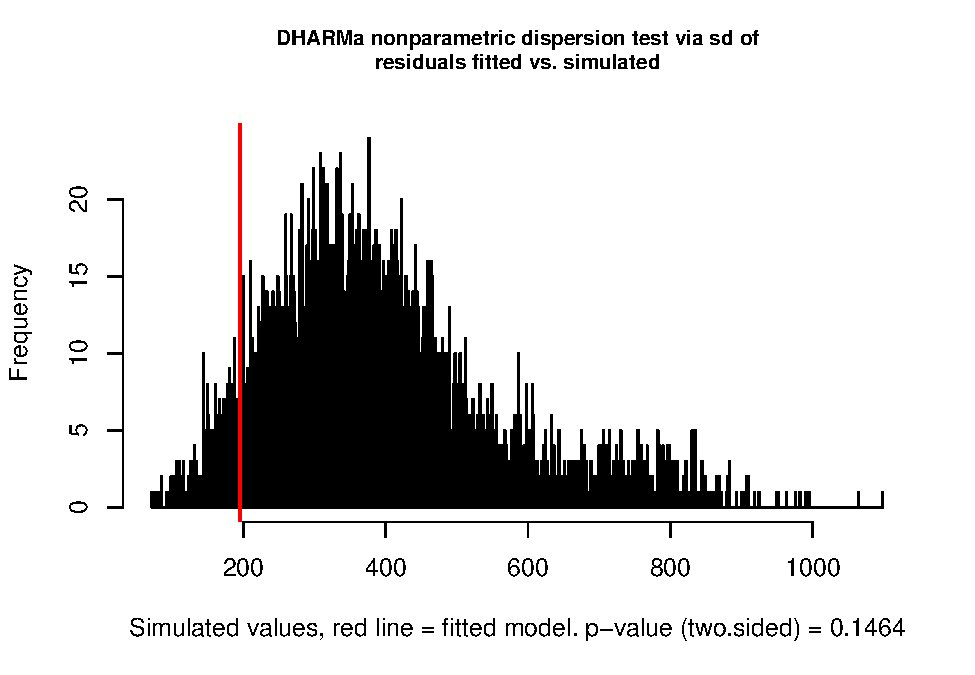
\includegraphics{lathyrus_ms3_3_after_rev_Ecology_files/figure-latex/unnamed-chunk-9-1.pdf}

\begin{Shaded}
\begin{Highlighting}[]
\KeywordTok{plot}\NormalTok{(sim\_path1\_mod2,}\DataTypeTok{quantreg=}\NormalTok{T) }\CommentTok{\# not OK {-} calculate BCA intervals}
\end{Highlighting}
\end{Shaded}

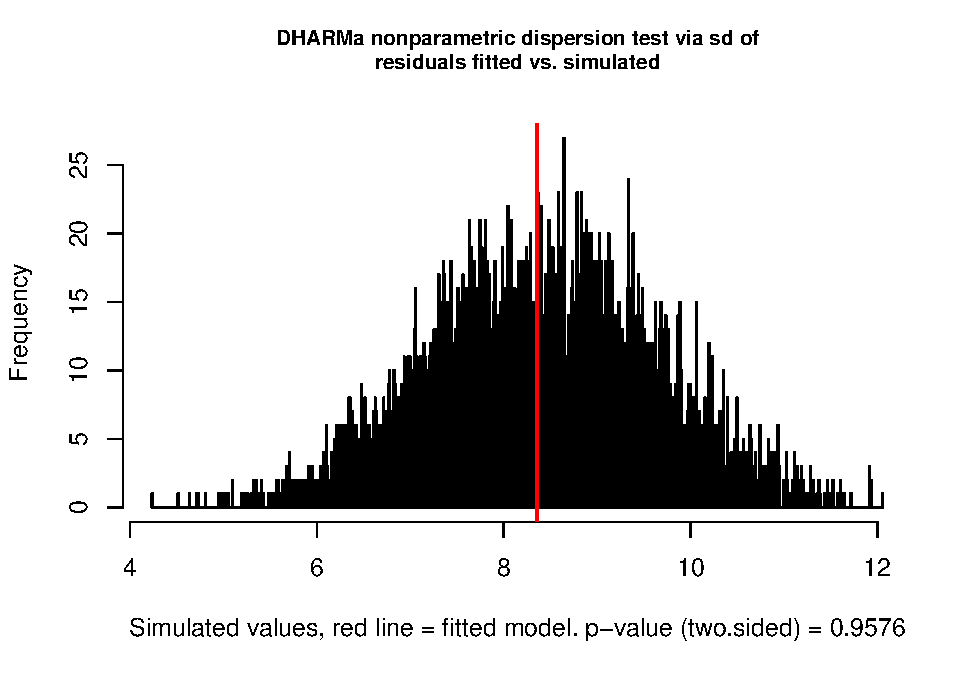
\includegraphics{lathyrus_ms3_3_after_rev_Ecology_files/figure-latex/unnamed-chunk-9-2.pdf}

\begin{Shaded}
\begin{Highlighting}[]
\KeywordTok{plot}\NormalTok{(sim\_path1\_mod3,}\DataTypeTok{quantreg=}\NormalTok{T) }\CommentTok{\# not OK }
\end{Highlighting}
\end{Shaded}

\includegraphics{lathyrus_ms3_3_after_rev_Ecology_files/figure-latex/unnamed-chunk-9-3.pdf}

\begin{Shaded}
\begin{Highlighting}[]
\KeywordTok{plot}\NormalTok{(sim\_path1\_mod4,}\DataTypeTok{quantreg=}\NormalTok{T) }\CommentTok{\# not OK}
\end{Highlighting}
\end{Shaded}

\includegraphics{lathyrus_ms3_3_after_rev_Ecology_files/figure-latex/unnamed-chunk-9-4.pdf}

\begin{Shaded}
\begin{Highlighting}[]
\KeywordTok{testDispersion}\NormalTok{(sim\_path1\_mod3) }\CommentTok{\# OK}
\end{Highlighting}
\end{Shaded}

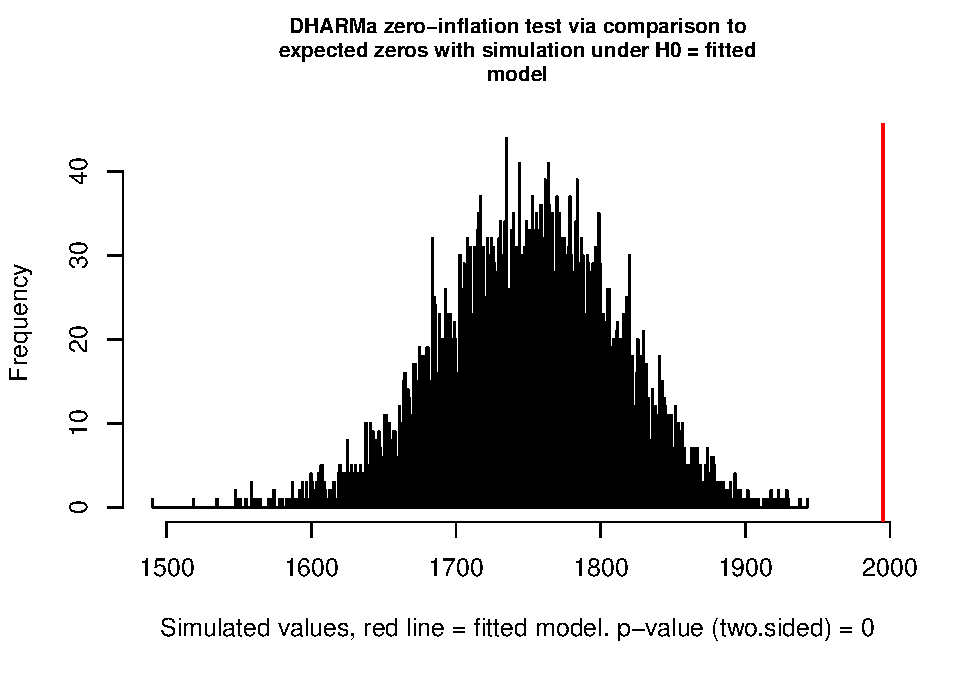
\includegraphics{lathyrus_ms3_3_after_rev_Ecology_files/figure-latex/unnamed-chunk-10-1.pdf}

\begin{verbatim}
## 
##  DHARMa nonparametric dispersion test via sd of residuals fitted vs.
##  simulated
## 
## data:  simulationOutput
## ratioObsSim = 0.50412, p-value = 0.1464
## alternative hypothesis: two.sided
\end{verbatim}

\begin{Shaded}
\begin{Highlighting}[]
\KeywordTok{testDispersion}\NormalTok{(sim\_path1\_mod4) }\CommentTok{\# OK}
\end{Highlighting}
\end{Shaded}

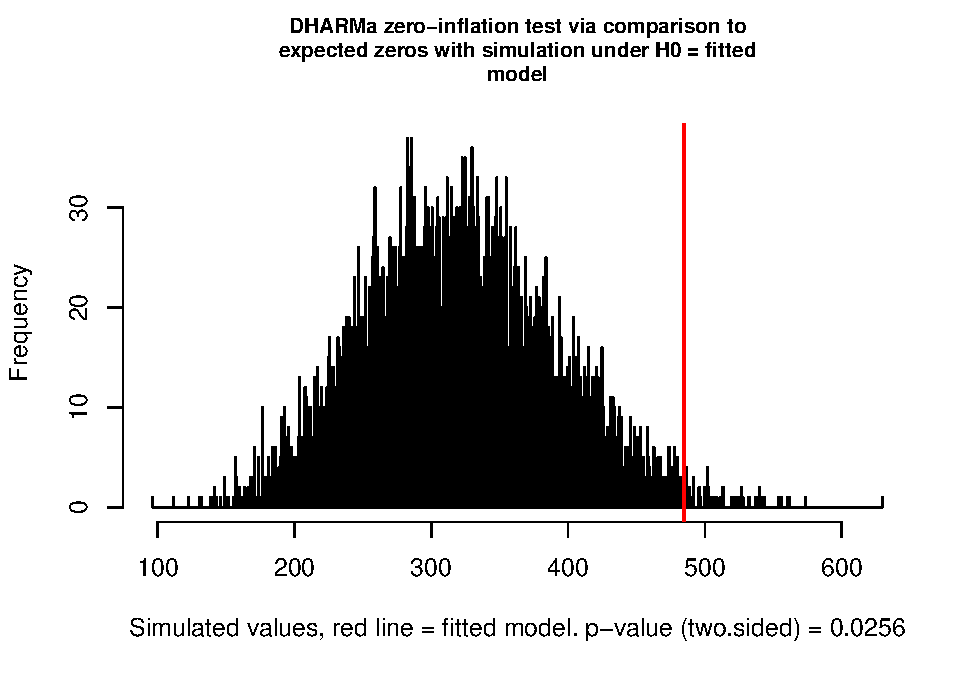
\includegraphics{lathyrus_ms3_3_after_rev_Ecology_files/figure-latex/unnamed-chunk-10-2.pdf}

\begin{verbatim}
## 
##  DHARMa nonparametric dispersion test via sd of residuals fitted vs.
##  simulated
## 
## data:  simulationOutput
## ratioObsSim = 0.99474, p-value = 0.9576
## alternative hypothesis: two.sided
\end{verbatim}

\begin{Shaded}
\begin{Highlighting}[]
\KeywordTok{testZeroInflation}\NormalTok{(sim\_path1\_mod3) }\CommentTok{\# significant}
\end{Highlighting}
\end{Shaded}

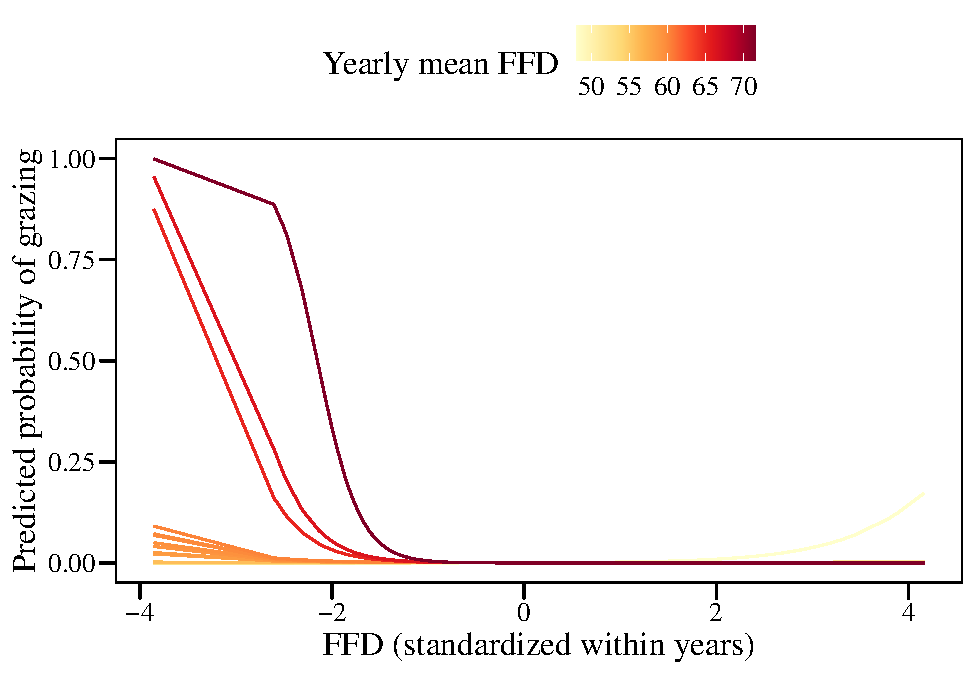
\includegraphics{lathyrus_ms3_3_after_rev_Ecology_files/figure-latex/unnamed-chunk-11-1.pdf}

\begin{verbatim}
## 
##  DHARMa zero-inflation test via comparison to expected zeros with
##  simulation under H0 = fitted model
## 
## data:  simulationOutput
## ratioObsSim = 1.1394, p-value < 2.2e-16
## alternative hypothesis: two.sided
\end{verbatim}

\begin{Shaded}
\begin{Highlighting}[]
\KeywordTok{testZeroInflation}\NormalTok{(sim\_path1\_mod4) }\CommentTok{\# significant}
\end{Highlighting}
\end{Shaded}

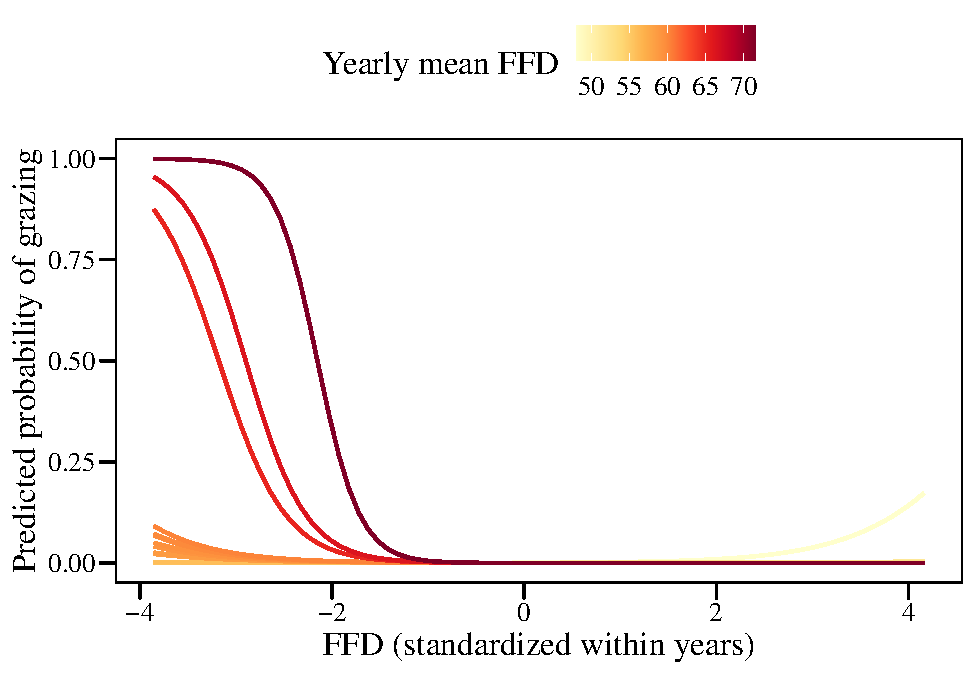
\includegraphics{lathyrus_ms3_3_after_rev_Ecology_files/figure-latex/unnamed-chunk-11-2.pdf}

\begin{verbatim}
## 
##  DHARMa zero-inflation test via comparison to expected zeros with
##  simulation under H0 = fitted model
## 
## data:  simulationOutput
## ratioObsSim = 1.5119, p-value = 0.0256
## alternative hypothesis: two.sided
\end{verbatim}

\hypertarget{refit-models-3-and-4-with-betabinomial-distribution.}{%
\subsection{Refit models 3 and 4 with betabinomial
distribution.}\label{refit-models-3-and-4-with-betabinomial-distribution.}}

\begin{Shaded}
\begin{Highlighting}[]
\NormalTok{path1\_mod3\_bb\textless{}{-}}\KeywordTok{glmmTMB}\NormalTok{(grazing\_corr}\OperatorTok{\textasciitilde{}}\NormalTok{FFD\_s\_y}\OperatorTok{+}\NormalTok{n\_fl\_s\_y}\OperatorTok{+}\NormalTok{(}\DecValTok{1}\OperatorTok{|}\NormalTok{id)}\OperatorTok{+}\NormalTok{(}\DecValTok{1}\OperatorTok{|}\NormalTok{year),}
                            \DataTypeTok{data=}\NormalTok{data\_selag,}\DataTypeTok{family=}\StringTok{"betabinomial"}\NormalTok{,}
                            \DataTypeTok{weights=}\NormalTok{grazing\_weights)}
\NormalTok{path1\_mod4\_bb\textless{}{-}}\KeywordTok{glmmTMB}\NormalTok{(prop\_pred\_seeds}\OperatorTok{\textasciitilde{}}\NormalTok{FFD\_s\_y}\OperatorTok{+}\NormalTok{n\_fl\_s\_y}\OperatorTok{+}\NormalTok{(}\DecValTok{1}\OperatorTok{|}\NormalTok{id)}\OperatorTok{+}\NormalTok{(}\DecValTok{1}\OperatorTok{|}\NormalTok{year),}
                            \DataTypeTok{data=}\NormalTok{data\_selag,}\DataTypeTok{family=}\StringTok{"betabinomial"}\NormalTok{,}
                            \DataTypeTok{weights=}\KeywordTok{round}\NormalTok{(n\_seeds))}
\end{Highlighting}
\end{Shaded}

\hypertarget{model-diagnostics-1}{%
\subsubsection{Model diagnostics}\label{model-diagnostics-1}}

\begin{Shaded}
\begin{Highlighting}[]
\NormalTok{sim\_path1\_mod3\_bb \textless{}{-}}\StringTok{ }\KeywordTok{simulateResiduals}\NormalTok{(}\DataTypeTok{fittedModel =}\NormalTok{ path1\_mod3\_bb, }\DataTypeTok{n =} \DecValTok{5000}\NormalTok{) }
\NormalTok{sim\_path1\_mod4\_bb \textless{}{-}}\StringTok{ }\KeywordTok{simulateResiduals}\NormalTok{(}\DataTypeTok{fittedModel =}\NormalTok{ path1\_mod4\_bb, }\DataTypeTok{n =} \DecValTok{5000}\NormalTok{) }
\end{Highlighting}
\end{Shaded}

qq-plot and plot of residuals vs.~predicted:

\begin{Shaded}
\begin{Highlighting}[]
\KeywordTok{plot}\NormalTok{(sim\_path1\_mod3\_bb,}\DataTypeTok{quantreg=}\NormalTok{T) }\CommentTok{\# not OK }
\end{Highlighting}
\end{Shaded}

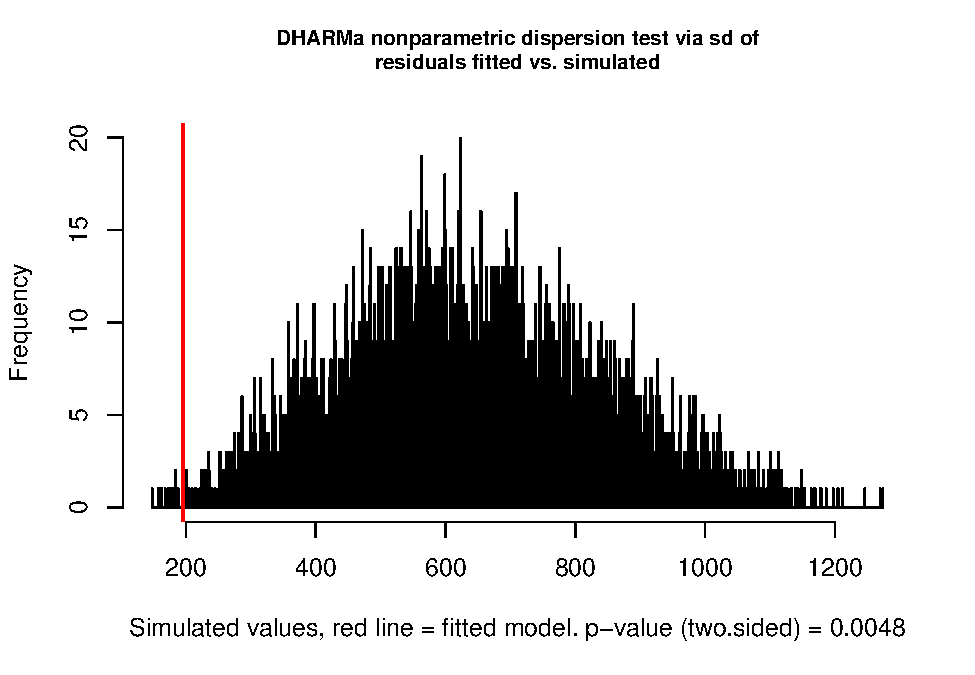
\includegraphics{lathyrus_ms3_3_after_rev_Ecology_files/figure-latex/unnamed-chunk-14-1.pdf}

\begin{Shaded}
\begin{Highlighting}[]
\KeywordTok{plot}\NormalTok{(sim\_path1\_mod4\_bb,}\DataTypeTok{quantreg=}\NormalTok{T) }\CommentTok{\# not OK}
\end{Highlighting}
\end{Shaded}

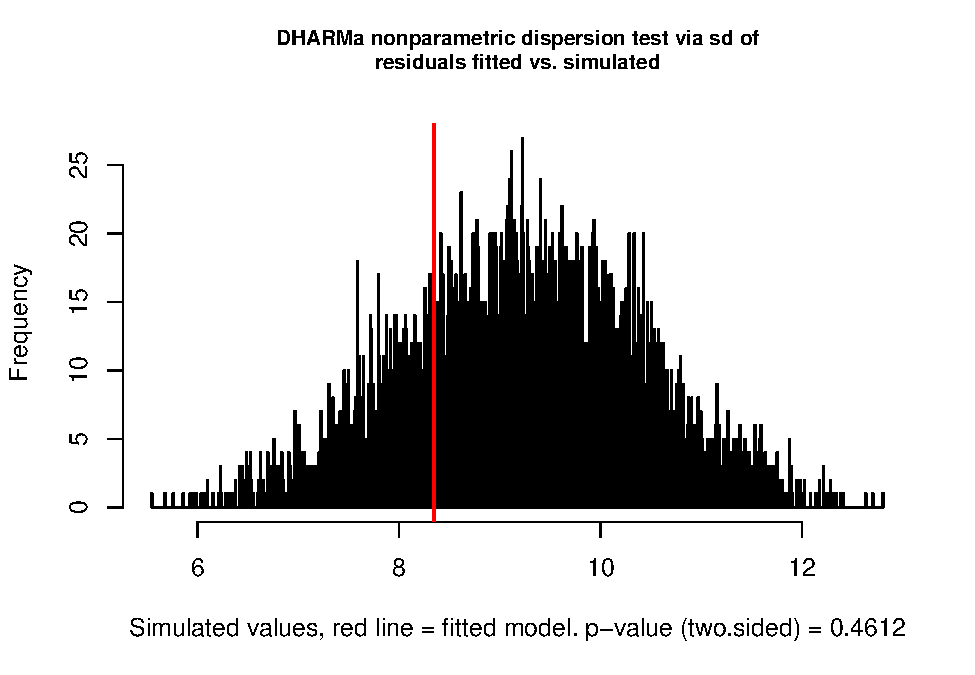
\includegraphics{lathyrus_ms3_3_after_rev_Ecology_files/figure-latex/unnamed-chunk-14-2.pdf}

KS test being significant is probably not a problem.

From \url{https://github.com/florianhartig/DHARMa/issues/181}

"the p-value shows you that there is a significant deviation from the
assumed distribution, but significance != effect size. In other words,
if you have a large number of data points (as you have here), even the
slightest deviation will become significant. {[}\ldots{]} the qq-plot is
nearly linear, suggesting that the overall distribution is roughly OK.

\begin{Shaded}
\begin{Highlighting}[]
\KeywordTok{testDispersion}\NormalTok{(sim\_path1\_mod3\_bb) }\CommentTok{\# a bit of underdispersion, probably OK}
\end{Highlighting}
\end{Shaded}

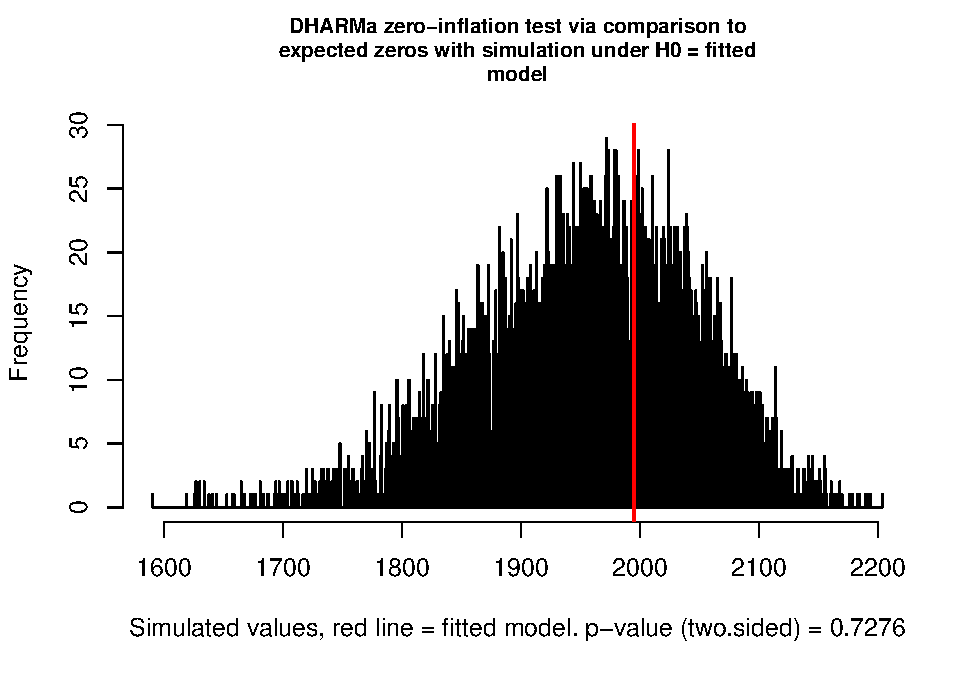
\includegraphics{lathyrus_ms3_3_after_rev_Ecology_files/figure-latex/unnamed-chunk-15-1.pdf}

\begin{verbatim}
## 
##  DHARMa nonparametric dispersion test via sd of residuals fitted vs.
##  simulated
## 
## data:  simulationOutput
## ratioObsSim = 0.30572, p-value = 0.0048
## alternative hypothesis: two.sided
\end{verbatim}

\begin{Shaded}
\begin{Highlighting}[]
\KeywordTok{testDispersion}\NormalTok{(sim\_path1\_mod4\_bb) }\CommentTok{\# OK}
\end{Highlighting}
\end{Shaded}

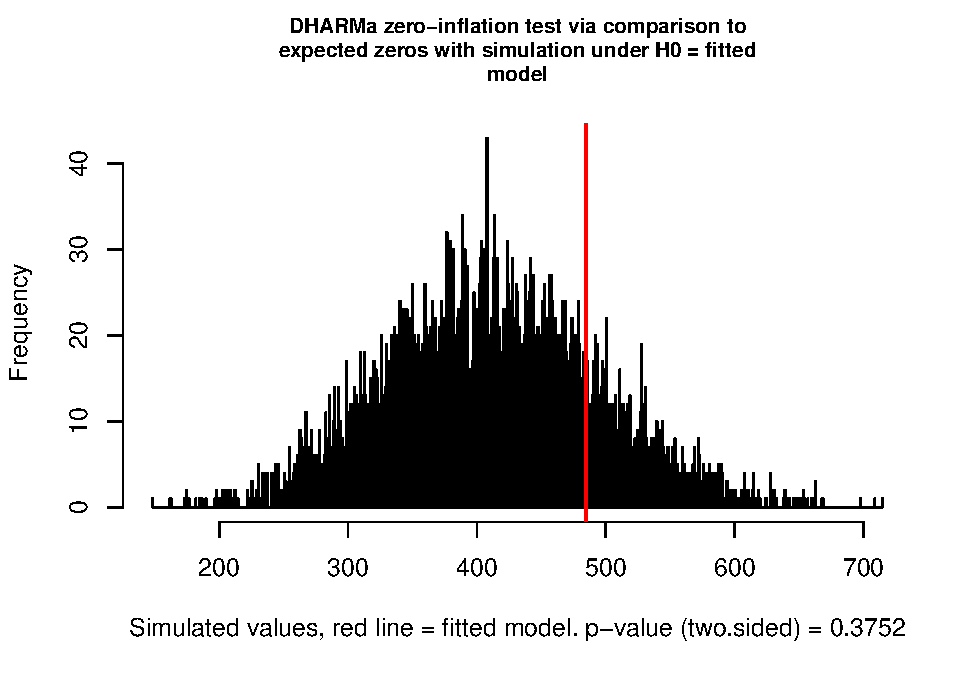
\includegraphics{lathyrus_ms3_3_after_rev_Ecology_files/figure-latex/unnamed-chunk-15-2.pdf}

\begin{verbatim}
## 
##  DHARMa nonparametric dispersion test via sd of residuals fitted vs.
##  simulated
## 
## data:  simulationOutput
## ratioObsSim = 0.90432, p-value = 0.4612
## alternative hypothesis: two.sided
\end{verbatim}

\begin{Shaded}
\begin{Highlighting}[]
\KeywordTok{testZeroInflation}\NormalTok{(sim\_path1\_mod3\_bb) }\CommentTok{\# OK}
\end{Highlighting}
\end{Shaded}

\includegraphics{lathyrus_ms3_3_after_rev_Ecology_files/figure-latex/unnamed-chunk-16-1.pdf}

\begin{verbatim}
## 
##  DHARMa zero-inflation test via comparison to expected zeros with
##  simulation under H0 = fitted model
## 
## data:  simulationOutput
## ratioObsSim = 1.0197, p-value = 0.7276
## alternative hypothesis: two.sided
\end{verbatim}

\begin{Shaded}
\begin{Highlighting}[]
\KeywordTok{testZeroInflation}\NormalTok{(sim\_path1\_mod4\_bb) }\CommentTok{\# OK}
\end{Highlighting}
\end{Shaded}

\includegraphics{lathyrus_ms3_3_after_rev_Ecology_files/figure-latex/unnamed-chunk-16-2.pdf}

\begin{verbatim}
## 
##  DHARMa zero-inflation test via comparison to expected zeros with
##  simulation under H0 = fitted model
## 
## data:  simulationOutput
## ratioObsSim = 1.1793, p-value = 0.3752
## alternative hypothesis: two.sided
\end{verbatim}

\begin{Shaded}
\begin{Highlighting}[]
\KeywordTok{anova}\NormalTok{(path1\_mod3,path1\_mod3\_bb)}
\end{Highlighting}
\end{Shaded}

\begin{verbatim}
## Data: data_selag
## Models:
## path1_mod3: grazing_corr ~ FFD_s_y + n_fl_s_y + (1 | id) + (1 | year), zi=~0, disp=~1
## path1_mod3_bb: grazing_corr ~ FFD_s_y + n_fl_s_y + (1 | id) + (1 | year), zi=~0, disp=~1
##               Df    AIC    BIC logLik deviance  Chisq Chi Df Pr(>Chisq)    
## path1_mod3     5 155103 155132 -77547   155093                             
## path1_mod3_bb  6   3601   3636  -1795     3589 151504      1  < 2.2e-16 ***
## ---
## Signif. codes:  0 '***' 0.001 '**' 0.01 '*' 0.05 '.' 0.1 ' ' 1
\end{verbatim}

\begin{Shaded}
\begin{Highlighting}[]
\KeywordTok{anova}\NormalTok{(path1\_mod4,path1\_mod4\_bb)}
\end{Highlighting}
\end{Shaded}

\begin{verbatim}
## Data: data_selag
## Models:
## path1_mod4: prop_pred_seeds ~ FFD_s_y + n_fl_s_y + (1 | id) + (1 | year), zi=~0, disp=~1
## path1_mod4_bb: prop_pred_seeds ~ FFD_s_y + n_fl_s_y + (1 | id) + (1 | year), zi=~0, disp=~1
##               Df    AIC    BIC  logLik deviance  Chisq Chi Df Pr(>Chisq)    
## path1_mod4     5 6696.0 6721.8 -3343.0   6686.0                             
## path1_mod4_bb  6 4953.5 4984.4 -2470.8   4941.5 1744.5      1  < 2.2e-16 ***
## ---
## Signif. codes:  0 '***' 0.001 '**' 0.01 '*' 0.05 '.' 0.1 ' ' 1
\end{verbatim}

\begin{Shaded}
\begin{Highlighting}[]
\KeywordTok{AIC}\NormalTok{(path1\_mod3,path1\_mod3\_bb)}
\end{Highlighting}
\end{Shaded}

\begin{verbatim}
##               df        AIC
## path1_mod3     5 155103.361
## path1_mod3_bb  6   3601.166
\end{verbatim}

\begin{Shaded}
\begin{Highlighting}[]
\KeywordTok{AIC}\NormalTok{(path1\_mod4,path1\_mod4\_bb)}
\end{Highlighting}
\end{Shaded}

\begin{verbatim}
##               df      AIC
## path1_mod4     5 6695.992
## path1_mod4_bb  6 4953.500
\end{verbatim}

Use betabinomial models.

Tested quadratic effects of FFD on grazing and seed predation, and they
were not significant in betabinomial models.

\hypertarget{boostrapped-confidence-intervals-for-model-2}{%
\subsection{Boostrapped confidence intervals for model
2:}\label{boostrapped-confidence-intervals-for-model-2}}

\hypertarget{mixed-model}{%
\subsubsection{Mixed model}\label{mixed-model}}

\begin{Shaded}
\begin{Highlighting}[]
\NormalTok{path1\_mod2\_glmer\textless{}{-}}\KeywordTok{glmer}\NormalTok{(fitness\_rel\_y}\OperatorTok{\textasciitilde{}}\NormalTok{FFD\_s\_y}\OperatorTok{+}\NormalTok{n\_fl\_s\_y}\OperatorTok{+}\NormalTok{grazing\_corr}\OperatorTok{+}
\StringTok{                          }\NormalTok{prop\_pred\_seeds}\OperatorTok{+}\NormalTok{(}\DecValTok{1}\OperatorTok{|}\NormalTok{id)}\OperatorTok{+}\NormalTok{(}\DecValTok{1}\OperatorTok{|}\NormalTok{year),}\DataTypeTok{data=}\NormalTok{data\_selag)}
\CommentTok{\# We need to use glmer for this}
\end{Highlighting}
\end{Shaded}

\begin{Shaded}
\begin{Highlighting}[]
\KeywordTok{confint}\NormalTok{(b\_par\_}\DecValTok{1}\NormalTok{,}\DataTypeTok{level=}\FloatTok{0.95}\NormalTok{, }\DataTypeTok{method=}\StringTok{"boot"}\NormalTok{) }\CommentTok{\# Percentile method}
\end{Highlighting}
\end{Shaded}

\begin{verbatim}
##                      2.5 %      97.5 %
## (Intercept)      2.3664280  5.93437756
## FFD_s_y         -0.3156583 -0.04331491
## n_fl_s_y         0.4743067  0.69936623
## grazing_corr    -2.1922090 -0.53065021
## prop_pred_seeds -4.0396053 -3.24794402
\end{verbatim}

Similar to significances in the lmer model.

\hypertarget{lm-elsas-code-not-used}{%
\subsubsection{LM (Elsa's code) (not
used)}\label{lm-elsas-code-not-used}}

Similar to significances in the lmer model except for grazing, where the
CIs overlap zero here. Use only percentile method?

\hypertarget{new-path-model}{%
\subsection{New path model}\label{new-path-model}}

\begin{Shaded}
\begin{Highlighting}[]
\KeywordTok{summary}\NormalTok{(path1\_mod1)}\OperatorTok{$}\NormalTok{coefficients }
\end{Highlighting}
\end{Shaded}

\begin{verbatim}
## $cond
##                Estimate Std. Error    z value     Pr(>|z|)
## (Intercept)   0.5448470 0.21257583   2.563071 1.037508e-02
## FFD_s_y      -0.6968366 0.06747741 -10.326961 5.321988e-25
## n_fl_s_y      0.6111297 0.07683091   7.954216 1.802689e-15
## grazing_corr -3.8250266 0.32225988 -11.869385 1.707182e-32
## 
## $zi
## NULL
## 
## $disp
## NULL
\end{verbatim}

\begin{Shaded}
\begin{Highlighting}[]
\CommentTok{\# std coefs if needed from path1 without random effects}
\KeywordTok{summary}\NormalTok{(path1\_mod2)}\OperatorTok{$}\NormalTok{coefficients }
\end{Highlighting}
\end{Shaded}

\begin{verbatim}
## $cond
##                   Estimate Std. Error    z value     Pr(>|z|)
## (Intercept)      4.1866333 0.88694757   4.720271 2.355301e-06
## FFD_s_y         -0.1790698 0.06873317  -2.605290 9.179656e-03
## n_fl_s_y         0.5868972 0.05766612  10.177505 2.498870e-24
## grazing_corr    -1.3597652 0.42561090  -3.194855 1.399010e-03
## prop_pred_seeds -3.6442115 0.20386754 -17.875388 1.833937e-71
## 
## $zi
## NULL
## 
## $disp
## NULL
\end{verbatim}

\begin{Shaded}
\begin{Highlighting}[]
\CommentTok{\# get significances from bootstrapped CIs, std coefs from path1 without random effects}
\KeywordTok{summary}\NormalTok{(path1\_mod3\_bb)}\OperatorTok{$}\NormalTok{coefficients }
\end{Highlighting}
\end{Shaded}

\begin{verbatim}
## $cond
##               Estimate Std. Error   z value     Pr(>|z|)
## (Intercept) -2.9368887 0.32909846 -8.924043 4.495707e-19
## FFD_s_y     -0.3479031 0.08335881 -4.173561 2.998753e-05
## n_fl_s_y     0.1875620 0.06457848  2.904404 3.679536e-03
## 
## $zi
## NULL
## 
## $disp
## NULL
\end{verbatim}

\begin{Shaded}
\begin{Highlighting}[]
\CommentTok{\# significances and ustd coefs from here, std if needed from path1 without random effects}
\KeywordTok{summary}\NormalTok{(path1\_mod4\_bb)}\OperatorTok{$}\NormalTok{coefficients }
\end{Highlighting}
\end{Shaded}

\begin{verbatim}
## $cond
##               Estimate Std. Error   z value     Pr(>|z|)
## (Intercept) -0.7491371 0.31175650 -2.402956 1.626315e-02
## FFD_s_y      0.1007740 0.05463502  1.844495 6.511103e-02
## n_fl_s_y     0.2060346 0.04261941  4.834291 1.336212e-06
## 
## $zi
## NULL
## 
## $disp
## NULL
\end{verbatim}

\begin{Shaded}
\begin{Highlighting}[]
\CommentTok{\# significances and ustd coefs from here, std if needed from path1 without random effects}
\end{Highlighting}
\end{Shaded}

piecewiseSEM does not work with glmmTMB - and that is the only package I
found that fits betabinomial mixed models.

\begin{Shaded}
\begin{Highlighting}[]
\NormalTok{path1\_norandom\textless{}{-}}\KeywordTok{psem}\NormalTok{(}
  \KeywordTok{glm}\NormalTok{(seeds\_}\DecValTok{01}\OperatorTok{\textasciitilde{}}\NormalTok{FFD\_s\_y}\OperatorTok{+}\NormalTok{n\_fl\_s\_y}\OperatorTok{+}\NormalTok{grazing\_corr,}
                \DataTypeTok{data=}\NormalTok{data\_selag,}\DataTypeTok{family=}\StringTok{"binomial"}\NormalTok{),}
  \KeywordTok{lm}\NormalTok{(fitness\_rel\_y}\OperatorTok{\textasciitilde{}}\NormalTok{FFD\_s\_y}\OperatorTok{+}\NormalTok{n\_fl\_s\_y}\OperatorTok{+}\NormalTok{grazing\_corr}\OperatorTok{+}\NormalTok{prop\_pred\_seeds,}
               \DataTypeTok{data=}\NormalTok{data\_selag),}
  \KeywordTok{glm}\NormalTok{(grazing\_corr}\OperatorTok{\textasciitilde{}}\NormalTok{FFD\_s\_y}\OperatorTok{+}\NormalTok{n\_fl\_s\_y,}
                  \DataTypeTok{data=}\NormalTok{data\_selag,}\DataTypeTok{family=}\StringTok{"binomial"}\NormalTok{,}\DataTypeTok{weights=}\NormalTok{grazing\_weights),}
  \KeywordTok{glm}\NormalTok{(prop\_pred\_seeds}\OperatorTok{\textasciitilde{}}\NormalTok{FFD\_s\_y}\OperatorTok{+}\NormalTok{n\_fl\_s\_y,}
                  \DataTypeTok{data=}\NormalTok{data\_selag,}\DataTypeTok{family=}\StringTok{"binomial"}\NormalTok{,}
                  \DataTypeTok{weights=}\NormalTok{n\_seeds))}
\KeywordTok{coefs}\NormalTok{(path1\_norandom) }
\end{Highlighting}
\end{Shaded}

\begin{verbatim}
##           Response       Predictor Estimate Std.Error   DF Crit.Value P.Value
## 1         seeds_01         FFD_s_y  -0.6041    0.0559 2372   -10.8057  0.0000
## 2         seeds_01        n_fl_s_y   0.4999    0.0642 2372     7.7907  0.0000
## 3         seeds_01    grazing_corr  -3.2497    0.2395 2372   -13.5712  0.0000
## 4    fitness_rel_y         FFD_s_y  -0.2054    0.0881 1276    -2.3322  0.0198
## 5    fitness_rel_y        n_fl_s_y   0.4506    0.0726 1276     6.2070  0.0000
## 6    fitness_rel_y    grazing_corr   0.6428    0.5272 1276     1.2192  0.2230
## 7    fitness_rel_y prop_pred_seeds  -1.6647    0.1931 1276    -8.6187  0.0000
## 8     grazing_corr         FFD_s_y  -0.1169    0.0054 2350   -21.5365  0.0000
## 9     grazing_corr        n_fl_s_y  -0.0692    0.0033 2350   -20.7038  0.0000
## 10 prop_pred_seeds         FFD_s_y  -0.0330    0.0208 1278    -1.5837  0.1133
## 11 prop_pred_seeds        n_fl_s_y   0.0893    0.0120 1278     7.4500  0.0000
##    Std.Estimate    
## 1       -0.2741 ***
## 2        0.2268 ***
## 3       -0.4572 ***
## 4       -0.0965   *
## 5        0.2118 ***
## 6        0.0937    
## 7       -0.2859 ***
## 8       -0.0641 ***
## 9       -0.0379 ***
## 10      -0.0181    
## 11       0.0490 ***
\end{verbatim}

\begin{Shaded}
\begin{Highlighting}[]
\KeywordTok{plot}\NormalTok{(path1\_norandom)}
\end{Highlighting}
\end{Shaded}

Figure 1: Path diagram (made in Inkscape)

\% of grazed plants that produced seeds

\begin{Shaded}
\begin{Highlighting}[]
\KeywordTok{nrow}\NormalTok{(}\KeywordTok{subset}\NormalTok{(data\_selag,grazing\_corr}\OperatorTok{\textgreater{}}\DecValTok{0}\OperatorTok{\&}\NormalTok{n\_seeds}\OperatorTok{\textgreater{}}\DecValTok{0}\NormalTok{))}\OperatorTok{*}\DecValTok{100}\OperatorTok{/}
\StringTok{  }\KeywordTok{nrow}\NormalTok{(}\KeywordTok{subset}\NormalTok{(data\_selag,grazing\_corr}\OperatorTok{\textgreater{}}\DecValTok{0}\NormalTok{))}
\end{Highlighting}
\end{Shaded}

\begin{verbatim}
## [1] 28.63341
\end{verbatim}

\% of plants with more than half of their above-ground structures
removed that produced seeds

\begin{Shaded}
\begin{Highlighting}[]
\KeywordTok{nrow}\NormalTok{(}\KeywordTok{subset}\NormalTok{(data\_selag,grazing\_corr}\OperatorTok{\textgreater{}}\FloatTok{0.5}\OperatorTok{\&}\NormalTok{n\_seeds}\OperatorTok{\textgreater{}}\DecValTok{0}\NormalTok{))}\OperatorTok{*}\DecValTok{100}\OperatorTok{/}
\StringTok{  }\KeywordTok{nrow}\NormalTok{(}\KeywordTok{subset}\NormalTok{(data\_selag,grazing\_corr}\OperatorTok{\textgreater{}}\DecValTok{0}\NormalTok{))}
\end{Highlighting}
\end{Shaded}

\begin{verbatim}
## [1] 6.290672
\end{verbatim}

Only 29\% of plants that experienced any grazing produced seeds, and 6\%
of plants that had more than half of their above-ground structures
removed.

\hypertarget{h3}{%
\section{H3}\label{h3}}

H3: Variation in climatic conditions during spring among years causes
differences in selection on flowering time, through effects mediated by
the intensity of biotic interactions.

\hypertarget{h3---part-1}{%
\section{H3 - Part 1}\label{h3---part-1}}

Variation in climatic conditions during spring among years influences
the intensity of biotic interactions and the covariance between
interaction intensity and plant phenology.

First, models to test the effect of spring temperatures on antagonistic
interactions, while accounting for FFD and number of flowers. Using FFD
and number of flowers standardized within years, temperatures
standardized across years. Including interactions among FFD and
temperatures. NOT including a random effect of year because there is
only one value of temperature for each year.

\hypertarget{grazing}{%
\subsection{Grazing}\label{grazing}}

\begin{Shaded}
\begin{Highlighting}[]
\NormalTok{mod\_grazing\textless{}{-}}\KeywordTok{glmmTMB}\NormalTok{(}\KeywordTok{cbind}\NormalTok{(grazing\_success,grazing\_failure)}\OperatorTok{\textasciitilde{}}
\StringTok{                     }\NormalTok{(}\KeywordTok{scale}\NormalTok{(mean\_}\DecValTok{3}\NormalTok{)}\OperatorTok{+}\KeywordTok{scale}\NormalTok{(mean\_}\DecValTok{4}\NormalTok{)}\OperatorTok{+}\KeywordTok{scale}\NormalTok{(mean\_}\DecValTok{5}\NormalTok{))}\OperatorTok{*}\NormalTok{FFD\_s\_y}\OperatorTok{+}
\StringTok{                     }\NormalTok{n\_fl\_s\_y}\OperatorTok{+}\NormalTok{(}\DecValTok{1}\OperatorTok{|}\NormalTok{id),}\DataTypeTok{data =}\NormalTok{ data\_selag,}
                   \DataTypeTok{family=}\StringTok{"binomial"}\NormalTok{)}
\KeywordTok{summary}\NormalTok{(mod\_grazing)}
\end{Highlighting}
\end{Shaded}

\begin{verbatim}
##  Family: binomial  ( logit )
## Formula:          
## cbind(grazing_success, grazing_failure) ~ (scale(mean_3) + scale(mean_4) +  
##     scale(mean_5)) * FFD_s_y + n_fl_s_y + (1 | id)
## Data: data_selag
## 
##      AIC      BIC   logLik deviance df.resid 
## 174950.7 175008.3 -87465.4 174930.7     2344 
## 
## Random effects:
## 
## Conditional model:
##  Groups Name        Variance Std.Dev.
##  id     (Intercept) 48.66    6.976   
## Number of obs: 2354, groups:  id, 834
## 
## Conditional model:
##                        Estimate Std. Error z value Pr(>|z|)    
## (Intercept)           -8.990310   0.459323  -19.57  < 2e-16 ***
## scale(mean_3)          0.683845   0.007932   86.21  < 2e-16 ***
## scale(mean_4)          0.022606   0.005433    4.16 3.17e-05 ***
## scale(mean_5)         -0.066343   0.028336   -2.34   0.0192 *  
## FFD_s_y               -0.942016   0.015389  -61.22  < 2e-16 ***
## n_fl_s_y              -0.182051   0.005101  -35.69  < 2e-16 ***
## scale(mean_3):FFD_s_y  0.522687   0.008510   61.42  < 2e-16 ***
## scale(mean_4):FFD_s_y  0.168588   0.005916   28.50  < 2e-16 ***
## scale(mean_5):FFD_s_y  1.788498   0.031905   56.06  < 2e-16 ***
## ---
## Signif. codes:  0 '***' 0.001 '**' 0.01 '*' 0.05 '.' 0.1 ' ' 1
\end{verbatim}

\hypertarget{model-diagnostics-2}{%
\subsubsection{Model diagnostics}\label{model-diagnostics-2}}

Simulate residuals of the model:

\begin{Shaded}
\begin{Highlighting}[]
\NormalTok{sim\_mod\_grazing \textless{}{-}}\StringTok{ }\KeywordTok{simulateResiduals}\NormalTok{(}\DataTypeTok{fittedModel=}\NormalTok{mod\_grazing,}\DataTypeTok{n=}\DecValTok{5000}\NormalTok{)}
\end{Highlighting}
\end{Shaded}

qq-plot and plot of residuals vs.~predicted:

\begin{Shaded}
\begin{Highlighting}[]
\KeywordTok{plot}\NormalTok{(sim\_mod\_grazing,}\DataTypeTok{quantreg=}\NormalTok{T)}
\end{Highlighting}
\end{Shaded}

\includegraphics{lathyrus_ms3_3_after_rev_Ecology_files/figure-latex/unnamed-chunk-28-1.pdf}

\begin{Shaded}
\begin{Highlighting}[]
\KeywordTok{testDispersion}\NormalTok{(sim\_mod\_grazing)}
\end{Highlighting}
\end{Shaded}

\includegraphics{lathyrus_ms3_3_after_rev_Ecology_files/figure-latex/unnamed-chunk-29-1.pdf}

\begin{verbatim}
## 
##  DHARMa nonparametric dispersion test via sd of residuals fitted vs.
##  simulated
## 
## data:  simulationOutput
## ratioObsSim = 0.41949, p-value = 0.026
## alternative hypothesis: two.sided
\end{verbatim}

Slightly underdispersed.

\begin{Shaded}
\begin{Highlighting}[]
\KeywordTok{testZeroInflation}\NormalTok{(sim\_mod\_grazing)}
\end{Highlighting}
\end{Shaded}

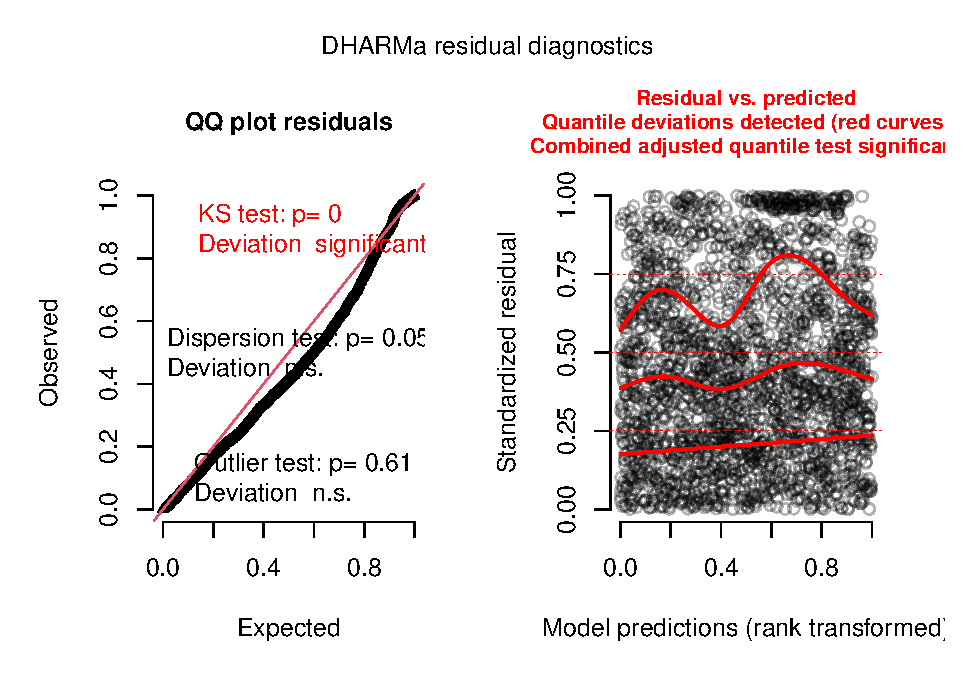
\includegraphics{lathyrus_ms3_3_after_rev_Ecology_files/figure-latex/unnamed-chunk-30-1.pdf}

\begin{verbatim}
## 
##  DHARMa zero-inflation test via comparison to expected zeros with
##  simulation under H0 = fitted model
## 
## data:  simulationOutput
## ratioObsSim = 1.1381, p-value < 2.2e-16
## alternative hypothesis: two.sided
\end{verbatim}

Test of zero inflation is significant.

\hypertarget{try-with-betabinomial}{%
\subsubsection{Try with betabinomial}\label{try-with-betabinomial}}

\begin{Shaded}
\begin{Highlighting}[]
\NormalTok{mod\_grazing\_bb\textless{}{-}}\KeywordTok{glmmTMB}\NormalTok{(}\KeywordTok{cbind}\NormalTok{(grazing\_success,grazing\_failure)}\OperatorTok{\textasciitilde{}}
\StringTok{                       }\NormalTok{(}\KeywordTok{scale}\NormalTok{(mean\_}\DecValTok{3}\NormalTok{)}\OperatorTok{+}\KeywordTok{scale}\NormalTok{(mean\_}\DecValTok{4}\NormalTok{)}\OperatorTok{+}\KeywordTok{scale}\NormalTok{(mean\_}\DecValTok{5}\NormalTok{))}\OperatorTok{*}\NormalTok{FFD\_s\_y}\OperatorTok{+}
\StringTok{                       }\NormalTok{n\_fl\_s\_y}\OperatorTok{+}\NormalTok{(}\DecValTok{1}\OperatorTok{|}\NormalTok{id),}\DataTypeTok{data =}\NormalTok{ data\_selag,}
                     \DataTypeTok{family=}\StringTok{"betabinomial"}\NormalTok{)}
\KeywordTok{summary}\NormalTok{(mod\_grazing\_bb)}
\end{Highlighting}
\end{Shaded}

\begin{verbatim}
##  Family: betabinomial  ( logit )
## Formula:          
## cbind(grazing_success, grazing_failure) ~ (scale(mean_3) + scale(mean_4) +  
##     scale(mean_5)) * FFD_s_y + n_fl_s_y + (1 | id)
## Data: data_selag
## 
##      AIC      BIC   logLik deviance df.resid 
##   4013.7   4077.1  -1995.8   3991.7     2343 
## 
## Random effects:
## 
## Conditional model:
##  Groups Name        Variance Std.Dev.
##  id     (Intercept) 0.2367   0.4865  
## Number of obs: 2354, groups:  id, 834
## 
## Overdispersion parameter for betabinomial family (): 0.141 
## 
## Conditional model:
##                       Estimate Std. Error z value Pr(>|z|)    
## (Intercept)           -2.23190    0.09050 -24.663  < 2e-16 ***
## scale(mean_3)          0.50384    0.06704   7.516 5.66e-14 ***
## scale(mean_4)         -0.33282    0.06416  -5.187 2.14e-07 ***
## scale(mean_5)         -0.44010    0.08623  -5.104 3.32e-07 ***
## FFD_s_y               -0.25577    0.07307  -3.500 0.000464 ***
## n_fl_s_y               0.15921    0.05901   2.698 0.006976 ** 
## scale(mean_3):FFD_s_y  0.10707    0.07179   1.491 0.135832    
## scale(mean_4):FFD_s_y -0.12757    0.06553  -1.947 0.051571 .  
## scale(mean_5):FFD_s_y  0.02182    0.08916   0.245 0.806639    
## ---
## Signif. codes:  0 '***' 0.001 '**' 0.01 '*' 0.05 '.' 0.1 ' ' 1
\end{verbatim}

\hypertarget{model-diagnostics-3}{%
\subsubsection{Model diagnostics}\label{model-diagnostics-3}}

Simulate residuals of the model:

\begin{Shaded}
\begin{Highlighting}[]
\NormalTok{sim\_mod\_grazing\_bb \textless{}{-}}\StringTok{ }\KeywordTok{simulateResiduals}\NormalTok{(}\DataTypeTok{fittedModel=}\NormalTok{mod\_grazing\_bb,}\DataTypeTok{n=}\DecValTok{5000}\NormalTok{)}
\end{Highlighting}
\end{Shaded}

qq-plot and plot of residuals vs.~predicted:

\begin{Shaded}
\begin{Highlighting}[]
\KeywordTok{plot}\NormalTok{(sim\_mod\_grazing\_bb,}\DataTypeTok{quantreg=}\NormalTok{T)}
\end{Highlighting}
\end{Shaded}

\includegraphics{lathyrus_ms3_3_after_rev_Ecology_files/figure-latex/unnamed-chunk-33-1.pdf}

\begin{Shaded}
\begin{Highlighting}[]
\KeywordTok{testDispersion}\NormalTok{(sim\_mod\_grazing\_bb)}
\end{Highlighting}
\end{Shaded}

\includegraphics{lathyrus_ms3_3_after_rev_Ecology_files/figure-latex/unnamed-chunk-34-1.pdf}

\begin{verbatim}
## 
##  DHARMa nonparametric dispersion test via sd of residuals fitted vs.
##  simulated
## 
## data:  simulationOutput
## ratioObsSim = 0.32727, p-value < 2.2e-16
## alternative hypothesis: two.sided
\end{verbatim}

Still underdispersion.

\begin{Shaded}
\begin{Highlighting}[]
\KeywordTok{testZeroInflation}\NormalTok{(sim\_mod\_grazing\_bb)}
\end{Highlighting}
\end{Shaded}

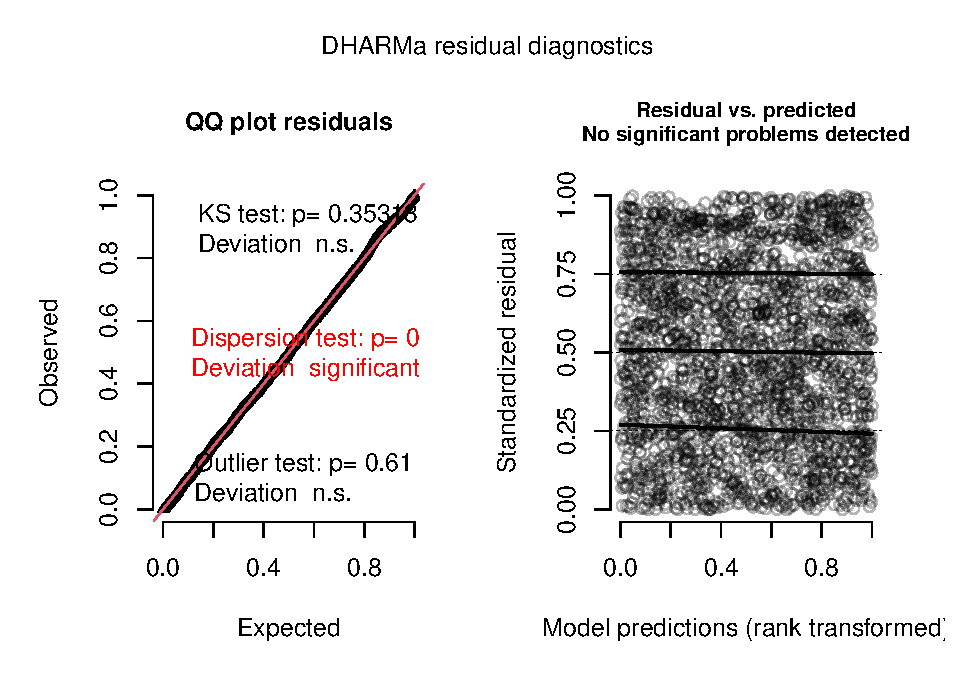
\includegraphics{lathyrus_ms3_3_after_rev_Ecology_files/figure-latex/unnamed-chunk-35-1.pdf}

\begin{verbatim}
## 
##  DHARMa zero-inflation test via comparison to expected zeros with
##  simulation under H0 = fitted model
## 
## data:  simulationOutput
## ratioObsSim = 0.9984, p-value = 0.8616
## alternative hypothesis: two.sided
\end{verbatim}

But zero inflation is fixed

\begin{Shaded}
\begin{Highlighting}[]
\KeywordTok{anova}\NormalTok{(mod\_grazing,mod\_grazing\_bb)}
\end{Highlighting}
\end{Shaded}

\begin{verbatim}
## Data: data_selag
## Models:
## mod_grazing: cbind(grazing_success, grazing_failure) ~ (scale(mean_3) + scale(mean_4) + , zi=~0, disp=~1
## mod_grazing:     scale(mean_5)) * FFD_s_y + n_fl_s_y + (1 | id), zi=~0, disp=~1
## mod_grazing_bb: cbind(grazing_success, grazing_failure) ~ (scale(mean_3) + scale(mean_4) + , zi=~0, disp=~1
## mod_grazing_bb:     scale(mean_5)) * FFD_s_y + n_fl_s_y + (1 | id), zi=~0, disp=~1
##                Df    AIC    BIC logLik deviance  Chisq Chi Df Pr(>Chisq)    
## mod_grazing    10 174951 175008 -87465   174931                             
## mod_grazing_bb 11   4014   4077  -1996     3992 170939      1  < 2.2e-16 ***
## ---
## Signif. codes:  0 '***' 0.001 '**' 0.01 '*' 0.05 '.' 0.1 ' ' 1
\end{verbatim}

\begin{Shaded}
\begin{Highlighting}[]
\KeywordTok{AIC}\NormalTok{(mod\_grazing,mod\_grazing\_bb)}
\end{Highlighting}
\end{Shaded}

\begin{verbatim}
##                df        AIC
## mod_grazing    10 174950.700
## mod_grazing_bb 11   4013.658
\end{verbatim}

Keep mod\_grazing\_bb.

\hypertarget{seed-predation}{%
\subsection{Seed predation}\label{seed-predation}}

\begin{Shaded}
\begin{Highlighting}[]
\NormalTok{mod\_seedpred\textless{}{-}}\KeywordTok{glmmTMB}\NormalTok{(}\KeywordTok{cbind}\NormalTok{(}\KeywordTok{round}\NormalTok{(n\_pred\_seeds),}\KeywordTok{round}\NormalTok{(n\_intact\_seeds))}\OperatorTok{\textasciitilde{}}
\StringTok{                     }\NormalTok{(}\KeywordTok{scale}\NormalTok{(mean\_}\DecValTok{3}\NormalTok{)}\OperatorTok{+}\KeywordTok{scale}\NormalTok{(mean\_}\DecValTok{4}\NormalTok{)}\OperatorTok{+}\KeywordTok{scale}\NormalTok{(mean\_}\DecValTok{5}\NormalTok{)}\OperatorTok{+}\KeywordTok{scale}\NormalTok{(mean\_}\DecValTok{6}\NormalTok{))}\OperatorTok{*}
\StringTok{                      }\NormalTok{FFD\_s\_y}\OperatorTok{+}\NormalTok{n\_fl\_s\_y}\OperatorTok{+}\NormalTok{(}\DecValTok{1}\OperatorTok{|}\NormalTok{id),}\DataTypeTok{data=}\KeywordTok{subset}\NormalTok{(data\_selag,n\_seeds}\OperatorTok{\textgreater{}}\DecValTok{0}\NormalTok{),}
                    \DataTypeTok{family=}\StringTok{"binomial"}\NormalTok{)}
\KeywordTok{summary}\NormalTok{(mod\_seedpred)}
\end{Highlighting}
\end{Shaded}

\begin{verbatim}
##  Family: binomial  ( logit )
## Formula:          
## cbind(round(n_pred_seeds), round(n_intact_seeds)) ~ (scale(mean_3) +  
##     scale(mean_4) + scale(mean_5) + scale(mean_6)) * FFD_s_y +  
##     n_fl_s_y + (1 | id)
## Data: subset(data_selag, n_seeds > 0)
## 
##      AIC      BIC   logLik deviance df.resid 
##   9018.9   9080.7  -4497.4   8994.9     1269 
## 
## Random effects:
## 
## Conditional model:
##  Groups Name        Variance Std.Dev.
##  id     (Intercept) 2.281    1.51    
## Number of obs: 1281, groups:  id, 593
## 
## Conditional model:
##                       Estimate Std. Error z value Pr(>|z|)    
## (Intercept)           -1.41142    0.07781 -18.138  < 2e-16 ***
## scale(mean_3)         -0.13644    0.03757  -3.632 0.000282 ***
## scale(mean_4)         -0.25152    0.03480  -7.228 4.90e-13 ***
## scale(mean_5)          0.21985    0.04841   4.541 5.59e-06 ***
## scale(mean_6)          0.55555    0.03961  14.026  < 2e-16 ***
## FFD_s_y                0.00579    0.03651   0.159 0.873979    
## n_fl_s_y               0.07319    0.02312   3.165 0.001550 ** 
## scale(mean_3):FFD_s_y  0.38384    0.04201   9.136  < 2e-16 ***
## scale(mean_4):FFD_s_y -0.34184    0.03692  -9.258  < 2e-16 ***
## scale(mean_5):FFD_s_y -0.03326    0.05404  -0.615 0.538252    
## scale(mean_6):FFD_s_y -0.06563    0.04443  -1.477 0.139633    
## ---
## Signif. codes:  0 '***' 0.001 '**' 0.01 '*' 0.05 '.' 0.1 ' ' 1
\end{verbatim}

\hypertarget{model-diagnostics-4}{%
\subsubsection{Model diagnostics}\label{model-diagnostics-4}}

Simulate residuals of the model:

\begin{Shaded}
\begin{Highlighting}[]
\NormalTok{sim\_mod\_seedpred \textless{}{-}}\StringTok{ }\KeywordTok{simulateResiduals}\NormalTok{(}\DataTypeTok{fittedModel=}\NormalTok{mod\_seedpred,}\DataTypeTok{n=}\DecValTok{5000}\NormalTok{)}
\end{Highlighting}
\end{Shaded}

qq-plot and plot of residuals vs.~predicted:

\begin{Shaded}
\begin{Highlighting}[]
\KeywordTok{plot}\NormalTok{(sim\_mod\_seedpred,}\DataTypeTok{quantreg=}\NormalTok{T)}
\end{Highlighting}
\end{Shaded}

\includegraphics{lathyrus_ms3_3_after_rev_Ecology_files/figure-latex/unnamed-chunk-39-1.pdf}

\begin{Shaded}
\begin{Highlighting}[]
\KeywordTok{testDispersion}\NormalTok{(sim\_mod\_seedpred)}
\end{Highlighting}
\end{Shaded}

\includegraphics{lathyrus_ms3_3_after_rev_Ecology_files/figure-latex/unnamed-chunk-40-1.pdf}

\begin{verbatim}
## 
##  DHARMa nonparametric dispersion test via sd of residuals fitted vs.
##  simulated
## 
## data:  simulationOutput
## ratioObsSim = 1.1495, p-value = 0.0668
## alternative hypothesis: two.sided
\end{verbatim}

OK.

\begin{Shaded}
\begin{Highlighting}[]
\KeywordTok{testZeroInflation}\NormalTok{(sim\_mod\_seedpred)}
\end{Highlighting}
\end{Shaded}

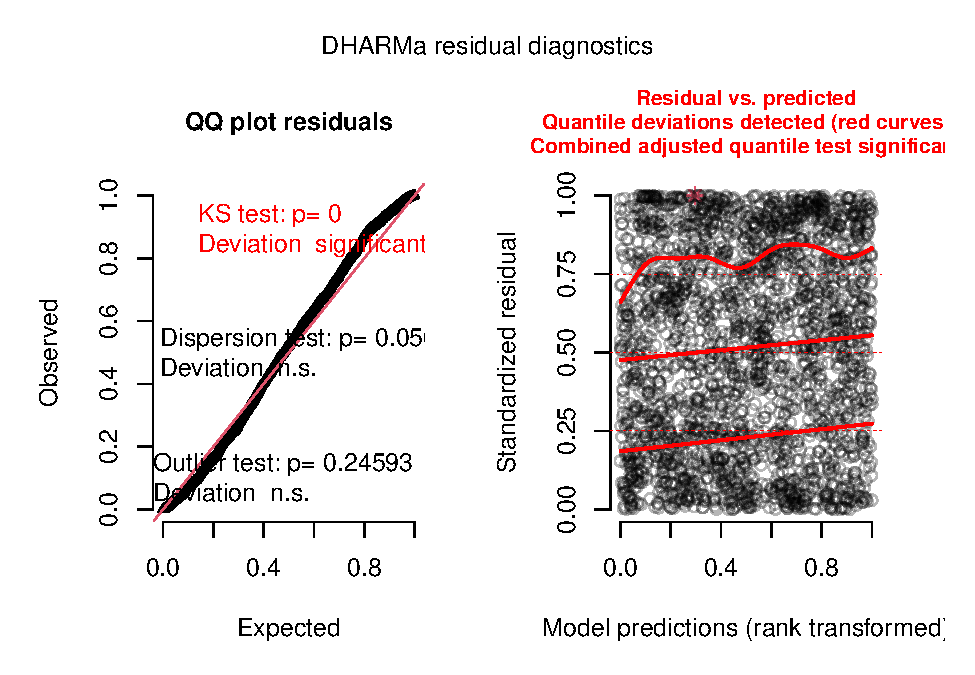
\includegraphics{lathyrus_ms3_3_after_rev_Ecology_files/figure-latex/unnamed-chunk-41-1.pdf}

\begin{verbatim}
## 
##  DHARMa zero-inflation test via comparison to expected zeros with
##  simulation under H0 = fitted model
## 
## data:  simulationOutput
## ratioObsSim = 1.3914, p-value < 2.2e-16
## alternative hypothesis: two.sided
\end{verbatim}

Zero inflation.

\hypertarget{try-with-betabinomial-1}{%
\subsubsection{Try with betabinomial}\label{try-with-betabinomial-1}}

\begin{Shaded}
\begin{Highlighting}[]
\NormalTok{mod\_seedpred\_bb\textless{}{-}}\KeywordTok{glmmTMB}\NormalTok{(}\KeywordTok{cbind}\NormalTok{(}\KeywordTok{round}\NormalTok{(n\_pred\_seeds),}\KeywordTok{round}\NormalTok{(n\_intact\_seeds))}\OperatorTok{\textasciitilde{}}
\StringTok{                     }\NormalTok{(}\KeywordTok{scale}\NormalTok{(mean\_}\DecValTok{3}\NormalTok{)}\OperatorTok{+}\KeywordTok{scale}\NormalTok{(mean\_}\DecValTok{4}\NormalTok{)}\OperatorTok{+}\KeywordTok{scale}\NormalTok{(mean\_}\DecValTok{5}\NormalTok{)}\OperatorTok{+}\KeywordTok{scale}\NormalTok{(mean\_}\DecValTok{6}\NormalTok{))}\OperatorTok{*}
\StringTok{                      }\NormalTok{FFD\_s\_y}\OperatorTok{+}\NormalTok{n\_fl\_s\_y}\OperatorTok{+}\NormalTok{(}\DecValTok{1}\OperatorTok{|}\NormalTok{id),}\DataTypeTok{data=}\KeywordTok{subset}\NormalTok{(data\_selag,n\_seeds}\OperatorTok{\textgreater{}}\DecValTok{0}\NormalTok{),}
                    \DataTypeTok{family=}\StringTok{"betabinomial"}\NormalTok{)}
\KeywordTok{summary}\NormalTok{(mod\_seedpred\_bb)}
\end{Highlighting}
\end{Shaded}

\begin{verbatim}
##  Family: betabinomial  ( logit )
## Formula:          
## cbind(round(n_pred_seeds), round(n_intact_seeds)) ~ (scale(mean_3) +  
##     scale(mean_4) + scale(mean_5) + scale(mean_6)) * FFD_s_y +  
##     n_fl_s_y + (1 | id)
## Data: subset(data_selag, n_seeds > 0)
## 
##      AIC      BIC   logLik deviance df.resid 
##   5339.2   5406.3  -2656.6   5313.2     1268 
## 
## Random effects:
## 
## Conditional model:
##  Groups Name        Variance Std.Dev.
##  id     (Intercept) 0.06597  0.2569  
## Number of obs: 1281, groups:  id, 593
## 
## Overdispersion parameter for betabinomial family (): 1.15 
## 
## Conditional model:
##                       Estimate Std. Error z value Pr(>|z|)    
## (Intercept)           -0.84346    0.05517 -15.289  < 2e-16 ***
## scale(mean_3)         -0.20163    0.07223  -2.792  0.00525 ** 
## scale(mean_4)          0.02973    0.06213   0.478  0.63233    
## scale(mean_5)          0.46942    0.07236   6.487 8.75e-11 ***
## scale(mean_6)          0.41522    0.06211   6.685 2.31e-11 ***
## FFD_s_y                0.03140    0.05865   0.535  0.59231    
## n_fl_s_y               0.17791    0.04409   4.035 5.46e-05 ***
## scale(mean_3):FFD_s_y  0.17398    0.08155   2.133  0.03289 *  
## scale(mean_4):FFD_s_y -0.15858    0.06662  -2.380  0.01729 *  
## scale(mean_5):FFD_s_y  0.02516    0.07756   0.324  0.74566    
## scale(mean_6):FFD_s_y -0.09364    0.06820  -1.373  0.16972    
## ---
## Signif. codes:  0 '***' 0.001 '**' 0.01 '*' 0.05 '.' 0.1 ' ' 1
\end{verbatim}

\hypertarget{model-diagnostics-5}{%
\subsubsection{Model diagnostics}\label{model-diagnostics-5}}

Simulate residuals of the model:

\begin{Shaded}
\begin{Highlighting}[]
\NormalTok{sim\_mod\_seedpred\_bb \textless{}{-}}\StringTok{ }\KeywordTok{simulateResiduals}\NormalTok{(}\DataTypeTok{fittedModel=}\NormalTok{mod\_seedpred\_bb,}\DataTypeTok{n=}\DecValTok{5000}\NormalTok{)}
\end{Highlighting}
\end{Shaded}

qq-plot and plot of residuals vs.~predicted:

\begin{Shaded}
\begin{Highlighting}[]
\KeywordTok{plot}\NormalTok{(sim\_mod\_seedpred\_bb,}\DataTypeTok{quantreg=}\NormalTok{T)}
\end{Highlighting}
\end{Shaded}

\includegraphics{lathyrus_ms3_3_after_rev_Ecology_files/figure-latex/unnamed-chunk-44-1.pdf}

\begin{Shaded}
\begin{Highlighting}[]
\KeywordTok{testDispersion}\NormalTok{(sim\_mod\_seedpred\_bb)}
\end{Highlighting}
\end{Shaded}

\includegraphics{lathyrus_ms3_3_after_rev_Ecology_files/figure-latex/unnamed-chunk-45-1.pdf}

\begin{verbatim}
## 
##  DHARMa nonparametric dispersion test via sd of residuals fitted vs.
##  simulated
## 
## data:  simulationOutput
## ratioObsSim = 0.85972, p-value = 0.0024
## alternative hypothesis: two.sided
\end{verbatim}

Slight underdispersion.

\begin{Shaded}
\begin{Highlighting}[]
\KeywordTok{testZeroInflation}\NormalTok{(sim\_mod\_seedpred\_bb)}
\end{Highlighting}
\end{Shaded}

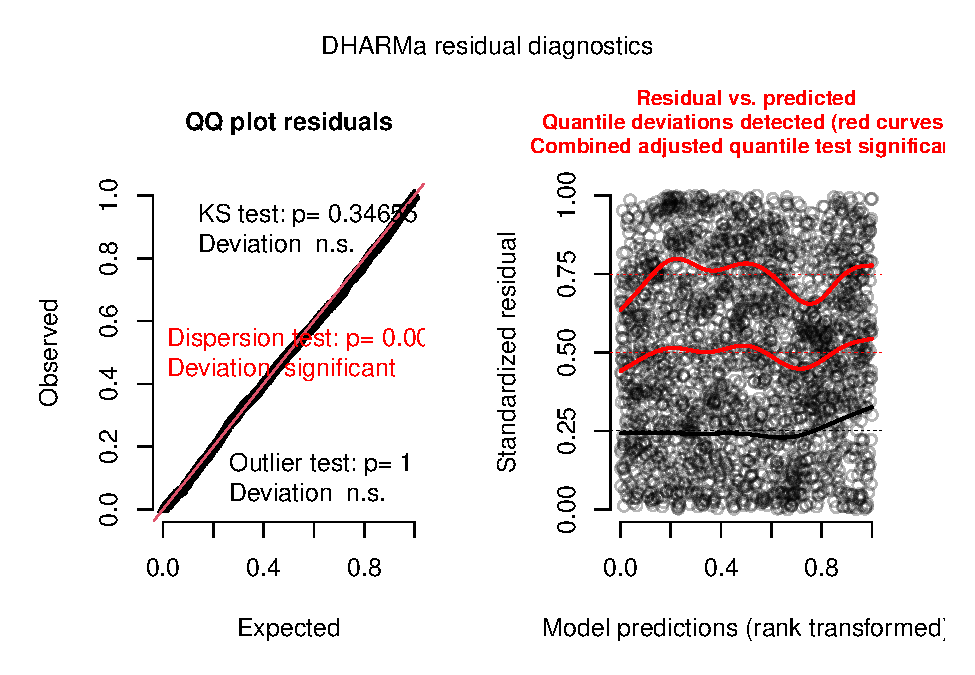
\includegraphics{lathyrus_ms3_3_after_rev_Ecology_files/figure-latex/unnamed-chunk-46-1.pdf}

\begin{verbatim}
## 
##  DHARMa zero-inflation test via comparison to expected zeros with
##  simulation under H0 = fitted model
## 
## data:  simulationOutput
## ratioObsSim = 1.0244, p-value = 0.4808
## alternative hypothesis: two.sided
\end{verbatim}

OK.

\begin{Shaded}
\begin{Highlighting}[]
\KeywordTok{anova}\NormalTok{(mod\_seedpred,mod\_seedpred\_bb)}
\end{Highlighting}
\end{Shaded}

\begin{verbatim}
## Data: subset(data_selag, n_seeds > 0)
## Models:
## mod_seedpred: cbind(round(n_pred_seeds), round(n_intact_seeds)) ~ (scale(mean_3) + , zi=~0, disp=~1
## mod_seedpred:     scale(mean_4) + scale(mean_5) + scale(mean_6)) * FFD_s_y + , zi=~0, disp=~1
## mod_seedpred:     n_fl_s_y + (1 | id), zi=~0, disp=~1
## mod_seedpred_bb: cbind(round(n_pred_seeds), round(n_intact_seeds)) ~ (scale(mean_3) + , zi=~0, disp=~1
## mod_seedpred_bb:     scale(mean_4) + scale(mean_5) + scale(mean_6)) * FFD_s_y + , zi=~0, disp=~1
## mod_seedpred_bb:     n_fl_s_y + (1 | id), zi=~0, disp=~1
##                 Df    AIC    BIC  logLik deviance  Chisq Chi Df Pr(>Chisq)    
## mod_seedpred    12 9018.9 9080.7 -4497.4   8994.9                             
## mod_seedpred_bb 13 5339.2 5406.3 -2656.6   5313.2 3681.6      1  < 2.2e-16 ***
## ---
## Signif. codes:  0 '***' 0.001 '**' 0.01 '*' 0.05 '.' 0.1 ' ' 1
\end{verbatim}

\begin{Shaded}
\begin{Highlighting}[]
\KeywordTok{AIC}\NormalTok{(mod\_seedpred,mod\_seedpred\_bb)}
\end{Highlighting}
\end{Shaded}

\begin{verbatim}
##                 df      AIC
## mod_seedpred    12 9018.873
## mod_seedpred_bb 13 5339.232
\end{verbatim}

Keep mod\_seedpred\_bb.

\hypertarget{table-1}{%
\subsection{Table 1}\label{table-1}}

\begin{Shaded}
\begin{Highlighting}[]
\KeywordTok{kable}\NormalTok{(}\KeywordTok{summary}\NormalTok{(mod\_grazing\_bb)}\OperatorTok{$}\NormalTok{coefficients,}\DataTypeTok{digits=}\KeywordTok{c}\NormalTok{(}\DecValTok{3}\NormalTok{,}\DecValTok{3}\NormalTok{,}\DecValTok{2}\NormalTok{,}\DecValTok{3}\NormalTok{))}
\end{Highlighting}
\end{Shaded}

\begin{table}

\centering
\begin{tabular}[t]{l|r|r|r|r}
\hline
  & Estimate & Std. Error & z value & Pr(>|z|)\\
\hline
(Intercept) & -2.232 & 0.090 & -24.66 & 0.000\\
\hline
scale(mean\_3) & 0.504 & 0.067 & 7.52 & 0.000\\
\hline
scale(mean\_4) & -0.333 & 0.064 & -5.19 & 0.000\\
\hline
scale(mean\_5) & -0.440 & 0.086 & -5.10 & 0.000\\
\hline
FFD\_s\_y & -0.256 & 0.073 & -3.50 & 0.000\\
\hline
n\_fl\_s\_y & 0.159 & 0.059 & 2.70 & 0.007\\
\hline
scale(mean\_3):FFD\_s\_y & 0.107 & 0.072 & 1.49 & 0.136\\
\hline
scale(mean\_4):FFD\_s\_y & -0.128 & 0.066 & -1.95 & 0.052\\
\hline
scale(mean\_5):FFD\_s\_y & 0.022 & 0.089 & 0.24 & 0.807\\
\hline
\end{tabular}
\centering
\begin{tabular}[t]{}
\hline

\hline
\end{tabular}
\centering
\begin{tabular}[t]{}
\hline

\hline
\end{tabular}
\end{table}

\begin{Shaded}
\begin{Highlighting}[]
\KeywordTok{kable}\NormalTok{(}\KeywordTok{summary}\NormalTok{(mod\_seedpred\_bb)}\OperatorTok{$}\NormalTok{coefficients,}\DataTypeTok{digits=}\KeywordTok{c}\NormalTok{(}\DecValTok{3}\NormalTok{,}\DecValTok{3}\NormalTok{,}\DecValTok{2}\NormalTok{,}\DecValTok{3}\NormalTok{))}
\end{Highlighting}
\end{Shaded}

\begin{table}

\centering
\begin{tabular}[t]{l|r|r|r|r}
\hline
  & Estimate & Std. Error & z value & Pr(>|z|)\\
\hline
(Intercept) & -0.843 & 0.055 & -15.29 & 0.000\\
\hline
scale(mean\_3) & -0.202 & 0.072 & -2.79 & 0.005\\
\hline
scale(mean\_4) & 0.030 & 0.062 & 0.48 & 0.632\\
\hline
scale(mean\_5) & 0.469 & 0.072 & 6.49 & 0.000\\
\hline
scale(mean\_6) & 0.415 & 0.062 & 6.69 & 0.000\\
\hline
FFD\_s\_y & 0.031 & 0.059 & 0.54 & 0.592\\
\hline
n\_fl\_s\_y & 0.178 & 0.044 & 4.03 & 0.000\\
\hline
scale(mean\_3):FFD\_s\_y & 0.174 & 0.082 & 2.13 & 0.033\\
\hline
scale(mean\_4):FFD\_s\_y & -0.159 & 0.067 & -2.38 & 0.017\\
\hline
scale(mean\_5):FFD\_s\_y & 0.025 & 0.078 & 0.32 & 0.746\\
\hline
scale(mean\_6):FFD\_s\_y & -0.094 & 0.068 & -1.37 & 0.170\\
\hline
\end{tabular}
\centering
\begin{tabular}[t]{}
\hline

\hline
\end{tabular}
\centering
\begin{tabular}[t]{}
\hline

\hline
\end{tabular}
\end{table}

\hypertarget{graphs-for-fig-2---part-1}{%
\subsection{Graphs for Fig 2 - Part 1}\label{graphs-for-fig-2---part-1}}

\begin{Shaded}
\begin{Highlighting}[]
\NormalTok{pred\_grazing\_mean3\textless{}{-}}\KeywordTok{ggpredict}\NormalTok{(mod\_grazing\_bb,}
                              \DataTypeTok{terms =} \KeywordTok{c}\NormalTok{(}\StringTok{"mean\_3 [all]"}\NormalTok{))}
\NormalTok{pred\_grazing\_mean4\textless{}{-}}\KeywordTok{ggpredict}\NormalTok{(mod\_grazing\_bb,}
                              \DataTypeTok{terms =} \KeywordTok{c}\NormalTok{(}\StringTok{"mean\_4 [all]"}\NormalTok{))}
\NormalTok{pred\_grazing\_mean5\textless{}{-}}\KeywordTok{ggpredict}\NormalTok{(mod\_grazing\_bb,}
                              \DataTypeTok{terms =} \KeywordTok{c}\NormalTok{(}\StringTok{"mean\_5 [all]"}\NormalTok{))}
\end{Highlighting}
\end{Shaded}

\begin{Shaded}
\begin{Highlighting}[]
\NormalTok{Fig\_}\DecValTok{2}\NormalTok{\_temps\_grazing\textless{}{-}}\KeywordTok{grid.arrange}\NormalTok{(}
  \KeywordTok{ggplot}\NormalTok{(data\_selag,}\KeywordTok{aes}\NormalTok{(}\DataTypeTok{x=}\NormalTok{mean\_}\DecValTok{3}\NormalTok{,}\DataTypeTok{y=}\NormalTok{grazing\_corr))}\OperatorTok{+}
\StringTok{    }\KeywordTok{geom\_point}\NormalTok{(}\DataTypeTok{size=}\DecValTok{3}\NormalTok{,}\DataTypeTok{alpha=}\FloatTok{0.05}\NormalTok{)}\OperatorTok{+}
\StringTok{    }\KeywordTok{geom\_ribbon}\NormalTok{(}\DataTypeTok{data=}\NormalTok{pred\_grazing\_mean3,}
                \KeywordTok{aes}\NormalTok{(x,predicted,}\DataTypeTok{ymin=}\NormalTok{conf.low,}\DataTypeTok{ymax=}\NormalTok{conf.high),}
                \DataTypeTok{fill=}\StringTok{"firebrick2"}\NormalTok{,}\DataTypeTok{alpha=}\FloatTok{0.3}\NormalTok{)}\OperatorTok{+}
\StringTok{    }\KeywordTok{geom\_line}\NormalTok{(}\DataTypeTok{data=}\NormalTok{pred\_grazing\_mean3,}\KeywordTok{aes}\NormalTok{(x,predicted),}
              \DataTypeTok{color=}\StringTok{"firebrick2"}\NormalTok{,}\DataTypeTok{size=}\DecValTok{1}\NormalTok{)}\OperatorTok{+}
\StringTok{    }\KeywordTok{my\_theme}\NormalTok{()}\OperatorTok{+}\KeywordTok{xlab}\NormalTok{(}\StringTok{"Mean March (ºC)"}\NormalTok{)}\OperatorTok{+}\KeywordTok{ylab}\NormalTok{(}\OtherTok{NULL}\NormalTok{)}\OperatorTok{+}
\StringTok{    }\KeywordTok{theme}\NormalTok{(}\DataTypeTok{plot.margin =} \KeywordTok{unit}\NormalTok{(}\KeywordTok{c}\NormalTok{(}\FloatTok{0.3}\NormalTok{,}\FloatTok{0.1}\NormalTok{,}\FloatTok{0.3}\NormalTok{,}\FloatTok{0.1}\NormalTok{), }\StringTok{"cm"}\NormalTok{))}\OperatorTok{+}
\StringTok{    }\KeywordTok{theme}\NormalTok{(}\DataTypeTok{axis.text.y=}\KeywordTok{element\_blank}\NormalTok{()),}
  \KeywordTok{ggplot}\NormalTok{(data\_selag,}\KeywordTok{aes}\NormalTok{(}\DataTypeTok{x=}\NormalTok{mean\_}\DecValTok{4}\NormalTok{,}\DataTypeTok{y=}\NormalTok{grazing\_corr))}\OperatorTok{+}
\StringTok{    }\KeywordTok{geom\_point}\NormalTok{(}\DataTypeTok{size=}\DecValTok{3}\NormalTok{,}\DataTypeTok{alpha=}\FloatTok{0.05}\NormalTok{)}\OperatorTok{+}
\StringTok{    }\KeywordTok{geom\_ribbon}\NormalTok{(}\DataTypeTok{data=}\NormalTok{pred\_grazing\_mean4,}
                \KeywordTok{aes}\NormalTok{(x,predicted,}\DataTypeTok{ymin=}\NormalTok{conf.low,}\DataTypeTok{ymax=}\NormalTok{conf.high),}
                \DataTypeTok{fill=}\StringTok{"firebrick2"}\NormalTok{,}\DataTypeTok{alpha=}\FloatTok{0.3}\NormalTok{)}\OperatorTok{+}
\StringTok{    }\KeywordTok{geom\_line}\NormalTok{(}\DataTypeTok{data=}\NormalTok{pred\_grazing\_mean4,}\KeywordTok{aes}\NormalTok{(x,predicted),}
              \DataTypeTok{color=}\StringTok{"firebrick2"}\NormalTok{,}\DataTypeTok{size=}\DecValTok{1}\NormalTok{)}\OperatorTok{+}
\StringTok{    }\KeywordTok{my\_theme}\NormalTok{()}\OperatorTok{+}\KeywordTok{xlab}\NormalTok{(}\StringTok{"Mean April (ºC)"}\NormalTok{)}\OperatorTok{+}\KeywordTok{ylab}\NormalTok{(}\OtherTok{NULL}\NormalTok{)}\OperatorTok{+}
\StringTok{    }\KeywordTok{theme}\NormalTok{(}\DataTypeTok{plot.margin =} \KeywordTok{unit}\NormalTok{(}\KeywordTok{c}\NormalTok{(}\FloatTok{0.3}\NormalTok{,}\FloatTok{0.1}\NormalTok{,}\FloatTok{0.3}\NormalTok{,}\FloatTok{0.1}\NormalTok{), }\StringTok{"cm"}\NormalTok{))}\OperatorTok{+}
\StringTok{    }\KeywordTok{theme}\NormalTok{(}\DataTypeTok{axis.text.y=}\KeywordTok{element\_blank}\NormalTok{()),}
  \KeywordTok{ggplot}\NormalTok{(data\_selag,}\KeywordTok{aes}\NormalTok{(}\DataTypeTok{x=}\NormalTok{mean\_}\DecValTok{5}\NormalTok{,}\DataTypeTok{y=}\NormalTok{grazing\_corr))}\OperatorTok{+}
\StringTok{    }\KeywordTok{geom\_point}\NormalTok{(}\DataTypeTok{size=}\DecValTok{3}\NormalTok{,}\DataTypeTok{alpha=}\FloatTok{0.05}\NormalTok{)}\OperatorTok{+}
\StringTok{    }\KeywordTok{geom\_ribbon}\NormalTok{(}\DataTypeTok{data=}\NormalTok{pred\_grazing\_mean5,}
                \KeywordTok{aes}\NormalTok{(x,predicted,}\DataTypeTok{ymin=}\NormalTok{conf.low,}\DataTypeTok{ymax=}\NormalTok{conf.high),}
                \DataTypeTok{fill=}\StringTok{"firebrick2"}\NormalTok{,}\DataTypeTok{alpha=}\FloatTok{0.3}\NormalTok{)}\OperatorTok{+}
\StringTok{    }\KeywordTok{geom\_line}\NormalTok{(}\DataTypeTok{data=}\NormalTok{pred\_grazing\_mean5,}\KeywordTok{aes}\NormalTok{(x,predicted),}
              \DataTypeTok{color=}\StringTok{"firebrick2"}\NormalTok{,}\DataTypeTok{size=}\DecValTok{1}\NormalTok{)}\OperatorTok{+}
\StringTok{    }\KeywordTok{my\_theme}\NormalTok{()}\OperatorTok{+}\KeywordTok{xlab}\NormalTok{(}\StringTok{"Mean May (ºC)"}\NormalTok{)}\OperatorTok{+}\KeywordTok{ylab}\NormalTok{(}\OtherTok{NULL}\NormalTok{)}\OperatorTok{+}
\StringTok{    }\KeywordTok{theme}\NormalTok{(}\DataTypeTok{plot.margin =} \KeywordTok{unit}\NormalTok{(}\KeywordTok{c}\NormalTok{(}\FloatTok{0.3}\NormalTok{,}\FloatTok{0.1}\NormalTok{,}\FloatTok{0.3}\NormalTok{,}\FloatTok{0.1}\NormalTok{), }\StringTok{"cm"}\NormalTok{))}\OperatorTok{+}
\StringTok{    }\KeywordTok{theme}\NormalTok{(}\DataTypeTok{axis.text.y=}\KeywordTok{element\_blank}\NormalTok{()),}
  \DataTypeTok{ncol=}\DecValTok{3}\NormalTok{)}
\end{Highlighting}
\end{Shaded}

\includegraphics{lathyrus_ms3_3_after_rev_Ecology_files/figure-latex/unnamed-chunk-50-1.pdf}

\begin{Shaded}
\begin{Highlighting}[]
\KeywordTok{ggsave}\NormalTok{(}\DataTypeTok{filename=}\StringTok{"output/figures/Fig\_2\_temps\_grazing.tiff"}\NormalTok{,}
       \DataTypeTok{plot=}\NormalTok{Fig\_}\DecValTok{2}\NormalTok{\_temps\_grazing,}\DataTypeTok{device=}\StringTok{"tiff"}\NormalTok{,}\DataTypeTok{width=}\DecValTok{15}\NormalTok{,}\DataTypeTok{height=}\DecValTok{8}\NormalTok{,}\DataTypeTok{units=}\StringTok{"cm"}\NormalTok{,}
       \DataTypeTok{dpi=}\DecValTok{300}\NormalTok{,}\DataTypeTok{compression=}\StringTok{"lzw"}\NormalTok{)}
\end{Highlighting}
\end{Shaded}

\begin{Shaded}
\begin{Highlighting}[]
\NormalTok{pred\_seedpred\_mean3\_FFD\textless{}{-}}\KeywordTok{ggpredict}\NormalTok{(mod\_seedpred\_bb,}
                        \DataTypeTok{terms =} \KeywordTok{c}\NormalTok{(}\StringTok{"mean\_3 [all]"}\NormalTok{,}\StringTok{"FFD\_s\_y [{-}2.6:3.9 by=.5]"}\NormalTok{))}
\NormalTok{pred\_seedpred\_mean4\_FFD\textless{}{-}}\KeywordTok{ggpredict}\NormalTok{(mod\_seedpred\_bb,}
                        \DataTypeTok{terms =} \KeywordTok{c}\NormalTok{(}\StringTok{"mean\_4 [all]"}\NormalTok{,}\StringTok{"FFD\_s\_y [{-}2.6:3.9 by=.5]"}\NormalTok{))}
\NormalTok{pred\_seedpred\_mean5\textless{}{-}}\KeywordTok{ggpredict}\NormalTok{(mod\_seedpred\_bb,}
                              \DataTypeTok{terms =} \KeywordTok{c}\NormalTok{(}\StringTok{"mean\_5 [all]"}\NormalTok{))}
\NormalTok{pred\_seedpred\_mean6\textless{}{-}}\KeywordTok{ggpredict}\NormalTok{(mod\_seedpred\_bb,}
                              \DataTypeTok{terms =} \KeywordTok{c}\NormalTok{(}\StringTok{"mean\_6 [all]"}\NormalTok{))}
\end{Highlighting}
\end{Shaded}

\begin{Shaded}
\begin{Highlighting}[]
\NormalTok{Fig\_}\DecValTok{2}\NormalTok{\_temps\_seedpred\textless{}{-}}\KeywordTok{grid.arrange}\NormalTok{(}
  \KeywordTok{ggplot}\NormalTok{(pred\_seedpred\_mean3\_FFD,}\KeywordTok{aes}\NormalTok{(x,predicted,}\DataTypeTok{colour=}\NormalTok{group,}\DataTypeTok{fill=}\NormalTok{group))}\OperatorTok{+}
\StringTok{    }\KeywordTok{geom\_line}\NormalTok{(}\KeywordTok{aes}\NormalTok{(}\DataTypeTok{color=}\KeywordTok{as.numeric}\NormalTok{(}\KeywordTok{as.character}\NormalTok{(group))),}\DataTypeTok{size=}\FloatTok{0.6}\NormalTok{)}\OperatorTok{+}\KeywordTok{my\_theme}\NormalTok{()}\OperatorTok{+}
\StringTok{    }\KeywordTok{scale\_color\_viridis}\NormalTok{()}\OperatorTok{+}
\StringTok{    }\KeywordTok{theme}\NormalTok{(}\DataTypeTok{axis.text.y=}\KeywordTok{element\_blank}\NormalTok{())}\OperatorTok{+}
\StringTok{    }\KeywordTok{scale\_y\_continuous}\NormalTok{(}\DataTypeTok{breaks =} \KeywordTok{seq}\NormalTok{(}\DecValTok{0}\NormalTok{, }\DecValTok{1}\NormalTok{, }\DataTypeTok{by =} \FloatTok{0.25}\NormalTok{))}\OperatorTok{+}\KeywordTok{ylim}\NormalTok{(}\DecValTok{0}\NormalTok{,}\DecValTok{1}\NormalTok{)}\OperatorTok{+}
\StringTok{    }\KeywordTok{theme}\NormalTok{(}\DataTypeTok{legend.justification=}\KeywordTok{c}\NormalTok{(}\FloatTok{1.1}\NormalTok{,}\FloatTok{0.99}\NormalTok{),}\DataTypeTok{legend.position=}\KeywordTok{c}\NormalTok{(}\FloatTok{1.07}\NormalTok{,}\FloatTok{0.89}\NormalTok{),}
        \DataTypeTok{legend.direction=}\StringTok{"horizontal"}\NormalTok{,}\DataTypeTok{legend.title=}\KeywordTok{element\_blank}\NormalTok{())}\OperatorTok{+}
\StringTok{    }\KeywordTok{annotate}\NormalTok{(}\StringTok{"text"}\NormalTok{,}\DataTypeTok{x=}\FloatTok{0.8}\NormalTok{,}\DataTypeTok{y=}\FloatTok{0.98}\NormalTok{,}\DataTypeTok{label=}\StringTok{"FFD: early          late"}\NormalTok{,}
             \DataTypeTok{family=}\StringTok{"serif"}\NormalTok{,}\DataTypeTok{size=}\DecValTok{5}\NormalTok{)}\OperatorTok{+}
\StringTok{    }\KeywordTok{xlab}\NormalTok{(}\StringTok{"Mean March (ºC)"}\NormalTok{)}\OperatorTok{+}\KeywordTok{ylab}\NormalTok{(}\OtherTok{NULL}\NormalTok{)}\OperatorTok{+}
\StringTok{    }\KeywordTok{theme}\NormalTok{(}\DataTypeTok{plot.margin =} \KeywordTok{unit}\NormalTok{(}\KeywordTok{c}\NormalTok{(}\FloatTok{0.3}\NormalTok{,}\FloatTok{0.1}\NormalTok{,}\FloatTok{0.3}\NormalTok{,}\FloatTok{0.1}\NormalTok{), }\StringTok{"cm"}\NormalTok{)),}
  \KeywordTok{ggplot}\NormalTok{(pred\_seedpred\_mean4\_FFD,}\KeywordTok{aes}\NormalTok{(x,predicted,}\DataTypeTok{colour=}\NormalTok{group,}\DataTypeTok{fill=}\NormalTok{group))}\OperatorTok{+}
\StringTok{    }\KeywordTok{geom\_line}\NormalTok{(}\KeywordTok{aes}\NormalTok{(}\DataTypeTok{color=}\KeywordTok{as.numeric}\NormalTok{(}\KeywordTok{as.character}\NormalTok{(group))),}\DataTypeTok{size=}\FloatTok{0.6}\NormalTok{)}\OperatorTok{+}\KeywordTok{my\_theme}\NormalTok{()}\OperatorTok{+}
\StringTok{    }\KeywordTok{scale\_color\_viridis}\NormalTok{()}\OperatorTok{+}
\StringTok{    }\KeywordTok{theme}\NormalTok{(}\DataTypeTok{axis.text.y=}\KeywordTok{element\_blank}\NormalTok{())}\OperatorTok{+}
\StringTok{    }\KeywordTok{scale\_y\_continuous}\NormalTok{(}\DataTypeTok{breaks =} \KeywordTok{seq}\NormalTok{(}\DecValTok{0}\NormalTok{, }\DecValTok{1}\NormalTok{, }\DataTypeTok{by =} \FloatTok{0.25}\NormalTok{))}\OperatorTok{+}\KeywordTok{ylim}\NormalTok{(}\DecValTok{0}\NormalTok{,}\DecValTok{1}\NormalTok{)}\OperatorTok{+}
\StringTok{    }\KeywordTok{xlab}\NormalTok{(}\StringTok{"Mean April (ºC)"}\NormalTok{)}\OperatorTok{+}\KeywordTok{ylab}\NormalTok{(}\OtherTok{NULL}\NormalTok{)}\OperatorTok{+}
\StringTok{    }\KeywordTok{theme}\NormalTok{(}\DataTypeTok{plot.margin =} \KeywordTok{unit}\NormalTok{(}\KeywordTok{c}\NormalTok{(}\FloatTok{0.3}\NormalTok{,}\FloatTok{0.1}\NormalTok{,}\FloatTok{0.3}\NormalTok{,}\FloatTok{0.1}\NormalTok{), }\StringTok{"cm"}\NormalTok{)),}
  \KeywordTok{ggplot}\NormalTok{(data\_selag,}\KeywordTok{aes}\NormalTok{(}\DataTypeTok{x=}\NormalTok{mean\_}\DecValTok{5}\NormalTok{,}\DataTypeTok{y=}\NormalTok{prop\_pred\_seeds))}\OperatorTok{+}
\StringTok{    }\KeywordTok{geom\_point}\NormalTok{(}\DataTypeTok{size=}\DecValTok{3}\NormalTok{,}\DataTypeTok{alpha=}\FloatTok{0.05}\NormalTok{)}\OperatorTok{+}
\StringTok{    }\KeywordTok{geom\_ribbon}\NormalTok{(}\DataTypeTok{data=}\NormalTok{pred\_seedpred\_mean5,}
                \KeywordTok{aes}\NormalTok{(x,predicted,}\DataTypeTok{ymin=}\NormalTok{conf.low,}\DataTypeTok{ymax=}\NormalTok{conf.high),}
                \DataTypeTok{fill=}\StringTok{"firebrick2"}\NormalTok{,}\DataTypeTok{alpha=}\FloatTok{0.3}\NormalTok{)}\OperatorTok{+}
\StringTok{    }\KeywordTok{geom\_line}\NormalTok{(}\DataTypeTok{data=}\NormalTok{pred\_seedpred\_mean5,}\KeywordTok{aes}\NormalTok{(x,predicted),}
              \DataTypeTok{color=}\StringTok{"firebrick2"}\NormalTok{,}\DataTypeTok{size=}\DecValTok{1}\NormalTok{)}\OperatorTok{+}
\StringTok{    }\KeywordTok{my\_theme}\NormalTok{()}\OperatorTok{+}\KeywordTok{xlab}\NormalTok{(}\StringTok{"Mean May (ºC)"}\NormalTok{)}\OperatorTok{+}\KeywordTok{ylab}\NormalTok{(}\OtherTok{NULL}\NormalTok{)}\OperatorTok{+}
\StringTok{    }\KeywordTok{theme}\NormalTok{(}\DataTypeTok{plot.margin =} \KeywordTok{unit}\NormalTok{(}\KeywordTok{c}\NormalTok{(}\FloatTok{0.3}\NormalTok{,}\FloatTok{0.1}\NormalTok{,}\FloatTok{0.3}\NormalTok{,}\FloatTok{0.1}\NormalTok{), }\StringTok{"cm"}\NormalTok{))}\OperatorTok{+}
\StringTok{    }\KeywordTok{theme}\NormalTok{(}\DataTypeTok{axis.text.y=}\KeywordTok{element\_blank}\NormalTok{()),}
  \KeywordTok{ggplot}\NormalTok{(data\_selag,}\KeywordTok{aes}\NormalTok{(}\DataTypeTok{x=}\NormalTok{mean\_}\DecValTok{6}\NormalTok{,}\DataTypeTok{y=}\NormalTok{prop\_pred\_seeds))}\OperatorTok{+}
\StringTok{    }\KeywordTok{geom\_point}\NormalTok{(}\DataTypeTok{size=}\DecValTok{3}\NormalTok{,}\DataTypeTok{alpha=}\FloatTok{0.05}\NormalTok{)}\OperatorTok{+}
\StringTok{    }\KeywordTok{geom\_ribbon}\NormalTok{(}\DataTypeTok{data=}\NormalTok{pred\_seedpred\_mean6,}
                \KeywordTok{aes}\NormalTok{(x,predicted,}\DataTypeTok{ymin=}\NormalTok{conf.low,}\DataTypeTok{ymax=}\NormalTok{conf.high),}
                \DataTypeTok{fill=}\StringTok{"firebrick2"}\NormalTok{,}\DataTypeTok{alpha=}\FloatTok{0.3}\NormalTok{)}\OperatorTok{+}
\StringTok{    }\KeywordTok{geom\_line}\NormalTok{(}\DataTypeTok{data=}\NormalTok{pred\_seedpred\_mean6,}\KeywordTok{aes}\NormalTok{(x,predicted),}
              \DataTypeTok{color=}\StringTok{"firebrick2"}\NormalTok{,}\DataTypeTok{size=}\DecValTok{1}\NormalTok{)}\OperatorTok{+}
\StringTok{    }\KeywordTok{my\_theme}\NormalTok{()}\OperatorTok{+}\KeywordTok{xlab}\NormalTok{(}\StringTok{"Mean June (ºC)"}\NormalTok{)}\OperatorTok{+}\KeywordTok{ylab}\NormalTok{(}\OtherTok{NULL}\NormalTok{)}\OperatorTok{+}
\StringTok{    }\KeywordTok{theme}\NormalTok{(}\DataTypeTok{plot.margin =} \KeywordTok{unit}\NormalTok{(}\KeywordTok{c}\NormalTok{(}\FloatTok{0.3}\NormalTok{,}\FloatTok{0.1}\NormalTok{,}\FloatTok{0.3}\NormalTok{,}\FloatTok{0.1}\NormalTok{), }\StringTok{"cm"}\NormalTok{))}\OperatorTok{+}
\StringTok{    }\KeywordTok{theme}\NormalTok{(}\DataTypeTok{axis.text.y=}\KeywordTok{element\_blank}\NormalTok{()),}
  \DataTypeTok{ncol=}\DecValTok{4}\NormalTok{)}
\end{Highlighting}
\end{Shaded}

\includegraphics{lathyrus_ms3_3_after_rev_Ecology_files/figure-latex/unnamed-chunk-52-1.pdf}

\begin{Shaded}
\begin{Highlighting}[]
\KeywordTok{ggsave}\NormalTok{(}\DataTypeTok{filename=}\StringTok{"output/figures/Fig\_2\_temps\_seedpred.tiff"}\NormalTok{,}
       \DataTypeTok{plot=}\NormalTok{Fig\_}\DecValTok{2}\NormalTok{\_temps\_seedpred,}\DataTypeTok{device=}\StringTok{"tiff"}\NormalTok{,}\DataTypeTok{width=}\DecValTok{20}\NormalTok{,}\DataTypeTok{height=}\DecValTok{8}\NormalTok{,}\DataTypeTok{units=}\StringTok{"cm"}\NormalTok{,}
       \DataTypeTok{dpi=}\DecValTok{300}\NormalTok{,}\DataTypeTok{compression=}\StringTok{"lzw"}\NormalTok{)}
\end{Highlighting}
\end{Shaded}

\hypertarget{h3---part-2}{%
\section{H3 - Part 2}\label{h3---part-2}}

Differences in the intensity of biotic interactions among years, and in
the covariance between FFD and biotic interaction intensities, cause
differences in selection on flowering time.

In this phenotypic selection model, we use: fitness relativized within
years, FFD and n\_fl standardized within years,interactions and
covariances standardized accross years. Main effects of interactions and
covariances are not included because fitness was relativized within
years.

N = 2376

\begin{Shaded}
\begin{Highlighting}[]
\CommentTok{\# Add yearly mean values of biotic interaction to dataset }
\NormalTok{data\_selag\_means\textless{}{-}data\_selag}\OperatorTok{\%\textgreater{}\%}
\StringTok{  }\KeywordTok{group\_by}\NormalTok{(year)}\OperatorTok{\%\textgreater{}\%}
\StringTok{  }\NormalTok{dplyr}\OperatorTok{::}\KeywordTok{summarise}\NormalTok{(}\DataTypeTok{grazing\_mean=}\KeywordTok{mean}\NormalTok{(grazing\_corr,}\DataTypeTok{na.rm=}\NormalTok{T),}
                   \DataTypeTok{prop\_pred\_seeds\_mean=}\KeywordTok{mean}\NormalTok{(prop\_pred\_seeds,}\DataTypeTok{na.rm=}\NormalTok{T))}
\NormalTok{data\_selag\textless{}{-}data\_selag}\OperatorTok{\%\textgreater{}\%}\KeywordTok{left\_join}\NormalTok{(data\_selag\_means,}\DataTypeTok{by=}\StringTok{"year"}\NormalTok{)}
\end{Highlighting}
\end{Shaded}

\begin{Shaded}
\begin{Highlighting}[]
\CommentTok{\# Calculate covariance interactions {-} fitness for each  year}
\NormalTok{covar\_graz\_FFD\textless{}{-}data\_selag}\OperatorTok{\%\textgreater{}\%}
\StringTok{  }\KeywordTok{group\_by}\NormalTok{(year)}\OperatorTok{\%\textgreater{}\%}
\StringTok{  }\KeywordTok{do}\NormalTok{(}\DataTypeTok{graz\_FFD =} \KeywordTok{tidy}\NormalTok{(}\KeywordTok{glm}\NormalTok{(}\KeywordTok{cbind}\NormalTok{(grazing\_success,grazing\_failure)}\OperatorTok{\textasciitilde{}}\NormalTok{FFD\_s\_y, }
                             \DataTypeTok{data =}\NormalTok{ .,}\DataTypeTok{family=}\StringTok{"binomial"}\NormalTok{))) }\OperatorTok{\%\textgreater{}\%}\StringTok{ }
\StringTok{  }\KeywordTok{unnest}\NormalTok{(graz\_FFD)}\OperatorTok{\%\textgreater{}\%}
\StringTok{  }\KeywordTok{filter}\NormalTok{(term}\OperatorTok{==}\StringTok{"FFD\_s\_y"}\NormalTok{)}\OperatorTok{\%\textgreater{}\%}
\StringTok{  }\KeywordTok{select}\NormalTok{(year,estimate)}\OperatorTok{\%\textgreater{}\%}
\StringTok{  }\KeywordTok{rename}\NormalTok{(}\DataTypeTok{covar\_graz\_FFD=}\NormalTok{estimate)}

\NormalTok{covar\_seedpred\_FFD\textless{}{-}data\_selag}\OperatorTok{\%\textgreater{}\%}
\StringTok{  }\KeywordTok{filter}\NormalTok{(n\_seeds}\OperatorTok{\textgreater{}}\DecValTok{0}\NormalTok{)}\OperatorTok{\%\textgreater{}\%}
\StringTok{  }\KeywordTok{filter}\NormalTok{(}\OperatorTok{!}\KeywordTok{is.na}\NormalTok{(n\_intact\_seeds))}\OperatorTok{\%\textgreater{}\%}
\StringTok{  }\KeywordTok{group\_by}\NormalTok{(year)}\OperatorTok{\%\textgreater{}\%}
\StringTok{  }\KeywordTok{do}\NormalTok{(}\DataTypeTok{seedpred\_FFD =} \KeywordTok{tidy}\NormalTok{(}\KeywordTok{glm}\NormalTok{(}\KeywordTok{cbind}\NormalTok{(}\KeywordTok{round}\NormalTok{(n\_pred\_seeds),}\KeywordTok{round}\NormalTok{(n\_intact\_seeds))}\OperatorTok{\textasciitilde{}}
\StringTok{                               }\NormalTok{FFD\_s\_y,}\DataTypeTok{data =}\NormalTok{ .,}
                             \DataTypeTok{family=}\StringTok{"binomial"}\NormalTok{))) }\OperatorTok{\%\textgreater{}\%}\StringTok{ }
\StringTok{  }\KeywordTok{unnest}\NormalTok{(seedpred\_FFD)}\OperatorTok{\%\textgreater{}\%}
\StringTok{  }\KeywordTok{filter}\NormalTok{(term}\OperatorTok{==}\StringTok{"FFD\_s\_y"}\NormalTok{)}\OperatorTok{\%\textgreater{}\%}
\StringTok{  }\KeywordTok{select}\NormalTok{(year,estimate)}\OperatorTok{\%\textgreater{}\%}
\StringTok{  }\KeywordTok{rename}\NormalTok{(}\DataTypeTok{covar\_seedpred\_FFD=}\NormalTok{estimate)}

\NormalTok{data\_selag\_means\textless{}{-}data\_selag\_means}\OperatorTok{\%\textgreater{}\%}
\StringTok{  }\KeywordTok{full\_join}\NormalTok{(covar\_graz\_FFD)}\OperatorTok{\%\textgreater{}\%}
\StringTok{  }\KeywordTok{full\_join}\NormalTok{(covar\_seedpred\_FFD)}

\CommentTok{\# Add yearly covariances interactions {-} fitness to dataset }
\NormalTok{data\_selag\textless{}{-}data\_selag}\OperatorTok{\%\textgreater{}\%}\KeywordTok{left\_join}\NormalTok{(data\_selag\_means[}\KeywordTok{c}\NormalTok{(}\DecValTok{1}\NormalTok{,}\DecValTok{4}\OperatorTok{:}\DecValTok{5}\NormalTok{)],}\DataTypeTok{by=}\StringTok{"year"}\NormalTok{)}
\end{Highlighting}
\end{Shaded}

\begin{Shaded}
\begin{Highlighting}[]
\NormalTok{mod\_int\_sel\_GLMM\textless{}{-}}\KeywordTok{glmmTMB}\NormalTok{(fitness\_rel\_y }\OperatorTok{\textasciitilde{}}\StringTok{ }\NormalTok{FFD\_s\_y}\OperatorTok{+}\NormalTok{n\_fl\_s\_y}\OperatorTok{+}
\StringTok{                            }\NormalTok{FFD\_s\_y}\OperatorTok{:}\KeywordTok{scale}\NormalTok{(grazing\_mean)}\OperatorTok{+}
\StringTok{                            }\NormalTok{FFD\_s\_y}\OperatorTok{:}\KeywordTok{scale}\NormalTok{(covar\_graz\_FFD)}\OperatorTok{+}
\StringTok{                            }\NormalTok{FFD\_s\_y}\OperatorTok{:}\KeywordTok{scale}\NormalTok{(prop\_pred\_seeds\_mean)}\OperatorTok{+}
\StringTok{                            }\NormalTok{FFD\_s\_y}\OperatorTok{:}\KeywordTok{scale}\NormalTok{(covar\_seedpred\_FFD)}\OperatorTok{+}
\StringTok{                            }\NormalTok{(}\DecValTok{1}\OperatorTok{|}\NormalTok{id),data\_selag,}\DataTypeTok{family=}\StringTok{"gaussian"}\NormalTok{)}
\NormalTok{mod\_int\_sel\_GLMM\_lmer\textless{}{-}}\KeywordTok{lmer}\NormalTok{(fitness\_rel\_y }\OperatorTok{\textasciitilde{}}\StringTok{ }\NormalTok{FFD\_s\_y}\OperatorTok{+}\NormalTok{n\_fl\_s\_y}\OperatorTok{+}
\StringTok{                              }\NormalTok{FFD\_s\_y}\OperatorTok{:}\KeywordTok{scale}\NormalTok{(grazing\_mean)}\OperatorTok{+}
\StringTok{                              }\NormalTok{FFD\_s\_y}\OperatorTok{:}\KeywordTok{scale}\NormalTok{(covar\_graz\_FFD)}\OperatorTok{+}
\StringTok{                              }\NormalTok{FFD\_s\_y}\OperatorTok{:}\KeywordTok{scale}\NormalTok{(prop\_pred\_seeds\_mean)}\OperatorTok{+}
\StringTok{                              }\NormalTok{FFD\_s\_y}\OperatorTok{:}\KeywordTok{scale}\NormalTok{(covar\_seedpred\_FFD)}\OperatorTok{+}
\StringTok{                              }\NormalTok{(}\DecValTok{1}\OperatorTok{|}\NormalTok{id),data\_selag)}
\NormalTok{mod\_int\_sel\_LM\textless{}{-}}\KeywordTok{lm}\NormalTok{(fitness\_rel\_y }\OperatorTok{\textasciitilde{}}\StringTok{ }\NormalTok{FFD\_s\_y}\OperatorTok{+}\NormalTok{n\_fl\_s\_y}\OperatorTok{+}
\StringTok{                         }\NormalTok{FFD\_s\_y}\OperatorTok{:}\KeywordTok{scale}\NormalTok{(grazing\_mean)}\OperatorTok{+}
\StringTok{                            }\NormalTok{FFD\_s\_y}\OperatorTok{:}\KeywordTok{scale}\NormalTok{(covar\_graz\_FFD)}\OperatorTok{+}
\StringTok{                            }\NormalTok{FFD\_s\_y}\OperatorTok{:}\KeywordTok{scale}\NormalTok{(prop\_pred\_seeds\_mean)}\OperatorTok{+}
\StringTok{                            }\NormalTok{FFD\_s\_y}\OperatorTok{:}\KeywordTok{scale}\NormalTok{(covar\_seedpred\_FFD),}
                   \KeywordTok{subset}\NormalTok{(data\_selag,}\OperatorTok{!}\KeywordTok{is.na}\NormalTok{(fitness\_rel\_y)}\OperatorTok{\&}
\StringTok{                            }\OperatorTok{!}\KeywordTok{is.na}\NormalTok{(FFD\_s\_y)}\OperatorTok{\&!}\KeywordTok{is.na}\NormalTok{(n\_fl\_s\_y)}\OperatorTok{\&}
\StringTok{                            }\OperatorTok{!}\KeywordTok{is.na}\NormalTok{(grazing\_mean)}\OperatorTok{\&}
\StringTok{                            }\OperatorTok{!}\KeywordTok{is.na}\NormalTok{(prop\_pred\_seeds\_mean)))}
\CommentTok{\# Results of models (t{-}tests)}
\KeywordTok{kable}\NormalTok{(}\KeywordTok{summary}\NormalTok{(mod\_int\_sel\_GLMM)}\OperatorTok{$}\NormalTok{coefficients,}\DataTypeTok{digits=}\KeywordTok{c}\NormalTok{(}\DecValTok{3}\NormalTok{,}\DecValTok{3}\NormalTok{,}\DecValTok{0}\NormalTok{,}\DecValTok{2}\NormalTok{,}\DecValTok{3}\NormalTok{))}
\end{Highlighting}
\end{Shaded}

\begin{table}

\centering
\begin{tabular}[t]{l|r|r|r|r}
\hline
  & Estimate & Std. Error & z value & Pr(>|z|)\\
\hline
(Intercept) & 1.025 & 0.045 & 23 & 0.00\\
\hline
FFD\_s\_y & -0.299 & 0.052 & -6 & 0.00\\
\hline
n\_fl\_s\_y & 0.389 & 0.049 & 8 & 0.00\\
\hline
FFD\_s\_y:scale(grazing\_mean) & 0.108 & 0.039 & 3 & 0.01\\
\hline
FFD\_s\_y:scale(covar\_graz\_FFD) & -0.027 & 0.049 & -1 & 0.58\\
\hline
FFD\_s\_y:scale(prop\_pred\_seeds\_mean) & 0.003 & 0.039 & 0 & 0.93\\
\hline
FFD\_s\_y:scale(covar\_seedpred\_FFD) & -0.033 & 0.035 & -1 & 0.34\\
\hline
\end{tabular}
\centering
\begin{tabular}[t]{}
\hline

\hline
\end{tabular}
\centering
\begin{tabular}[t]{}
\hline

\hline
\end{tabular}
\end{table}

\begin{Shaded}
\begin{Highlighting}[]
\CommentTok{\# Analysis of deviance (Wald chi‐square tests for GLMM)}
\KeywordTok{kable}\NormalTok{(}\KeywordTok{Anova}\NormalTok{(mod\_int\_sel\_GLMM),}\DataTypeTok{digits=}\KeywordTok{c}\NormalTok{(}\DecValTok{2}\NormalTok{,}\DecValTok{1}\NormalTok{,}\DecValTok{3}\NormalTok{))}
\end{Highlighting}
\end{Shaded}

\begin{longtable}[]{@{}lrrr@{}}
\toprule
& Chisq & Df & Pr(\textgreater Chisq)\tabularnewline
\midrule
\endhead
FFD\_s\_y & 32.42 & 1 & 0.000\tabularnewline
n\_fl\_s\_y & 63.28 & 1 & 0.000\tabularnewline
FFD\_s\_y:scale(grazing\_mean) & 7.83 & 1 & 0.005\tabularnewline
FFD\_s\_y:scale(covar\_graz\_FFD) & 0.30 & 1 & 0.581\tabularnewline
FFD\_s\_y:scale(prop\_pred\_seeds\_mean) & 0.01 & 1 &
0.930\tabularnewline
FFD\_s\_y:scale(covar\_seedpred\_FFD) & 0.91 & 1 & 0.341\tabularnewline
\bottomrule
\end{longtable}

Significant effect of yearly mean grazing on selection (but we have seen
that the significance is driven by the year 2017).

\hypertarget{model-diagnostics-6}{%
\subsection{Model diagnostics}\label{model-diagnostics-6}}

Simulate residuals of the model:

\begin{Shaded}
\begin{Highlighting}[]
\NormalTok{simulationOutput\_mod\_int\_sel\_GLMM \textless{}{-}}\StringTok{ }
\StringTok{  }\KeywordTok{simulateResiduals}\NormalTok{(}\DataTypeTok{fittedModel =}\NormalTok{ mod\_int\_sel\_GLMM, }\DataTypeTok{n =} \DecValTok{5000}\NormalTok{)}
\end{Highlighting}
\end{Shaded}

qq-plot and plot of residuals vs.~predicted:

\begin{Shaded}
\begin{Highlighting}[]
\KeywordTok{plot}\NormalTok{(simulationOutput\_mod\_int\_sel\_GLMM)}
\end{Highlighting}
\end{Shaded}

\includegraphics{lathyrus_ms3_3_after_rev_Ecology_files/figure-latex/unnamed-chunk-57-1.pdf}

Looking bad, calculate bootstrapped CIs.

\hypertarget{bootstraped-confidence-intervals}{%
\subsection{Bootstraped confidence
intervals}\label{bootstraped-confidence-intervals}}

\hypertarget{mixed-model-1}{%
\subsubsection{Mixed model}\label{mixed-model-1}}

\begin{Shaded}
\begin{Highlighting}[]
\KeywordTok{confint}\NormalTok{(b\_par\_}\DecValTok{2}\NormalTok{,}\DataTypeTok{level=}\FloatTok{0.95}\NormalTok{, }\DataTypeTok{method=}\StringTok{"boot"}\NormalTok{) }\CommentTok{\# Percentile method}
\end{Highlighting}
\end{Shaded}

\begin{verbatim}
##                                           2.5 %      97.5 %
## (Intercept)                          0.93748474  1.11294360
## FFD_s_y                             -0.40057160 -0.19743666
## n_fl_s_y                             0.29306183  0.48357507
## FFD_s_y:scale(grazing_mean)          0.03368993  0.18307069
## FFD_s_y:scale(covar_graz_FFD)       -0.12156684  0.06664925
## FFD_s_y:scale(prop_pred_seeds_mean) -0.07455750  0.07919466
## FFD_s_y:scale(covar_seedpred_FFD)   -0.10218290  0.03465812
\end{verbatim}

Similar to significances in the model

\hypertarget{lm-elsas-code-not-used-1}{%
\subsubsection{LM (Elsa's code) (not
used)}\label{lm-elsas-code-not-used-1}}

Similar to significances in the model

\hypertarget{graph-for-fig-2---part-2}{%
\subsection{Graph for Fig 2 - Part 2}\label{graph-for-fig-2---part-2}}

\begin{Shaded}
\begin{Highlighting}[]
\NormalTok{pred\_fitness\textless{}{-}}\KeywordTok{ggpredict}\NormalTok{(mod\_int\_sel\_GLMM,}
                        \DataTypeTok{terms =} \KeywordTok{c}\NormalTok{(}\StringTok{"FFD\_s\_y [all]"}\NormalTok{,}\StringTok{"grazing\_mean [0:0.8 by=.05]"}\NormalTok{))}
\end{Highlighting}
\end{Shaded}

\begin{Shaded}
\begin{Highlighting}[]
\NormalTok{Fig\_}\DecValTok{2}\NormalTok{\_fitness\textless{}{-}}\KeywordTok{ggplot}\NormalTok{(pred\_fitness,}\KeywordTok{aes}\NormalTok{(x,predicted,}\DataTypeTok{colour=}\NormalTok{group,}\DataTypeTok{fill=}\NormalTok{group))}\OperatorTok{+}
\StringTok{  }\KeywordTok{geom\_line}\NormalTok{(}\KeywordTok{aes}\NormalTok{(}\DataTypeTok{color=}\KeywordTok{as.numeric}\NormalTok{(}\KeywordTok{as.character}\NormalTok{(group))),}\DataTypeTok{size=}\FloatTok{0.6}\NormalTok{)}\OperatorTok{+}\KeywordTok{my\_theme}\NormalTok{()}\OperatorTok{+}
\StringTok{  }\KeywordTok{scale\_color\_viridis}\NormalTok{()}\OperatorTok{+}
\StringTok{  }\KeywordTok{theme}\NormalTok{(}\DataTypeTok{legend.position=}\StringTok{"top"}\NormalTok{)}\OperatorTok{+}\KeywordTok{labs}\NormalTok{(}\DataTypeTok{colour=}\StringTok{"Mean grazing}\CharTok{\textbackslash{}n}\StringTok{probability"}\NormalTok{)}\OperatorTok{+}
\StringTok{  }\KeywordTok{xlab}\NormalTok{(}\StringTok{"First flowering date"}\NormalTok{)}\OperatorTok{+}\KeywordTok{ylab}\NormalTok{(}\StringTok{"Predicted fitness"}\NormalTok{)}
\NormalTok{Fig\_}\DecValTok{2}\NormalTok{\_fitness}
\end{Highlighting}
\end{Shaded}

\includegraphics{lathyrus_ms3_3_after_rev_Ecology_files/figure-latex/unnamed-chunk-62-1.pdf}

\begin{Shaded}
\begin{Highlighting}[]
\KeywordTok{ggsave}\NormalTok{(}\DataTypeTok{filename=}\StringTok{"output/figures/Fig\_2\_fitness.tiff"}\NormalTok{,}
       \DataTypeTok{plot=}\NormalTok{Fig\_}\DecValTok{2}\NormalTok{\_fitness,}\DataTypeTok{device=}\StringTok{"tiff"}\NormalTok{,}\DataTypeTok{width=}\DecValTok{9}\NormalTok{,}\DataTypeTok{height=}\DecValTok{10}\NormalTok{,}\DataTypeTok{units=}\StringTok{"cm"}\NormalTok{,}
       \DataTypeTok{dpi=}\DecValTok{300}\NormalTok{,}\DataTypeTok{compression=}\StringTok{"lzw"}\NormalTok{)}
\end{Highlighting}
\end{Shaded}

The slope of the relationship among fitness and FFD is more positive in
years with higher proportions of grazing → selection for later flowering
in those years

\hypertarget{effects-on-selection-gradients-for-each-year-not-used}{%
\subsection{Effects on selection gradients for each year (not
used)}\label{effects-on-selection-gradients-for-each-year-not-used}}

Calculation of selection gradients for each year

\begin{Shaded}
\begin{Highlighting}[]
\NormalTok{selgrads\_FFD\textless{}{-}}\KeywordTok{data.frame}\NormalTok{(data\_selag }\OperatorTok{\%\textgreater{}\%}\StringTok{ }\KeywordTok{group\_by}\NormalTok{(year) }\OperatorTok{\%\textgreater{}\%}\StringTok{ }
\StringTok{  }\KeywordTok{do}\NormalTok{(}\KeywordTok{tidy}\NormalTok{(}\KeywordTok{lm}\NormalTok{(fitness\_rel\_y }\OperatorTok{\textasciitilde{}}\StringTok{ }\NormalTok{FFD\_s\_y}\OperatorTok{+}\NormalTok{n\_fl\_s\_y, }\DataTypeTok{data =}\NormalTok{ .))))}
\NormalTok{selgrads\_FFD}\OperatorTok{$}\NormalTok{sig\textless{}{-}}\KeywordTok{ifelse}\NormalTok{(selgrads\_FFD}\OperatorTok{$}\NormalTok{p.value}\OperatorTok{\textless{}}\FloatTok{0.05}\NormalTok{,}\StringTok{"*"}\NormalTok{,}\StringTok{""}\NormalTok{) }
\KeywordTok{kable}\NormalTok{(}\KeywordTok{subset}\NormalTok{(selgrads\_FFD,term}\OperatorTok{==}\StringTok{"FFD\_s\_y"}\NormalTok{),}
      \DataTypeTok{digits=}\DecValTok{3}\NormalTok{)  }\CommentTok{\#Linear selection gradients for FFD}
\end{Highlighting}
\end{Shaded}

\begin{longtable}[]{@{}lrlrrrrl@{}}
\toprule
& year & term & estimate & std.error & statistic & p.value &
sig\tabularnewline
\midrule
\endhead
2 & 1987 & FFD\_s\_y & -0.078 & 0.088 & -0.883 & 0.378 &\tabularnewline
5 & 1988 & FFD\_s\_y & -0.088 & 0.111 & -0.789 & 0.431 &\tabularnewline
8 & 1989 & FFD\_s\_y & -0.144 & 0.143 & -1.010 & 0.315 &\tabularnewline
11 & 1990 & FFD\_s\_y & -0.286 & 0.175 & -1.631 & 0.105 &\tabularnewline
14 & 1991 & FFD\_s\_y & -0.353 & 0.098 & -3.597 & 0.000 &
*\tabularnewline
17 & 1992 & FFD\_s\_y & -0.463 & 0.199 & -2.323 & 0.022 &
*\tabularnewline
20 & 1993 & FFD\_s\_y & -0.340 & 0.152 & -2.236 & 0.027 &
*\tabularnewline
23 & 1994 & FFD\_s\_y & -0.499 & 0.213 & -2.340 & 0.020 &
*\tabularnewline
26 & 1996 & FFD\_s\_y & -0.170 & 0.101 & -1.684 & 0.095 &\tabularnewline
29 & 2006 & FFD\_s\_y & -0.221 & 0.123 & -1.796 & 0.076 &\tabularnewline
32 & 2007 & FFD\_s\_y & -0.380 & 0.135 & -2.816 & 0.006 &
*\tabularnewline
35 & 2008 & FFD\_s\_y & -0.206 & 0.115 & -1.796 & 0.076 &\tabularnewline
38 & 2009 & FFD\_s\_y & -0.056 & 0.353 & -0.158 & 0.875 &\tabularnewline
41 & 2010 & FFD\_s\_y & -0.495 & 0.201 & -2.459 & 0.016 &
*\tabularnewline
44 & 2011 & FFD\_s\_y & -0.308 & 0.230 & -1.338 & 0.185 &\tabularnewline
47 & 2012 & FFD\_s\_y & -0.685 & 0.216 & -3.174 & 0.002 &
*\tabularnewline
50 & 2013 & FFD\_s\_y & -0.450 & 0.351 & -1.284 & 0.204 &\tabularnewline
53 & 2014 & FFD\_s\_y & -0.803 & 0.218 & -3.676 & 0.001 &
*\tabularnewline
56 & 2015 & FFD\_s\_y & 0.090 & 0.341 & 0.264 & 0.794 &\tabularnewline
59 & 2016 & FFD\_s\_y & -0.056 & 0.100 & -0.563 & 0.575 &\tabularnewline
62 & 2017 & FFD\_s\_y & -0.021 & 0.608 & -0.034 & 0.973 &\tabularnewline
\bottomrule
\end{longtable}

\begin{Shaded}
\begin{Highlighting}[]
\CommentTok{\#FFD * (selection for early flowering) }
\CommentTok{\# in 1991,1992,1993,1994,2007,2010,2012,2014 (as in EL paper)}
\end{Highlighting}
\end{Shaded}

Plot selection gradients vs mean interactions

\includegraphics{lathyrus_ms3_3_after_rev_Ecology_files/figure-latex/unnamed-chunk-64-1.pdf}

Models for effects of mean interactions on selection gradients

\begin{Shaded}
\begin{Highlighting}[]
\KeywordTok{kable}\NormalTok{(}\KeywordTok{summary}\NormalTok{(}\KeywordTok{lm}\NormalTok{(estimate}\OperatorTok{\textasciitilde{}}\NormalTok{grazing\_mean,data\_selag\_means))}\OperatorTok{$}\NormalTok{coefficients)}
\end{Highlighting}
\end{Shaded}

\begin{longtable}[]{@{}lrrrr@{}}
\toprule
& Estimate & Std. Error & t value &
Pr(\textgreater\textbar t\textbar)\tabularnewline
\midrule
\endhead
(Intercept) & -0.3546187 & 0.0584607 & -6.065936 &
0.0000078\tabularnewline
grazing\_mean & 0.5466662 & 0.2826267 & 1.934234 &
0.0681187\tabularnewline
\bottomrule
\end{longtable}

\begin{Shaded}
\begin{Highlighting}[]
\KeywordTok{kable}\NormalTok{(}\KeywordTok{summary}\NormalTok{(}\KeywordTok{lm}\NormalTok{(estimate}\OperatorTok{\textasciitilde{}}\NormalTok{prop\_pred\_seeds\_mean,data\_selag\_means))}\OperatorTok{$}\NormalTok{coefficients)}
\end{Highlighting}
\end{Shaded}

\begin{longtable}[]{@{}lrrrr@{}}
\toprule
& Estimate & Std. Error & t value &
Pr(\textgreater\textbar t\textbar)\tabularnewline
\midrule
\endhead
(Intercept) & -0.2154195 & 0.0922053 & -2.336303 &
0.0305837\tabularnewline
prop\_pred\_seeds\_mean & -0.1742028 & 0.1907548 & -0.913229 &
0.3725655\tabularnewline
\bottomrule
\end{longtable}

\begin{Shaded}
\begin{Highlighting}[]
\KeywordTok{kable}\NormalTok{(}\KeywordTok{summary}\NormalTok{(}\KeywordTok{lm}\NormalTok{(estimate}\OperatorTok{\textasciitilde{}}\NormalTok{grazing\_mean}\OperatorTok{+}\NormalTok{prop\_pred\_seeds\_mean,}
\NormalTok{                 data\_selag\_means))}\OperatorTok{$}\NormalTok{coefficients)}
\end{Highlighting}
\end{Shaded}

\begin{longtable}[]{@{}lrrrr@{}}
\toprule
& Estimate & Std. Error & t value &
Pr(\textgreater\textbar t\textbar)\tabularnewline
\midrule
\endhead
(Intercept) & -0.2835373 & 0.0931069 & -3.0452878 &
0.0069636\tabularnewline
grazing\_mean & 0.5473254 & 0.2829003 & 1.9346935 &
0.0689029\tabularnewline
prop\_pred\_seeds\_mean & -0.1750217 & 0.1783172 & -0.9815189 &
0.3393464\tabularnewline
\bottomrule
\end{longtable}

\begin{Shaded}
\begin{Highlighting}[]
\KeywordTok{kable}\NormalTok{(}\KeywordTok{summary}\NormalTok{(}\KeywordTok{lm}\NormalTok{(estimate}\OperatorTok{\textasciitilde{}}\NormalTok{grazing\_mean}\OperatorTok{+}\NormalTok{prop\_pred\_seeds\_mean,}
                 \KeywordTok{subset}\NormalTok{(data\_selag\_means,year}\OperatorTok{\textless{}}\DecValTok{2017}\NormalTok{)))}\OperatorTok{$}\NormalTok{coefficients)}
\end{Highlighting}
\end{Shaded}

\begin{longtable}[]{@{}lrrrr@{}}
\toprule
& Estimate & Std. Error & t value &
Pr(\textgreater\textbar t\textbar)\tabularnewline
\midrule
\endhead
(Intercept) & -0.3132648 & 0.1144443 & -2.7372693 &
0.0140375\tabularnewline
grazing\_mean & 0.7820723 & 0.5790474 & 1.3506186 &
0.1945235\tabularnewline
prop\_pred\_seeds\_mean & -0.1492766 & 0.1904360 & -0.7838678 &
0.4439029\tabularnewline
\bottomrule
\end{longtable}

No significant effects of yearly mean interactions on yearly selection
gradients (but effect of grazing is ALMOST significant)

\hypertarget{appendix-s1-variation-ffd-climatic-variables-and-intensities-of-the-three-interactions-among-years.}{%
\section{Appendix S1: Variation FFD, climatic Variables and intensities
of the three interactions among
years.}\label{appendix-s1-variation-ffd-climatic-variables-and-intensities-of-the-three-interactions-among-years.}}

\hypertarget{values}{%
\subsection{Values}\label{values}}

\begin{Shaded}
\begin{Highlighting}[]
\CommentTok{\# \# FFD mean and SD}
\CommentTok{\# data\_selag\%\textgreater{}\%}
\CommentTok{\#   dplyr::group\_by(year)\%\textgreater{}\%}
\CommentTok{\#   dplyr::summarise(FFD\_mean=mean(FFD,na.rm=T),}
\CommentTok{\#                    FFD\_SD=sd(FFD,na.rm=T))\%\textgreater{}\%}
\CommentTok{\#   dplyr::summarise(FFD\_mean\_min=min(FFD\_mean),}
\CommentTok{\#                    FFD\_mean\_max=max(FFD\_mean),}
\CommentTok{\#                    FFD\_mean\_mean=mean(FFD\_mean),}
\CommentTok{\#                    FFD\_mean\_sd=sd(FFD\_mean),}
\CommentTok{\#                    FFD\_SD\_min=min(FFD\_SD),}
\CommentTok{\#                    FFD\_SD\_max=max(FFD\_SD),}
\CommentTok{\#                    FFD\_SD\_mean=mean(FFD\_SD),}
\CommentTok{\#                    FFD\_SD\_sd=sd(FFD\_SD))}

\CommentTok{\# Temperatures}
\KeywordTok{range}\NormalTok{(}\KeywordTok{unique}\NormalTok{(data\_selag}\OperatorTok{$}\NormalTok{mean\_}\DecValTok{3}\NormalTok{))}
\end{Highlighting}
\end{Shaded}

\begin{verbatim}
## [1] -3.774194  5.356452
\end{verbatim}

\begin{Shaded}
\begin{Highlighting}[]
\KeywordTok{mean}\NormalTok{(}\KeywordTok{unique}\NormalTok{(data\_selag}\OperatorTok{$}\NormalTok{mean\_}\DecValTok{3}\NormalTok{))}
\end{Highlighting}
\end{Shaded}

\begin{verbatim}
## [1] 1.466429
\end{verbatim}

\begin{Shaded}
\begin{Highlighting}[]
\KeywordTok{sd}\NormalTok{(}\KeywordTok{unique}\NormalTok{(data\_selag}\OperatorTok{$}\NormalTok{mean\_}\DecValTok{3}\NormalTok{))}
\end{Highlighting}
\end{Shaded}

\begin{verbatim}
## [1] 2.718082
\end{verbatim}

\begin{Shaded}
\begin{Highlighting}[]
\KeywordTok{range}\NormalTok{(}\KeywordTok{unique}\NormalTok{(data\_selag}\OperatorTok{$}\NormalTok{mean\_}\DecValTok{4}\NormalTok{))}
\end{Highlighting}
\end{Shaded}

\begin{verbatim}
## [1] 3.685476 8.438333
\end{verbatim}

\begin{Shaded}
\begin{Highlighting}[]
\KeywordTok{mean}\NormalTok{(}\KeywordTok{unique}\NormalTok{(data\_selag}\OperatorTok{$}\NormalTok{mean\_}\DecValTok{4}\NormalTok{))}
\end{Highlighting}
\end{Shaded}

\begin{verbatim}
## [1] 5.727283
\end{verbatim}

\begin{Shaded}
\begin{Highlighting}[]
\KeywordTok{sd}\NormalTok{(}\KeywordTok{unique}\NormalTok{(data\_selag}\OperatorTok{$}\NormalTok{mean\_}\DecValTok{4}\NormalTok{))}
\end{Highlighting}
\end{Shaded}

\begin{verbatim}
## [1] 1.37677
\end{verbatim}

\begin{Shaded}
\begin{Highlighting}[]
\KeywordTok{range}\NormalTok{(}\KeywordTok{unique}\NormalTok{(data\_selag}\OperatorTok{$}\NormalTok{mean\_}\DecValTok{5}\NormalTok{))}
\end{Highlighting}
\end{Shaded}

\begin{verbatim}
## [1]  8.258065 13.029032
\end{verbatim}

\begin{Shaded}
\begin{Highlighting}[]
\KeywordTok{mean}\NormalTok{(}\KeywordTok{unique}\NormalTok{(data\_selag}\OperatorTok{$}\NormalTok{mean\_}\DecValTok{5}\NormalTok{))}
\end{Highlighting}
\end{Shaded}

\begin{verbatim}
## [1] 10.88341
\end{verbatim}

\begin{Shaded}
\begin{Highlighting}[]
\KeywordTok{sd}\NormalTok{(}\KeywordTok{unique}\NormalTok{(data\_selag}\OperatorTok{$}\NormalTok{mean\_}\DecValTok{5}\NormalTok{))}
\end{Highlighting}
\end{Shaded}

\begin{verbatim}
## [1] 1.361637
\end{verbatim}

\begin{Shaded}
\begin{Highlighting}[]
\KeywordTok{range}\NormalTok{(}\KeywordTok{unique}\NormalTok{(data\_selag}\OperatorTok{$}\NormalTok{mean\_}\DecValTok{6}\NormalTok{))}
\end{Highlighting}
\end{Shaded}

\begin{verbatim}
## [1] 11.96333 17.31000
\end{verbatim}

\begin{Shaded}
\begin{Highlighting}[]
\KeywordTok{mean}\NormalTok{(}\KeywordTok{unique}\NormalTok{(data\_selag}\OperatorTok{$}\NormalTok{mean\_}\DecValTok{6}\NormalTok{))}
\end{Highlighting}
\end{Shaded}

\begin{verbatim}
## [1] 14.82844
\end{verbatim}

\begin{Shaded}
\begin{Highlighting}[]
\KeywordTok{sd}\NormalTok{(}\KeywordTok{unique}\NormalTok{(data\_selag}\OperatorTok{$}\NormalTok{mean\_}\DecValTok{6}\NormalTok{))}
\end{Highlighting}
\end{Shaded}

\begin{verbatim}
## [1] 1.452146
\end{verbatim}

\begin{Shaded}
\begin{Highlighting}[]
\CommentTok{\# Interactions}
\NormalTok{data\_selag\_means}\OperatorTok{\%\textgreater{}\%}
\StringTok{  }\NormalTok{dplyr}\OperatorTok{::}\KeywordTok{summarise}\NormalTok{(}\DataTypeTok{grazing\_mean\_min=}\KeywordTok{min}\NormalTok{(grazing\_mean),}
                   \DataTypeTok{grazing\_mean\_max=}\KeywordTok{max}\NormalTok{(grazing\_mean),}
                   \DataTypeTok{grazing\_mean\_mean=}\KeywordTok{mean}\NormalTok{(grazing\_mean),}
                   \DataTypeTok{grazing\_mean\_sd=}\KeywordTok{sd}\NormalTok{(grazing\_mean),}
                   \DataTypeTok{prop\_pred\_seeds\_mean\_min=}\KeywordTok{min}\NormalTok{(prop\_pred\_seeds\_mean),}
                   \DataTypeTok{prop\_pred\_seeds\_mean\_max=}\KeywordTok{max}\NormalTok{(prop\_pred\_seeds\_mean),}
                   \DataTypeTok{prop\_pred\_seeds\_mean\_mean=}\KeywordTok{mean}\NormalTok{(prop\_pred\_seeds\_mean),}
                   \DataTypeTok{prop\_pred\_seeds\_mean\_sd=}\KeywordTok{sd}\NormalTok{(prop\_pred\_seeds\_mean))}
\end{Highlighting}
\end{Shaded}

\begin{verbatim}
## # A tibble: 1 x 8
##   grazing_mean_min grazing_mean_max grazing_mean_me~ grazing_mean_sd
##              <dbl>            <dbl>            <dbl>           <dbl>
## 1           0.0107            0.756            0.125           0.169
## # ... with 4 more variables: prop_pred_seeds_mean_min <dbl>,
## #   prop_pred_seeds_mean_max <dbl>, prop_pred_seeds_mean_mean <dbl>,
## #   prop_pred_seeds_mean_sd <dbl>
\end{verbatim}

\hypertarget{plots}{%
\subsection{Plots}\label{plots}}

Variation in number of plants flowering and producing seeds, flowering
time, temperatures and interaction intensities during the study period.

Read weather data

\begin{Shaded}
\begin{Highlighting}[]
\NormalTok{weather\textless{}{-}}\KeywordTok{read.table}\NormalTok{(}\StringTok{"data/weather.csv"}\NormalTok{,}
                    \DataTypeTok{header=}\NormalTok{T,}\DataTypeTok{sep=}\StringTok{"}\CharTok{\textbackslash{}t}\StringTok{"}\NormalTok{,}\DataTypeTok{dec=}\StringTok{"."}\NormalTok{) }
\NormalTok{weather\textless{}{-}}\KeywordTok{subset}\NormalTok{(}\KeywordTok{subset}\NormalTok{(weather,year}\OperatorTok{!=}\DecValTok{1995}\NormalTok{),year}\OperatorTok{\textless{}}\DecValTok{1997}\OperatorTok{|}\NormalTok{year}\OperatorTok{\textgreater{}}\DecValTok{2005}\NormalTok{)}
\end{Highlighting}
\end{Shaded}

\hypertarget{fig.-s1}{%
\subsubsection{Fig. S1}\label{fig.-s1}}

\begin{Shaded}
\begin{Highlighting}[]
\CommentTok{\# How many plants flowered each year, and how many produced seeds}
\NormalTok{data\_selag}\OperatorTok{\%\textgreater{}\%}
\StringTok{  }\KeywordTok{filter}\NormalTok{(}\OperatorTok{!}\KeywordTok{is.na}\NormalTok{(FFD)}\OperatorTok{|!}\KeywordTok{is.na}\NormalTok{(n\_fl))}\OperatorTok{\%\textgreater{}\%}
\StringTok{  }\KeywordTok{group\_by}\NormalTok{(year)}\OperatorTok{\%\textgreater{}\%}
\StringTok{  }\NormalTok{dplyr}\OperatorTok{::}\KeywordTok{summarise}\NormalTok{(}\DataTypeTok{n\_flowered=}\KeywordTok{n}\NormalTok{(),}\DataTypeTok{n\_prod\_seeds=}\KeywordTok{sum}\NormalTok{(seeds\_}\DecValTok{01}\NormalTok{))}\OperatorTok{\%\textgreater{}\%}
\StringTok{  }\KeywordTok{pivot\_longer}\NormalTok{(}\DataTypeTok{cols=}\NormalTok{n\_flowered}\OperatorTok{:}\NormalTok{n\_prod\_seeds,}
               \DataTypeTok{names\_to=}\StringTok{"category"}\NormalTok{,}\DataTypeTok{values\_to=}\StringTok{"number"}\NormalTok{)}\OperatorTok{\%\textgreater{}\%}
\StringTok{  }\KeywordTok{ggplot}\NormalTok{(}\KeywordTok{aes}\NormalTok{(}\DataTypeTok{x=}\KeywordTok{factor}\NormalTok{(year),}\DataTypeTok{y=}\NormalTok{number,}\DataTypeTok{fill=}\NormalTok{category))}\OperatorTok{+}
\StringTok{  }\KeywordTok{geom\_histogram}\NormalTok{(}\DataTypeTok{stat =} \StringTok{"identity"}\NormalTok{,}\DataTypeTok{position =} \StringTok{"dodge"}\NormalTok{,}\DataTypeTok{color=}\StringTok{"black"}\NormalTok{)}\OperatorTok{+}
\StringTok{  }\KeywordTok{xlab}\NormalTok{(}\StringTok{"Year"}\NormalTok{)}\OperatorTok{+}\KeywordTok{ylab}\NormalTok{(}\StringTok{"Number of plants"}\NormalTok{)}\OperatorTok{+}\KeywordTok{my\_theme\_legend}\NormalTok{()}\OperatorTok{+}
\StringTok{  }\KeywordTok{theme}\NormalTok{(}\DataTypeTok{legend.position =} \KeywordTok{c}\NormalTok{(}\FloatTok{0.90}\NormalTok{, }\FloatTok{0.88}\NormalTok{))}\OperatorTok{+}
\StringTok{  }\KeywordTok{scale\_fill\_manual}\NormalTok{(}\DataTypeTok{values =} \KeywordTok{c}\NormalTok{(}\StringTok{"\#568fe9"}\NormalTok{, }\StringTok{"\#c7e6f8"}\NormalTok{),}
                    \DataTypeTok{name=}\OtherTok{NULL}\NormalTok{,}\DataTypeTok{labels=}\KeywordTok{c}\NormalTok{(}\StringTok{"flowering"}\NormalTok{,}\StringTok{"producing seeds"}\NormalTok{))}
\end{Highlighting}
\end{Shaded}

\includegraphics{lathyrus_ms3_3_after_rev_Ecology_files/figure-latex/unnamed-chunk-68-1.pdf}

\begin{Shaded}
\begin{Highlighting}[]
\KeywordTok{ggsave}\NormalTok{(}\DataTypeTok{filename=}\StringTok{"output/figures/AppendixS1\_1.tiff"}\NormalTok{,}
       \DataTypeTok{device=}\StringTok{"tiff"}\NormalTok{,}\DataTypeTok{width=}\DecValTok{25}\NormalTok{,}\DataTypeTok{height=}\DecValTok{10}\NormalTok{,}\DataTypeTok{units=}\StringTok{"cm"}\NormalTok{,}\DataTypeTok{dpi=}\DecValTok{300}\NormalTok{,}\DataTypeTok{compression=}\StringTok{"lzw"}\NormalTok{)}
\end{Highlighting}
\end{Shaded}

\hypertarget{fig.-s2}{%
\subsubsection{Fig. S2}\label{fig.-s2}}

\begin{Shaded}
\begin{Highlighting}[]
\CommentTok{\# FFD}
\KeywordTok{ggplot}\NormalTok{(}\KeywordTok{summarySE}\NormalTok{(data\_selag, }\DataTypeTok{measurevar=}\StringTok{"FFD"}\NormalTok{, }\DataTypeTok{groupvars=}\StringTok{"year"}\NormalTok{,}\DataTypeTok{na.rm=}\NormalTok{T),}
       \KeywordTok{aes}\NormalTok{(}\DataTypeTok{x=}\KeywordTok{factor}\NormalTok{(year),}\DataTypeTok{y=}\NormalTok{FFD))}\OperatorTok{+}\KeywordTok{geom\_point}\NormalTok{(}\DataTypeTok{size=}\DecValTok{3}\NormalTok{)}\OperatorTok{+}
\StringTok{  }\KeywordTok{geom\_errorbar}\NormalTok{(}\KeywordTok{aes}\NormalTok{(}\DataTypeTok{ymin=}\NormalTok{FFD}\OperatorTok{{-}}\NormalTok{sd, }\DataTypeTok{ymax=}\NormalTok{FFD}\OperatorTok{+}\NormalTok{sd), }\DataTypeTok{width=}\NormalTok{.}\DecValTok{3}\NormalTok{)}\OperatorTok{+}\StringTok{ }\KeywordTok{geom\_point}\NormalTok{(}\DataTypeTok{size=}\DecValTok{3}\NormalTok{)}\OperatorTok{+}
\StringTok{  }\KeywordTok{xlab}\NormalTok{(}\StringTok{"Year"}\NormalTok{)}\OperatorTok{+}\KeywordTok{ylab}\NormalTok{(}\StringTok{"First flowering date}\CharTok{\textbackslash{}n}\StringTok{(days after vernal equinox)"}\NormalTok{)}\OperatorTok{+}
\StringTok{  }\KeywordTok{my\_theme}\NormalTok{()}
\end{Highlighting}
\end{Shaded}

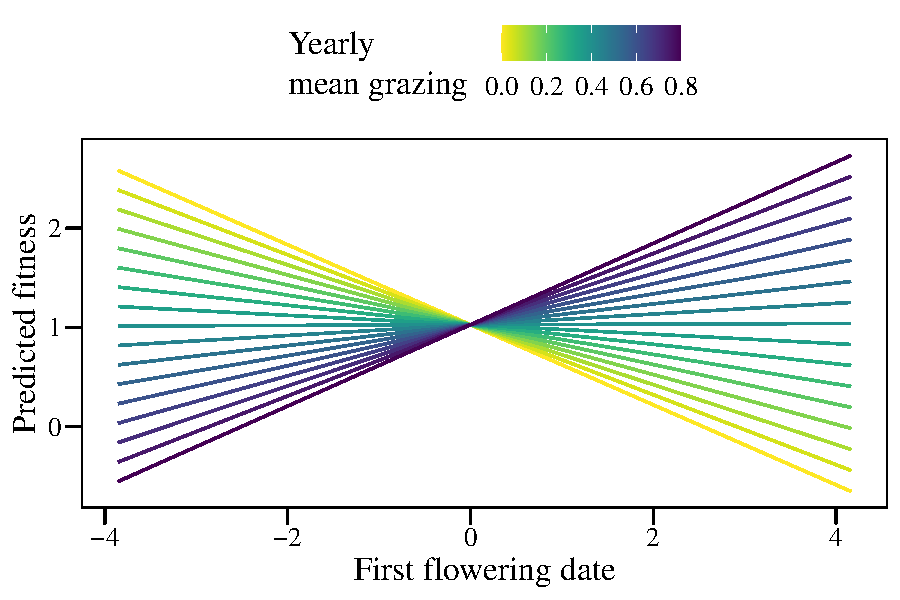
\includegraphics{lathyrus_ms3_3_after_rev_Ecology_files/figure-latex/unnamed-chunk-69-1.pdf}

\begin{Shaded}
\begin{Highlighting}[]
\KeywordTok{ggsave}\NormalTok{(}\DataTypeTok{filename=}\StringTok{"output/figures/AppendixS1\_2.tiff"}\NormalTok{,}
       \DataTypeTok{device=}\StringTok{"tiff"}\NormalTok{,}\DataTypeTok{width=}\DecValTok{25}\NormalTok{,}\DataTypeTok{height=}\DecValTok{10}\NormalTok{,}\DataTypeTok{units=}\StringTok{"cm"}\NormalTok{,}\DataTypeTok{dpi=}\DecValTok{300}\NormalTok{,}\DataTypeTok{compression=}\StringTok{"lzw"}\NormalTok{)}
\end{Highlighting}
\end{Shaded}

\hypertarget{fig.-s3}{%
\subsubsection{Fig. S3}\label{fig.-s3}}

\begin{Shaded}
\begin{Highlighting}[]
\CommentTok{\# Temperatures}
\NormalTok{weather\_all\textless{}{-}}\KeywordTok{read.table}\NormalTok{(}\StringTok{"data/weather.csv"}\NormalTok{,}
                    \DataTypeTok{header=}\NormalTok{T,}\DataTypeTok{sep=}\StringTok{"}\CharTok{\textbackslash{}t}\StringTok{"}\NormalTok{,}\DataTypeTok{dec=}\StringTok{"."}\NormalTok{) }

\KeywordTok{summarySE}\NormalTok{(}\KeywordTok{subset}\NormalTok{(}\KeywordTok{subset}\NormalTok{(weather\_all,year}\OperatorTok{\textgreater{}}\DecValTok{1986}\NormalTok{),}
\NormalTok{                 month}\OperatorTok{==}\DecValTok{3}\OperatorTok{|}\NormalTok{month}\OperatorTok{==}\DecValTok{4}\OperatorTok{|}\NormalTok{month}\OperatorTok{==}\DecValTok{5}\OperatorTok{|}\NormalTok{month}\OperatorTok{==}\DecValTok{6}\NormalTok{), }
          \DataTypeTok{measurevar=}\StringTok{"mean"}\NormalTok{, }\DataTypeTok{groupvars=}\KeywordTok{c}\NormalTok{(}\StringTok{"year"}\NormalTok{,}\StringTok{"month"}\NormalTok{))}\OperatorTok{\%\textgreater{}\%}
\StringTok{  }\KeywordTok{mutate}\NormalTok{(}\DataTypeTok{incl=}\KeywordTok{factor}\NormalTok{(}\KeywordTok{ifelse}\NormalTok{(year}\OperatorTok{==}\DecValTok{1995}\NormalTok{,}\DecValTok{0}\NormalTok{,}\KeywordTok{ifelse}\NormalTok{(year}\OperatorTok{\textgreater{}}\DecValTok{1996}\OperatorTok{\&}\NormalTok{year}\OperatorTok{\textless{}}\DecValTok{2006}\NormalTok{,}\DecValTok{0}\NormalTok{,}\DecValTok{1}\NormalTok{))))}\OperatorTok{\%\textgreater{}\%}
\KeywordTok{ggplot}\NormalTok{(}\KeywordTok{aes}\NormalTok{(}\DataTypeTok{x=}\NormalTok{year, }\DataTypeTok{y=}\NormalTok{mean, }\DataTypeTok{colour=}\KeywordTok{factor}\NormalTok{(month),}\DataTypeTok{ymin=}\NormalTok{mean}\OperatorTok{{-}}\NormalTok{se, }\DataTypeTok{ymax=}\NormalTok{mean}\OperatorTok{+}\NormalTok{se))}\OperatorTok{+}
\StringTok{  }\KeywordTok{geom\_errorbar}\NormalTok{(}\DataTypeTok{width=}\NormalTok{.}\DecValTok{3}\NormalTok{, }\DataTypeTok{position =} \KeywordTok{position\_dodge}\NormalTok{(}\DataTypeTok{width =} \FloatTok{0.5}\NormalTok{))}\OperatorTok{+}
\StringTok{  }\KeywordTok{geom\_line}\NormalTok{(}\DataTypeTok{position =} \KeywordTok{position\_dodge}\NormalTok{(}\DataTypeTok{width =} \FloatTok{0.5}\NormalTok{))}\OperatorTok{+}
\StringTok{  }\KeywordTok{geom\_point}\NormalTok{(}\KeywordTok{aes}\NormalTok{(}\DataTypeTok{shape=}\NormalTok{incl),}\DataTypeTok{size=}\DecValTok{5}\NormalTok{,}\DataTypeTok{position =} \KeywordTok{position\_dodge}\NormalTok{(}\DataTypeTok{width =} \FloatTok{0.5}\NormalTok{))}\OperatorTok{+}
\StringTok{  }\KeywordTok{xlab}\NormalTok{(}\StringTok{"Year"}\NormalTok{)}\OperatorTok{+}\KeywordTok{ylab}\NormalTok{(}\StringTok{"Mean daily temperature (ºC)"}\NormalTok{)}\OperatorTok{+}
\StringTok{  }\KeywordTok{my\_theme\_legend}\NormalTok{()}\OperatorTok{+}
\StringTok{  }\KeywordTok{scale\_fill\_manual}\NormalTok{(}\DataTypeTok{values=}\KeywordTok{c}\NormalTok{(}\StringTok{"\#E69F00"}\NormalTok{, }\StringTok{"\#56B4E9"}\NormalTok{, }\StringTok{"\#009E73"}\NormalTok{, }\StringTok{"\#F0E442"}\NormalTok{),}
                    \DataTypeTok{name=}\StringTok{"Month"}\NormalTok{,}\DataTypeTok{labels=}\KeywordTok{c}\NormalTok{(}\StringTok{"March"}\NormalTok{,}\StringTok{"April"}\NormalTok{,}\StringTok{"May"}\NormalTok{,}\StringTok{"June"}\NormalTok{))}\OperatorTok{+}
\StringTok{  }\KeywordTok{scale\_color\_manual}\NormalTok{(}\DataTypeTok{values=}\KeywordTok{c}\NormalTok{(}\StringTok{"\#E69F00"}\NormalTok{, }\StringTok{"\#56B4E9"}\NormalTok{, }\StringTok{"\#009E73"}\NormalTok{, }\StringTok{"\#F0E442"}\NormalTok{),}
                     \DataTypeTok{name=}\StringTok{"Month"}\NormalTok{,}\DataTypeTok{labels=}\KeywordTok{c}\NormalTok{(}\StringTok{"March"}\NormalTok{,}\StringTok{"April"}\NormalTok{,}\StringTok{"May"}\NormalTok{,}\StringTok{"June"}\NormalTok{))}\OperatorTok{+}
\StringTok{  }\KeywordTok{scale\_shape\_manual}\NormalTok{(}\DataTypeTok{values=}\KeywordTok{c}\NormalTok{(}\DecValTok{21}\NormalTok{,}\DecValTok{19}\NormalTok{),}\DataTypeTok{guide =} \OtherTok{FALSE}\NormalTok{)}\OperatorTok{+}
\StringTok{  }\KeywordTok{scale\_x\_continuous}\NormalTok{(}\DataTypeTok{breaks=}\KeywordTok{seq}\NormalTok{(}\DecValTok{1987}\NormalTok{,}\DecValTok{2017}\NormalTok{,}\DecValTok{1}\NormalTok{))}\OperatorTok{+}
\StringTok{  }\KeywordTok{theme}\NormalTok{(}\DataTypeTok{legend.position =} \KeywordTok{c}\NormalTok{(}\FloatTok{0.93}\NormalTok{, }\FloatTok{0.15}\NormalTok{))}
\end{Highlighting}
\end{Shaded}

\includegraphics{lathyrus_ms3_3_after_rev_Ecology_files/figure-latex/unnamed-chunk-70-1.pdf}

\begin{Shaded}
\begin{Highlighting}[]
\KeywordTok{ggsave}\NormalTok{(}\DataTypeTok{filename=}\StringTok{"output/figures/AppendixS1\_3.tiff"}\NormalTok{,}
       \DataTypeTok{device=}\StringTok{"tiff"}\NormalTok{,}\DataTypeTok{width=}\DecValTok{350}\NormalTok{,}\DataTypeTok{height=}\DecValTok{190}\NormalTok{,}\DataTypeTok{units=}\StringTok{"mm"}\NormalTok{,}\DataTypeTok{dpi=}\DecValTok{300}\NormalTok{,}\DataTypeTok{compression=}\StringTok{"lzw"}\NormalTok{)}
\end{Highlighting}
\end{Shaded}

\hypertarget{fig.-s4}{%
\subsubsection{Fig. S4}\label{fig.-s4}}

\begin{Shaded}
\begin{Highlighting}[]
\CommentTok{\# Interactions}
\NormalTok{S1\_}\DecValTok{4}\NormalTok{\textless{}{-}}\KeywordTok{grid.arrange}\NormalTok{(}
  \KeywordTok{ggplot}\NormalTok{(}\KeywordTok{summarySE}\NormalTok{(data\_selag,}\DataTypeTok{measurevar=}\StringTok{"grazing\_corr"}\NormalTok{,}
                   \DataTypeTok{groupvars=}\StringTok{"year"}\NormalTok{,}\DataTypeTok{na.rm=}\NormalTok{T),}
         \KeywordTok{aes}\NormalTok{(}\DataTypeTok{x=}\KeywordTok{factor}\NormalTok{(year),}\DataTypeTok{y=}\NormalTok{grazing\_corr))}\OperatorTok{+}\KeywordTok{geom\_point}\NormalTok{(}\DataTypeTok{size=}\DecValTok{3}\NormalTok{)}\OperatorTok{+}
\StringTok{    }\KeywordTok{geom\_errorbar}\NormalTok{(}\KeywordTok{aes}\NormalTok{(}\DataTypeTok{ymin=}\NormalTok{grazing\_corr}\OperatorTok{{-}}\NormalTok{se,}\DataTypeTok{ymax=}\NormalTok{grazing\_corr}\OperatorTok{+}\NormalTok{se),}
                  \DataTypeTok{width=}\NormalTok{.}\DecValTok{3}\NormalTok{)}\OperatorTok{+}
\StringTok{    }\KeywordTok{xlab}\NormalTok{(}\StringTok{"Year"}\NormalTok{)}\OperatorTok{+}\KeywordTok{ylab}\NormalTok{(}\StringTok{"Grazing"}\NormalTok{)}\OperatorTok{+}\KeywordTok{my\_theme}\NormalTok{()}\OperatorTok{+}\KeywordTok{ggtitle}\NormalTok{(}\StringTok{"A)"}\NormalTok{),}
  \KeywordTok{ggplot}\NormalTok{(}\KeywordTok{summarySE}\NormalTok{(data\_selag,}\DataTypeTok{measurevar=}\StringTok{"prop\_pred\_seeds"}\NormalTok{,}
                   \DataTypeTok{groupvars=}\StringTok{"year"}\NormalTok{,}\DataTypeTok{na.rm=}\NormalTok{T),}
         \KeywordTok{aes}\NormalTok{(}\DataTypeTok{x=}\KeywordTok{factor}\NormalTok{(year),}\DataTypeTok{y=}\NormalTok{prop\_pred\_seeds))}\OperatorTok{+}\KeywordTok{geom\_point}\NormalTok{(}\DataTypeTok{size=}\DecValTok{3}\NormalTok{)}\OperatorTok{+}
\StringTok{    }\KeywordTok{geom\_errorbar}\NormalTok{(}\KeywordTok{aes}\NormalTok{(}\DataTypeTok{ymin=}\NormalTok{prop\_pred\_seeds}\OperatorTok{{-}}\NormalTok{se,}\DataTypeTok{ymax=}\NormalTok{prop\_pred\_seeds}\OperatorTok{+}\NormalTok{se),}
                  \DataTypeTok{width=}\NormalTok{.}\DecValTok{3}\NormalTok{)}\OperatorTok{+}
\StringTok{    }\KeywordTok{xlab}\NormalTok{(}\StringTok{"Year"}\NormalTok{)}\OperatorTok{+}\KeywordTok{ylab}\NormalTok{(}\StringTok{"Seed predation"}\NormalTok{)}\OperatorTok{+}\KeywordTok{my\_theme}\NormalTok{()}\OperatorTok{+}\KeywordTok{ggtitle}\NormalTok{(}\StringTok{"B)"}\NormalTok{),}
  \DataTypeTok{ncol=}\DecValTok{1}\NormalTok{)}
\end{Highlighting}
\end{Shaded}

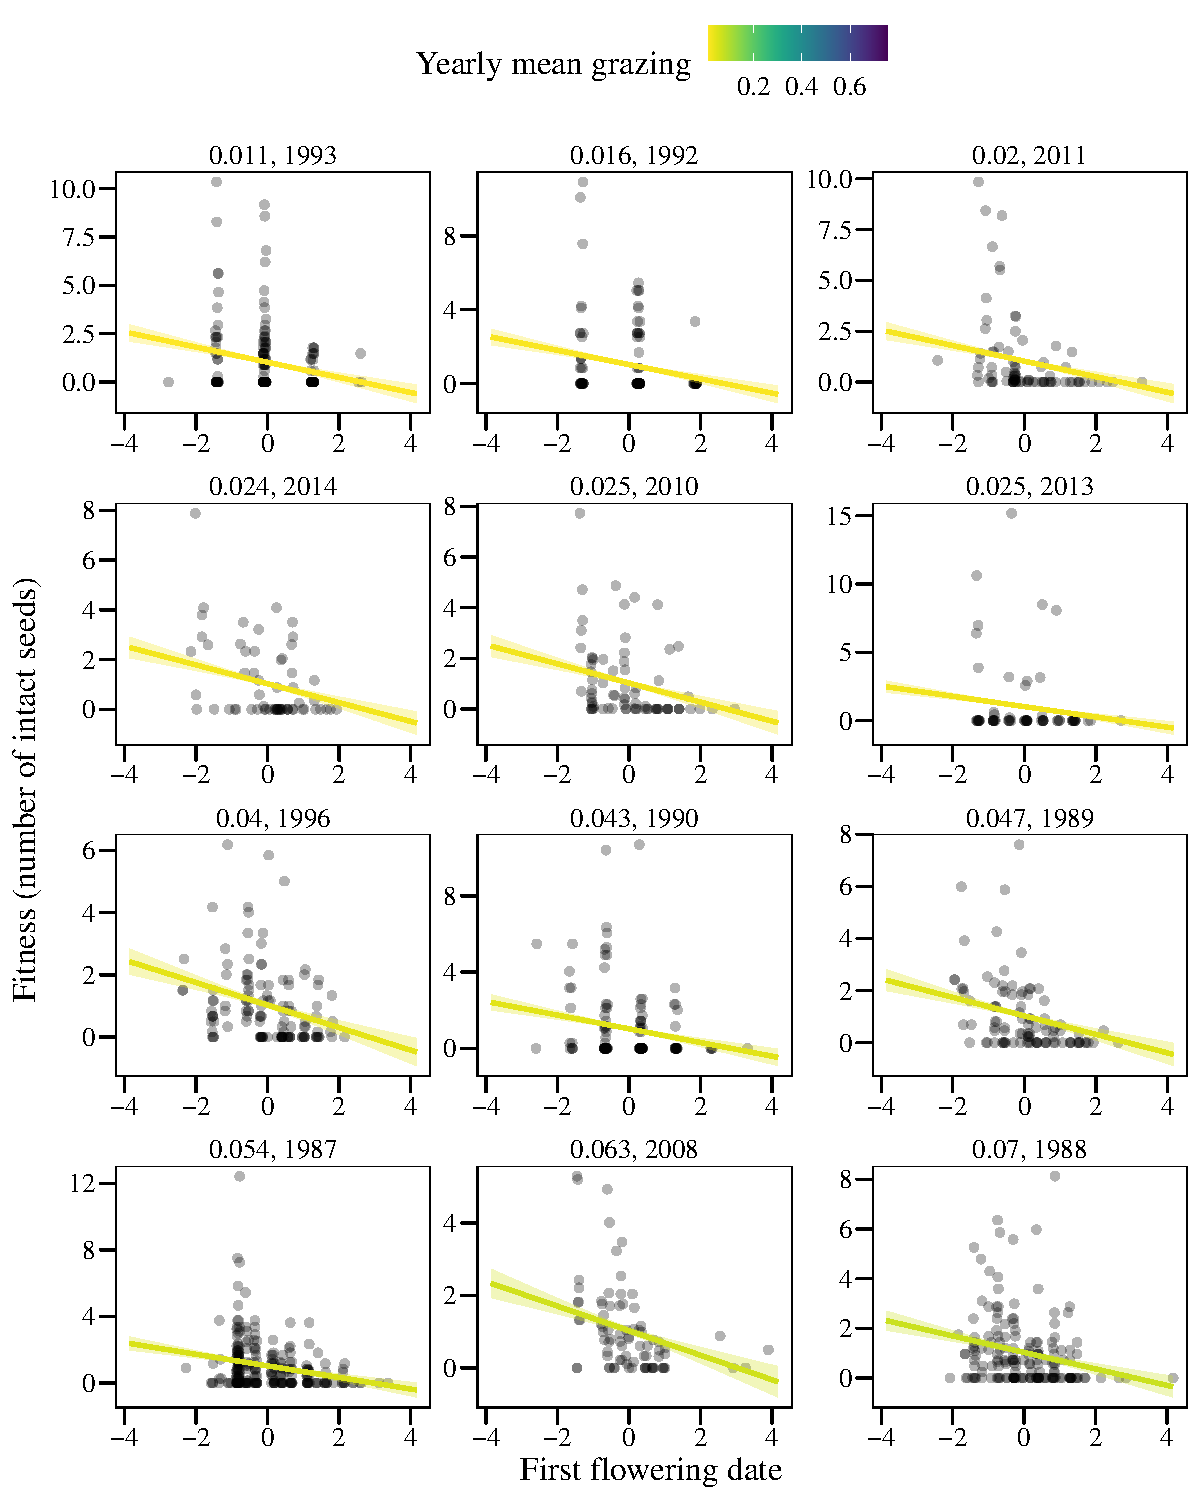
\includegraphics{lathyrus_ms3_3_after_rev_Ecology_files/figure-latex/unnamed-chunk-71-1.pdf}

\begin{Shaded}
\begin{Highlighting}[]
\KeywordTok{ggsave}\NormalTok{(}\DataTypeTok{filename=}\StringTok{"output/figures/AppendixS1\_4.tiff"}\NormalTok{,}\DataTypeTok{plot=}\NormalTok{S1\_}\DecValTok{4}\NormalTok{,}\DataTypeTok{device=}\StringTok{"tiff"}
\NormalTok{       ,}\DataTypeTok{width=}\DecValTok{25}\NormalTok{,}\DataTypeTok{height=}\DecValTok{20}\NormalTok{,}\DataTypeTok{units=}\StringTok{"cm"}\NormalTok{,}\DataTypeTok{dpi=}\DecValTok{300}\NormalTok{,}\DataTypeTok{compression=}\StringTok{"lzw"}\NormalTok{)}
\end{Highlighting}
\end{Shaded}

\hypertarget{appendix-s2-raw-relationships-biotic-interactions-ffd-in-different-years}{%
\section{Appendix S2: Raw relationships biotic interactions
\textasciitilde{} FFD in different
years}\label{appendix-s2-raw-relationships-biotic-interactions-ffd-in-different-years}}

\hypertarget{fig.-s1-raw-relationships-grazing-ffd-in-different-years}{%
\subsection{Fig. S1: Raw relationships grazing \textasciitilde{} FFD in
different
years}\label{fig.-s1-raw-relationships-grazing-ffd-in-different-years}}

\includegraphics{lathyrus_ms3_3_after_rev_Ecology_files/figure-latex/unnamed-chunk-72-1.pdf}
\includegraphics{lathyrus_ms3_3_after_rev_Ecology_files/figure-latex/unnamed-chunk-72-2.pdf}

See which models are significant and add asterisks in Inkscape.

\begin{Shaded}
\begin{Highlighting}[]
\NormalTok{data\_selag}\OperatorTok{\%\textgreater{}\%}
\StringTok{  }\KeywordTok{group\_by}\NormalTok{(year)}\OperatorTok{\%\textgreater{}\%}
\StringTok{  }\KeywordTok{do}\NormalTok{(}\DataTypeTok{models =} \KeywordTok{tidy}\NormalTok{(}\KeywordTok{glm}\NormalTok{(}\KeywordTok{cbind}\NormalTok{(grazing\_success,grazing\_failure)}\OperatorTok{\textasciitilde{}}\NormalTok{FFD,}
                       \DataTypeTok{family=}\StringTok{"binomial"}\NormalTok{, }\DataTypeTok{data =}\NormalTok{ .))) }\OperatorTok{\%\textgreater{}\%}\StringTok{ }
\StringTok{  }\KeywordTok{unnest}\NormalTok{(models)}\OperatorTok{\%\textgreater{}\%}
\StringTok{  }\KeywordTok{kable}\NormalTok{()}
\end{Highlighting}
\end{Shaded}

\begin{longtable}[]{@{}rlrrrr@{}}
\toprule
year & term & estimate & std.error & statistic & p.value\tabularnewline
\midrule
\endhead
1987 & (Intercept) & 1.7298398 & 1.7265416 & 1.0019103 &
0.3163869\tabularnewline
1987 & FFD & -0.0700661 & 0.0268897 & -2.6056885 &
0.0091690\tabularnewline
1988 & (Intercept) & 1.9719086 & 1.1528917 & 1.7104024 &
0.0871915\tabularnewline
1988 & FFD & -0.0700870 & 0.0200769 & -3.4909340 &
0.0004813\tabularnewline
1989 & (Intercept) & -5.4673744 & 1.9493721 & -2.8046849 &
0.0050366\tabularnewline
1989 & FFD & 0.0421013 & 0.0372304 & 1.1308331 &
0.2581254\tabularnewline
1990 & (Intercept) & 6.3951626 & 1.7621030 & 3.6292786 &
0.0002842\tabularnewline
1990 & FFD & -0.1838625 & 0.0353067 & -5.2075788 &
0.0000002\tabularnewline
1991 & (Intercept) & -2.1117549 & 1.1586807 & -1.8225511 &
0.0683714\tabularnewline
1991 & FFD & -0.0079446 & 0.0188172 & -0.4221972 &
0.6728811\tabularnewline
1992 & (Intercept) & -12.8019026 & 4.1030210 & -3.1201163 &
0.0018078\tabularnewline
1992 & FFD & 0.1571611 & 0.0682541 & 2.3025897 &
0.0213019\tabularnewline
1993 & (Intercept) & 9.3733831 & 4.9366747 & 1.8987241 &
0.0576008\tabularnewline
1993 & FFD & -0.2583564 & 0.0944311 & -2.7359232 &
0.0062206\tabularnewline
1994 & (Intercept) & 9.0739724 & 1.1544258 & 7.8601605 &
0.0000000\tabularnewline
1994 & FFD & -0.1774131 & 0.0200920 & -8.8300497 &
0.0000000\tabularnewline
1996 & (Intercept) & 8.6569004 & 1.6474675 & 5.2546713 &
0.0000001\tabularnewline
1996 & FFD & -0.1574730 & 0.0244294 & -6.4460348 &
0.0000000\tabularnewline
2006 & (Intercept) & 6.9581121 & 3.1134861 & 2.2348300 &
0.0254285\tabularnewline
2006 & FFD & -0.1474856 & 0.0547639 & -2.6931181 &
0.0070787\tabularnewline
2007 & (Intercept) & -6.9283713 & 0.0780109 & -88.8129084 &
0.0000000\tabularnewline
2007 & FFD & 0.0843498 & 0.0015185 & 55.5496819 &
0.0000000\tabularnewline
2008 & (Intercept) & -3.4960048 & 0.0777449 & -44.9676306 &
0.0000000\tabularnewline
2008 & FFD & 0.0123529 & 0.0016695 & 7.3989725 &
0.0000000\tabularnewline
2009 & (Intercept) & 8.4126247 & 0.1972684 & 42.6455776 &
0.0000000\tabularnewline
2009 & FFD & -0.2116604 & 0.0037712 & -56.1253985 &
0.0000000\tabularnewline
2010 & (Intercept) & 0.6854620 & 0.3156545 & 2.1715581 &
0.0298890\tabularnewline
2010 & FFD & -0.0746027 & 0.0055393 & -13.4678878 &
0.0000000\tabularnewline
2011 & (Intercept) & -0.5667847 & 0.2371127 & -2.3903602 &
0.0168319\tabularnewline
2011 & FFD & -0.0677340 & 0.0046937 & -14.4307908 &
0.0000000\tabularnewline
2012 & (Intercept) & -5.9297569 & 0.1530281 & -38.7494755 &
0.0000000\tabularnewline
2012 & FFD & 0.0510410 & 0.0027858 & 18.3216027 &
0.0000000\tabularnewline
2013 & (Intercept) & -44.7399188 & 2.8030402 & -15.9612121 &
0.0000000\tabularnewline
2013 & FFD & 0.6240086 & 0.0447759 & 13.9362460 &
0.0000000\tabularnewline
2014 & (Intercept) & -5.7477342 & 0.1806441 & -31.8179982 &
0.0000000\tabularnewline
2014 & FFD & 0.0451589 & 0.0033236 & 13.5872239 &
0.0000000\tabularnewline
2015 & (Intercept) & 5.8696540 & 0.1242426 & 47.2434868 &
0.0000000\tabularnewline
2015 & FFD & -0.1391928 & 0.0025598 & -54.3765351 &
0.0000000\tabularnewline
2016 & (Intercept) & -0.3726617 & 0.9492031 & -0.3926049 &
0.6946113\tabularnewline
2016 & FFD & -0.0156003 & 0.0187671 & -0.8312612 &
0.4058261\tabularnewline
2017 & (Intercept) & 28.6595716 & 1.8855876 & 15.1992790 &
0.0000000\tabularnewline
2017 & FFD & -0.4504012 & 0.0313242 & -14.3787215 &
0.0000000\tabularnewline
\bottomrule
\end{longtable}

\hypertarget{fig.-s2-raw-relationships-predation-ffd-in-different-years}{%
\subsection{Fig. S2: Raw relationships predation \textasciitilde{} FFD
in different
years}\label{fig.-s2-raw-relationships-predation-ffd-in-different-years}}

\includegraphics{lathyrus_ms3_3_after_rev_Ecology_files/figure-latex/unnamed-chunk-74-1.pdf}
\includegraphics{lathyrus_ms3_3_after_rev_Ecology_files/figure-latex/unnamed-chunk-74-2.pdf}

See which models are significant and add asterisks in Inkscape.

\begin{Shaded}
\begin{Highlighting}[]
\NormalTok{data\_selag}\OperatorTok{\%\textgreater{}\%}
\StringTok{  }\KeywordTok{group\_by}\NormalTok{(year)}\OperatorTok{\%\textgreater{}\%}
\StringTok{  }\KeywordTok{do}\NormalTok{(}\DataTypeTok{models =} \KeywordTok{tidy}\NormalTok{(}\KeywordTok{glm}\NormalTok{(}\KeywordTok{cbind}\NormalTok{(}\KeywordTok{round}\NormalTok{(n\_pred\_seeds),}\KeywordTok{round}\NormalTok{(n\_intact\_seeds))}\OperatorTok{\textasciitilde{}}\NormalTok{FFD,}
                       \DataTypeTok{family=}\StringTok{"binomial"}\NormalTok{, }\DataTypeTok{data =}\NormalTok{ .))) }\OperatorTok{\%\textgreater{}\%}\StringTok{ }
\StringTok{  }\KeywordTok{unnest}\NormalTok{(models)}\OperatorTok{\%\textgreater{}\%}
\StringTok{  }\KeywordTok{kable}\NormalTok{()}
\end{Highlighting}
\end{Shaded}

\begin{longtable}[]{@{}rlrrrr@{}}
\toprule
year & term & estimate & std.error & statistic & p.value\tabularnewline
\midrule
\endhead
1987 & (Intercept) & 14.5914443 & 1.8932985 & 7.7068907 &
0.0000000\tabularnewline
1987 & FFD & -0.2552723 & 0.0298671 & -8.5469528 &
0.0000000\tabularnewline
1988 & (Intercept) & 4.9009502 & 0.8829805 & 5.5504625 &
0.0000000\tabularnewline
1988 & FFD & -0.0846898 & 0.0152032 & -5.5705433 &
0.0000000\tabularnewline
1989 & (Intercept) & 0.4825583 & 1.0738329 & 0.4493793 &
0.6531580\tabularnewline
1989 & FFD & -0.0333720 & 0.0210332 & -1.5866373 &
0.1125948\tabularnewline
1990 & (Intercept) & 0.9192979 & 1.1187335 & 0.8217309 &
0.4112301\tabularnewline
1990 & FFD & -0.0387113 & 0.0216220 & -1.7903658 &
0.0733951\tabularnewline
1991 & (Intercept) & 1.5640487 & 2.5356827 & 0.6168156 &
0.5373563\tabularnewline
1991 & FFD & -0.0839246 & 0.0423937 & -1.9796503 &
0.0477428\tabularnewline
1992 & (Intercept) & -1.5474373 & 2.2382052 & -0.6913742 &
0.4893304\tabularnewline
1992 & FFD & 0.0366799 & 0.0381887 & 0.9604924 &
0.3368075\tabularnewline
1993 & (Intercept) & -5.6281413 & 1.3644633 & -4.1248024 &
0.0000371\tabularnewline
1993 & FFD & 0.0827068 & 0.0248576 & 3.3272182 &
0.0008772\tabularnewline
1994 & (Intercept) & 9.6238162 & 1.7253215 & 5.5779843 &
0.0000000\tabularnewline
1994 & FFD & -0.1803155 & 0.0306599 & -5.8811461 &
0.0000000\tabularnewline
1996 & (Intercept) & -1.2479616 & 1.3246503 & -0.9421065 &
0.3461381\tabularnewline
1996 & FFD & -0.0040214 & 0.0189923 & -0.2117381 &
0.8323114\tabularnewline
2006 & (Intercept) & -3.3681119 & 1.0059408 & -3.3482209 &
0.0008133\tabularnewline
2006 & FFD & 0.0589115 & 0.0176106 & 3.3452294 &
0.0008221\tabularnewline
2007 & (Intercept) & 1.8073422 & 0.5047317 & 3.5807979 &
0.0003425\tabularnewline
2007 & FFD & -0.0309006 & 0.0102960 & -3.0012147 &
0.0026890\tabularnewline
2008 & (Intercept) & -0.2696102 & 0.6544337 & -0.4119749 &
0.6803578\tabularnewline
2008 & FFD & -0.0270508 & 0.0145778 & -1.8556150 &
0.0635085\tabularnewline
2009 & (Intercept) & 7.9679981 & 1.8747463 & 4.2501740 &
0.0000214\tabularnewline
2009 & FFD & -0.1291403 & 0.0344679 & -3.7466810 &
0.0001792\tabularnewline
2010 & (Intercept) & 6.7275171 & 1.9860185 & 3.3874393 &
0.0007055\tabularnewline
2010 & FFD & -0.0953435 & 0.0348624 & -2.7348544 &
0.0062408\tabularnewline
2011 & (Intercept) & 1.6615835 & 2.1109697 & 0.7871186 &
0.4312125\tabularnewline
2011 & FFD & 0.0069380 & 0.0422224 & 0.1643205 &
0.8694788\tabularnewline
2012 & (Intercept) & -18.4312933 & 1.7113995 & -10.7697197 &
0.0000000\tabularnewline
2012 & FFD & 0.3514273 & 0.0326561 & 10.7614541 &
0.0000000\tabularnewline
2013 & (Intercept) & -12.1954335 & 7.1493843 & -1.7058019 &
0.0880450\tabularnewline
2013 & FFD & 0.2197089 & 0.1216523 & 1.8060398 &
0.0709121\tabularnewline
2014 & (Intercept) & -7.5927635 & 2.0322217 & -3.7361886 &
0.0001868\tabularnewline
2014 & FFD & 0.1013409 & 0.0375298 & 2.7002760 &
0.0069282\tabularnewline
2015 & (Intercept) & -17.4819210 & 10.1969190 & -1.7144317 &
0.0864495\tabularnewline
2015 & FFD & 0.2335959 & 0.1754076 & 1.3317319 &
0.1829483\tabularnewline
2016 & (Intercept) & -2.3869026 & 0.8965040 & -2.6624561 &
0.0077573\tabularnewline
2016 & FFD & 0.0281622 & 0.0175015 & 1.6091287 &
0.1075882\tabularnewline
2017 & (Intercept) & 13.4648958 & 8.6097719 & 1.5639086 &
0.1178390\tabularnewline
2017 & FFD & -0.2192434 & 0.1434799 & -1.5280431 &
0.1265018\tabularnewline
\bottomrule
\end{longtable}

\hypertarget{appendix-s3-variation-in-the-relationships-among-interaction-intensities-and-individual-flowering-time-among-years}{%
\section{Appendix S3: Variation in the relationships among interaction
intensities and individual flowering time among
years}\label{appendix-s3-variation-in-the-relationships-among-interaction-intensities-and-individual-flowering-time-among-years}}

Table: Models with interaction FFD x year

\begin{Shaded}
\begin{Highlighting}[]
\NormalTok{graz\_FFD\_yrs\textless{}{-}}\KeywordTok{glmmTMB}\NormalTok{(}\KeywordTok{cbind}\NormalTok{(grazing\_success,grazing\_failure)}\OperatorTok{\textasciitilde{}}
\StringTok{                        }\NormalTok{FFD}\OperatorTok{*}\KeywordTok{as.factor}\NormalTok{(year)}\OperatorTok{+}\NormalTok{(}\DecValTok{1}\OperatorTok{|}\NormalTok{id),}
                      \DataTypeTok{data =}\NormalTok{ data\_selag,}\DataTypeTok{family=}\StringTok{"betabinomial"}\NormalTok{)}
\KeywordTok{Anova}\NormalTok{(graz\_FFD\_yrs)}
\end{Highlighting}
\end{Shaded}

\begin{verbatim}
## Analysis of Deviance Table (Type II Wald chisquare tests)
## 
## Response: cbind(grazing_success, grazing_failure)
##                       Chisq Df Pr(>Chisq)    
## FFD                  21.764  1  3.083e-06 ***
## as.factor(year)     257.726 20  < 2.2e-16 ***
## FFD:as.factor(year)  57.191 20  1.920e-05 ***
## ---
## Signif. codes:  0 '***' 0.001 '**' 0.01 '*' 0.05 '.' 0.1 ' ' 1
\end{verbatim}

\begin{Shaded}
\begin{Highlighting}[]
\NormalTok{pred\_FFD\_yrs\textless{}{-}}\KeywordTok{glmmTMB}\NormalTok{(}\KeywordTok{cbind}\NormalTok{(}\KeywordTok{round}\NormalTok{(n\_pred\_seeds),}\KeywordTok{round}\NormalTok{(n\_intact\_seeds))}\OperatorTok{\textasciitilde{}}
\StringTok{                        }\NormalTok{FFD}\OperatorTok{*}\KeywordTok{as.factor}\NormalTok{(year),}
                      \DataTypeTok{data=}\KeywordTok{subset}\NormalTok{(}\KeywordTok{subset}\NormalTok{(data\_selag,n\_seeds}\OperatorTok{\textgreater{}}\DecValTok{0}\NormalTok{),}
                                  \OperatorTok{!}\KeywordTok{is.na}\NormalTok{(n\_intact\_seeds)),}\DataTypeTok{family=}\StringTok{"betabinomial"}\NormalTok{)}
\KeywordTok{Anova}\NormalTok{(pred\_FFD\_yrs)}
\end{Highlighting}
\end{Shaded}

\begin{verbatim}
## Analysis of Deviance Table (Type II Wald chisquare tests)
## 
## Response: cbind(round(n_pred_seeds), round(n_intact_seeds))
##                        Chisq Df Pr(>Chisq)    
## FFD                   0.3098  1  0.5777766    
## as.factor(year)     603.4516 20  < 2.2e-16 ***
## FFD:as.factor(year)  52.1063 20  0.0001099 ***
## ---
## Signif. codes:  0 '***' 0.001 '**' 0.01 '*' 0.05 '.' 0.1 ' ' 1
\end{verbatim}

\hypertarget{appendix-s4relationships-between-temperatures-and-predicted-seed-predation-for-different-parts-of-the-distribution-of-flowering-dates}{%
\section{Appendix S4:Relationships between temperatures and predicted
seed predation for different parts of the distribution of flowering
dates}\label{appendix-s4relationships-between-temperatures-and-predicted-seed-predation-for-different-parts-of-the-distribution-of-flowering-dates}}

\begin{Shaded}
\begin{Highlighting}[]
\KeywordTok{mean}\NormalTok{(}\KeywordTok{subset}\NormalTok{(data\_selag,n\_seeds}\OperatorTok{\textgreater{}}\DecValTok{0}\OperatorTok{\&}\NormalTok{FFD\_s\_y}\OperatorTok{\textless{}={-}}\FloatTok{0.84}\NormalTok{)}\OperatorTok{$}\NormalTok{FFD\_s\_y) }
\end{Highlighting}
\end{Shaded}

\begin{verbatim}
## [1] -1.247518
\end{verbatim}

\begin{Shaded}
\begin{Highlighting}[]
\CommentTok{\# Mean cat 1 = {-}1.247518}
\KeywordTok{mean}\NormalTok{(}\KeywordTok{subset}\NormalTok{(data\_selag,n\_seeds}\OperatorTok{\textgreater{}}\DecValTok{0}\OperatorTok{\&}\NormalTok{FFD\_s\_y}\OperatorTok{\textgreater{}{-}}\FloatTok{0.84}\OperatorTok{\&}\NormalTok{FFD\_s\_y}\OperatorTok{\textless{}={-}}\FloatTok{0.28}\NormalTok{)}\OperatorTok{$}\NormalTok{FFD\_s\_y) }
\end{Highlighting}
\end{Shaded}

\begin{verbatim}
## [1] -0.5992093
\end{verbatim}

\begin{Shaded}
\begin{Highlighting}[]
\CommentTok{\# Mean cat 2 = {-}0.5992093}
\KeywordTok{mean}\NormalTok{(}\KeywordTok{subset}\NormalTok{(data\_selag,n\_seeds}\OperatorTok{\textgreater{}}\DecValTok{0}\OperatorTok{\&}\NormalTok{FFD\_s\_y}\OperatorTok{\textgreater{}{-}}\FloatTok{0.28}\OperatorTok{\&}\NormalTok{FFD\_s\_y}\OperatorTok{\textless{}=}\FloatTok{0.26}\NormalTok{)}\OperatorTok{$}\NormalTok{FFD\_s\_y) }
\end{Highlighting}
\end{Shaded}

\begin{verbatim}
## [1] -0.008394325
\end{verbatim}

\begin{Shaded}
\begin{Highlighting}[]
\CommentTok{\# Mean cat 3 = {-}0.008394325}
\KeywordTok{mean}\NormalTok{(}\KeywordTok{subset}\NormalTok{(data\_selag,n\_seeds}\OperatorTok{\textgreater{}}\DecValTok{0}\OperatorTok{\&}\NormalTok{FFD\_s\_y}\OperatorTok{\textgreater{}}\FloatTok{0.16}\NormalTok{)}\OperatorTok{$}\NormalTok{FFD\_s\_y) }
\end{Highlighting}
\end{Shaded}

\begin{verbatim}
## [1] 0.7891997
\end{verbatim}

\begin{Shaded}
\begin{Highlighting}[]
\CommentTok{\# Mean cat 4 = 0.7891997}

\NormalTok{pred\_seedpred\_mean3\textless{}{-}}\KeywordTok{rbind}\NormalTok{(}
\NormalTok{  (}\KeywordTok{data.frame}\NormalTok{(}\KeywordTok{ggpredict}\NormalTok{(mod\_seedpred\_bb,}
                        \DataTypeTok{terms =} \KeywordTok{c}\NormalTok{(}\StringTok{"mean\_3 [all]"}\NormalTok{,}\StringTok{"FFD\_s\_y [{-}1.247518]"}\NormalTok{)))}\OperatorTok{\%\textgreater{}\%}
\StringTok{     }\KeywordTok{mutate}\NormalTok{(}\DataTypeTok{FFD\_s\_y\_cat=}\DecValTok{1}\NormalTok{)}\OperatorTok{\%\textgreater{}\%}
\StringTok{     }\NormalTok{dplyr}\OperatorTok{::}\KeywordTok{rename}\NormalTok{(}\DataTypeTok{temp=}\NormalTok{x, }\DataTypeTok{prop\_pred\_seeds=}\NormalTok{predicted,}\DataTypeTok{FFD\_s\_y=}\NormalTok{group)),}
\NormalTok{  (}\KeywordTok{data.frame}\NormalTok{(}\KeywordTok{ggpredict}\NormalTok{(mod\_seedpred\_bb,}
                        \DataTypeTok{terms =} \KeywordTok{c}\NormalTok{(}\StringTok{"mean\_3 [all]"}\NormalTok{,}\StringTok{"FFD\_s\_y [{-}0.5992093]"}\NormalTok{)))}\OperatorTok{\%\textgreater{}\%}
\StringTok{     }\KeywordTok{mutate}\NormalTok{(}\DataTypeTok{FFD\_s\_y\_cat=}\DecValTok{2}\NormalTok{)}\OperatorTok{\%\textgreater{}\%}
\StringTok{     }\NormalTok{dplyr}\OperatorTok{::}\KeywordTok{rename}\NormalTok{(}\DataTypeTok{temp=}\NormalTok{x, }\DataTypeTok{prop\_pred\_seeds=}\NormalTok{predicted,}\DataTypeTok{FFD\_s\_y=}\NormalTok{group)),}
\NormalTok{  (}\KeywordTok{data.frame}\NormalTok{(}\KeywordTok{ggpredict}\NormalTok{(mod\_seedpred\_bb,}
                        \DataTypeTok{terms =} \KeywordTok{c}\NormalTok{(}\StringTok{"mean\_3 [all]"}\NormalTok{,}\StringTok{"FFD\_s\_y [{-}0.008394325]"}\NormalTok{)))}\OperatorTok{\%\textgreater{}\%}
\StringTok{     }\KeywordTok{mutate}\NormalTok{(}\DataTypeTok{FFD\_s\_y\_cat=}\DecValTok{3}\NormalTok{)}\OperatorTok{\%\textgreater{}\%}
\StringTok{     }\NormalTok{dplyr}\OperatorTok{::}\KeywordTok{rename}\NormalTok{(}\DataTypeTok{temp=}\NormalTok{x, }\DataTypeTok{prop\_pred\_seeds=}\NormalTok{predicted,}\DataTypeTok{FFD\_s\_y=}\NormalTok{group)),}
\NormalTok{  (}\KeywordTok{data.frame}\NormalTok{(}\KeywordTok{ggpredict}\NormalTok{(mod\_seedpred\_bb,}
                        \DataTypeTok{terms =} \KeywordTok{c}\NormalTok{(}\StringTok{"mean\_3 [all]"}\NormalTok{,}\StringTok{"FFD\_s\_y [0.7891997]"}\NormalTok{)))}\OperatorTok{\%\textgreater{}\%}
\StringTok{     }\KeywordTok{mutate}\NormalTok{(}\DataTypeTok{FFD\_s\_y\_cat=}\DecValTok{4}\NormalTok{)}\OperatorTok{\%\textgreater{}\%}
\StringTok{     }\NormalTok{dplyr}\OperatorTok{::}\KeywordTok{rename}\NormalTok{(}\DataTypeTok{temp=}\NormalTok{x, }\DataTypeTok{prop\_pred\_seeds=}\NormalTok{predicted,}\DataTypeTok{FFD\_s\_y=}\NormalTok{group)))}\OperatorTok{\%\textgreater{}\%}
\StringTok{  }\KeywordTok{mutate}\NormalTok{(}\DataTypeTok{month=}\StringTok{"3"}\NormalTok{)}
\NormalTok{pred\_seedpred\_mean4\textless{}{-}}\KeywordTok{rbind}\NormalTok{(}
\NormalTok{  (}\KeywordTok{data.frame}\NormalTok{(}\KeywordTok{ggpredict}\NormalTok{(mod\_seedpred\_bb,}
                        \DataTypeTok{terms =} \KeywordTok{c}\NormalTok{(}\StringTok{"mean\_4 [all]"}\NormalTok{,}\StringTok{"FFD\_s\_y [{-}1.247518]"}\NormalTok{)))}\OperatorTok{\%\textgreater{}\%}
\StringTok{     }\KeywordTok{mutate}\NormalTok{(}\DataTypeTok{FFD\_s\_y\_cat=}\DecValTok{1}\NormalTok{)}\OperatorTok{\%\textgreater{}\%}
\StringTok{     }\NormalTok{dplyr}\OperatorTok{::}\KeywordTok{rename}\NormalTok{(}\DataTypeTok{temp=}\NormalTok{x, }\DataTypeTok{prop\_pred\_seeds=}\NormalTok{predicted,}\DataTypeTok{FFD\_s\_y=}\NormalTok{group)),}
\NormalTok{  (}\KeywordTok{data.frame}\NormalTok{(}\KeywordTok{ggpredict}\NormalTok{(mod\_seedpred\_bb,}
                        \DataTypeTok{terms =} \KeywordTok{c}\NormalTok{(}\StringTok{"mean\_4 [all]"}\NormalTok{,}\StringTok{"FFD\_s\_y [{-}0.5992093]"}\NormalTok{)))}\OperatorTok{\%\textgreater{}\%}
\StringTok{     }\KeywordTok{mutate}\NormalTok{(}\DataTypeTok{FFD\_s\_y\_cat=}\DecValTok{2}\NormalTok{)}\OperatorTok{\%\textgreater{}\%}
\StringTok{     }\NormalTok{dplyr}\OperatorTok{::}\KeywordTok{rename}\NormalTok{(}\DataTypeTok{temp=}\NormalTok{x, }\DataTypeTok{prop\_pred\_seeds=}\NormalTok{predicted,}\DataTypeTok{FFD\_s\_y=}\NormalTok{group)),}
\NormalTok{  (}\KeywordTok{data.frame}\NormalTok{(}\KeywordTok{ggpredict}\NormalTok{(mod\_seedpred\_bb,}
                        \DataTypeTok{terms =} \KeywordTok{c}\NormalTok{(}\StringTok{"mean\_4 [all]"}\NormalTok{,}\StringTok{"FFD\_s\_y [{-}0.008394325]"}\NormalTok{)))}\OperatorTok{\%\textgreater{}\%}
\StringTok{     }\KeywordTok{mutate}\NormalTok{(}\DataTypeTok{FFD\_s\_y\_cat=}\DecValTok{3}\NormalTok{)}\OperatorTok{\%\textgreater{}\%}
\StringTok{     }\NormalTok{dplyr}\OperatorTok{::}\KeywordTok{rename}\NormalTok{(}\DataTypeTok{temp=}\NormalTok{x, }\DataTypeTok{prop\_pred\_seeds=}\NormalTok{predicted,}\DataTypeTok{FFD\_s\_y=}\NormalTok{group)),}
\NormalTok{  (}\KeywordTok{data.frame}\NormalTok{(}\KeywordTok{ggpredict}\NormalTok{(mod\_seedpred\_bb,}
                        \DataTypeTok{terms =} \KeywordTok{c}\NormalTok{(}\StringTok{"mean\_4 [all]"}\NormalTok{,}\StringTok{"FFD\_s\_y [0.7891997]"}\NormalTok{)))}\OperatorTok{\%\textgreater{}\%}
\StringTok{     }\KeywordTok{mutate}\NormalTok{(}\DataTypeTok{FFD\_s\_y\_cat=}\DecValTok{4}\NormalTok{)}\OperatorTok{\%\textgreater{}\%}
\StringTok{     }\NormalTok{dplyr}\OperatorTok{::}\KeywordTok{rename}\NormalTok{(}\DataTypeTok{temp=}\NormalTok{x, }\DataTypeTok{prop\_pred\_seeds=}\NormalTok{predicted,}\DataTypeTok{FFD\_s\_y=}\NormalTok{group)))}\OperatorTok{\%\textgreater{}\%}
\StringTok{  }\KeywordTok{mutate}\NormalTok{(}\DataTypeTok{month=}\StringTok{"4"}\NormalTok{)}
\NormalTok{pred\_seedpred\textless{}{-}}\KeywordTok{rbind}\NormalTok{(pred\_seedpred\_mean3,pred\_seedpred\_mean4)}

\NormalTok{label\_names1 \textless{}{-}}\StringTok{ }\KeywordTok{list}\NormalTok{(}
  \StringTok{\textquotesingle{}1\textquotesingle{}}\NormalTok{=}\StringTok{"First quarter}\CharTok{\textbackslash{}n}\StringTok{Mean FFD = {-}1.25"}\NormalTok{,}
  \StringTok{\textquotesingle{}2\textquotesingle{}}\NormalTok{=}\StringTok{"Second quarter}\CharTok{\textbackslash{}n}\StringTok{Mean FFD = {-}0.60"}\NormalTok{,}
  \StringTok{\textquotesingle{}3\textquotesingle{}}\NormalTok{=}\StringTok{"Third quarter}\CharTok{\textbackslash{}n}\StringTok{Mean FFD = {-}0.01"}\NormalTok{,}
  \StringTok{\textquotesingle{}4\textquotesingle{}}\NormalTok{=}\StringTok{"Fourth quarter}\CharTok{\textbackslash{}n}\StringTok{Mean FFD = 0.79"}
\NormalTok{)}

\NormalTok{label\_names2 \textless{}{-}}\StringTok{ }\KeywordTok{list}\NormalTok{(}
  \StringTok{\textquotesingle{}3\textquotesingle{}}\NormalTok{=}\StringTok{"March"}\NormalTok{,}
  \StringTok{\textquotesingle{}4\textquotesingle{}}\NormalTok{=}\StringTok{"April"}
\NormalTok{)}

\NormalTok{labeller\_function1 \textless{}{-}}\StringTok{ }\ControlFlowTok{function}\NormalTok{(variable,value)\{}
  \KeywordTok{return}\NormalTok{(label\_names1[value])}
\NormalTok{\}}

\NormalTok{labeller\_function2 \textless{}{-}}\StringTok{ }\ControlFlowTok{function}\NormalTok{(variable,value)\{}
  \KeywordTok{return}\NormalTok{(label\_names2[value])}
\NormalTok{\}}
\end{Highlighting}
\end{Shaded}

\begin{Shaded}
\begin{Highlighting}[]
\KeywordTok{ggplot}\NormalTok{(}\KeywordTok{subset}\NormalTok{(data\_selag,n\_seeds}\OperatorTok{\textgreater{}}\DecValTok{0}\OperatorTok{\&!}\KeywordTok{is.na}\NormalTok{(FFD\_s\_y))}\OperatorTok{\%\textgreater{}\%}
\StringTok{         }\KeywordTok{ungroup}\NormalTok{()}\OperatorTok{\%\textgreater{}\%}
\StringTok{         }\CommentTok{\# Define 4 FFD\_s\_y categories based on quartiles}
\StringTok{         }\KeywordTok{mutate}\NormalTok{(}\DataTypeTok{FFD\_s\_y\_cat=}\KeywordTok{as.factor}\NormalTok{(}
           \KeywordTok{ifelse}\NormalTok{(FFD\_s\_y}\OperatorTok{\textless{}={-}}\FloatTok{0.84}\NormalTok{,}\DecValTok{1}\NormalTok{,}
                  \KeywordTok{ifelse}\NormalTok{(FFD\_s\_y}\OperatorTok{\textgreater{}{-}}\FloatTok{0.84}\OperatorTok{\&}\NormalTok{FFD\_s\_y}\OperatorTok{\textless{}={-}}\FloatTok{0.28}\NormalTok{,}\DecValTok{2}\NormalTok{,}
                         \KeywordTok{ifelse}\NormalTok{(FFD\_s\_y}\OperatorTok{\textgreater{}{-}}\FloatTok{0.28}\OperatorTok{\&}\NormalTok{FFD\_s\_y}\OperatorTok{\textless{}=}\FloatTok{0.26}\NormalTok{,}\DecValTok{3}\NormalTok{,}\DecValTok{4}\NormalTok{)))))}\OperatorTok{\%\textgreater{}\%}
\StringTok{         }\KeywordTok{select}\NormalTok{(mean\_}\DecValTok{3}\NormalTok{,mean\_}\DecValTok{4}\NormalTok{,prop\_pred\_seeds,FFD\_s\_y\_cat)}\OperatorTok{\%\textgreater{}\%}
\StringTok{         }\NormalTok{dplyr}\OperatorTok{::}\KeywordTok{rename}\NormalTok{(}\DataTypeTok{March=}\NormalTok{mean\_}\DecValTok{3}\NormalTok{,}\DataTypeTok{April=}\NormalTok{mean\_}\DecValTok{4}\NormalTok{)}\OperatorTok{\%\textgreater{}\%}
\StringTok{         }\KeywordTok{pivot\_longer}\NormalTok{(}\DataTypeTok{cols=}\NormalTok{March}\OperatorTok{:}\NormalTok{April,}\DataTypeTok{names\_to=}\StringTok{"month"}\NormalTok{,}\DataTypeTok{values\_to=}\StringTok{"temp"}\NormalTok{)}\OperatorTok{\%\textgreater{}\%}
\StringTok{         }\KeywordTok{mutate}\NormalTok{(}\DataTypeTok{month=}\KeywordTok{ifelse}\NormalTok{(month}\OperatorTok{==}\StringTok{"March"}\NormalTok{,}\DecValTok{3}\NormalTok{,}\DecValTok{4}\NormalTok{)),}
       \KeywordTok{aes}\NormalTok{(}\DataTypeTok{x=}\NormalTok{temp,}\DataTypeTok{y=}\NormalTok{prop\_pred\_seeds))}\OperatorTok{+}
\StringTok{  }\KeywordTok{facet\_grid}\NormalTok{(month}\OperatorTok{\textasciitilde{}}\NormalTok{FFD\_s\_y\_cat,}\DataTypeTok{scales=}\StringTok{"free"}\NormalTok{,}
             \DataTypeTok{labeller=}\KeywordTok{labeller}\NormalTok{(}\DataTypeTok{FFD\_s\_y\_cat=}\NormalTok{labeller\_function1,}
                               \DataTypeTok{month=}\NormalTok{labeller\_function2))}\OperatorTok{+}
\StringTok{  }\KeywordTok{geom\_jitter}\NormalTok{(}\DataTypeTok{size=}\FloatTok{1.5}\NormalTok{,}\DataTypeTok{alpha=}\FloatTok{0.3}\NormalTok{,}\DataTypeTok{width=}\FloatTok{0.05}\NormalTok{)}\OperatorTok{+}
\StringTok{  }\KeywordTok{geom\_line}\NormalTok{(}\DataTypeTok{data=}\NormalTok{pred\_seedpred,}
            \KeywordTok{aes}\NormalTok{(}\DataTypeTok{x=}\NormalTok{temp,}\DataTypeTok{y=}\NormalTok{prop\_pred\_seeds,}\DataTypeTok{color=}\NormalTok{FFD\_s\_y\_cat),}\DataTypeTok{size=}\DecValTok{1}\NormalTok{)}\OperatorTok{+}
\StringTok{  }\KeywordTok{geom\_ribbon}\NormalTok{(}\DataTypeTok{data=}\NormalTok{pred\_seedpred,}\KeywordTok{aes}\NormalTok{(}\DataTypeTok{x=}\NormalTok{temp,}\DataTypeTok{y=}\NormalTok{prop\_pred\_seeds,}
                                     \DataTypeTok{ymin=}\NormalTok{conf.low,}\DataTypeTok{ymax=}\NormalTok{conf.high,}
                                     \DataTypeTok{fill=}\NormalTok{FFD\_s\_y\_cat),}\DataTypeTok{alpha=}\FloatTok{0.3}\NormalTok{)}\OperatorTok{+}
\StringTok{  }\KeywordTok{my\_theme}\NormalTok{()}\OperatorTok{+}\KeywordTok{scale\_color\_viridis}\NormalTok{(}\DataTypeTok{labels=}\OtherTok{NULL}\NormalTok{)}\OperatorTok{+}\KeywordTok{scale\_fill\_viridis}\NormalTok{(}\DataTypeTok{labels=}\OtherTok{NULL}\NormalTok{)}\OperatorTok{+}
\StringTok{  }\KeywordTok{theme}\NormalTok{(}\DataTypeTok{legend.position=}\StringTok{"top"}\NormalTok{)}\OperatorTok{+}\KeywordTok{labs}\NormalTok{(}\DataTypeTok{colour=}\StringTok{"First flowering date      "}\NormalTok{)}\OperatorTok{+}
\StringTok{  }\KeywordTok{xlab}\NormalTok{(}\StringTok{"Mean temperature (ºC)"}\NormalTok{)}\OperatorTok{+}
\StringTok{  }\KeywordTok{ylab}\NormalTok{(}\StringTok{"Predicted seed predation"}\NormalTok{)}\OperatorTok{+}
\StringTok{  }\KeywordTok{scale\_x\_continuous}\NormalTok{(}\DataTypeTok{breaks=}\KeywordTok{c}\NormalTok{(}\OperatorTok{{-}}\DecValTok{4}\NormalTok{,}\OperatorTok{{-}}\DecValTok{2}\NormalTok{,}\DecValTok{0}\NormalTok{,}\DecValTok{2}\NormalTok{,}\DecValTok{4}\NormalTok{,}\DecValTok{6}\NormalTok{,}\DecValTok{8}\NormalTok{))}\OperatorTok{+}
\StringTok{  }\KeywordTok{theme}\NormalTok{(}\DataTypeTok{strip.text.x=}\KeywordTok{element\_text}\NormalTok{(}\DataTypeTok{margin=}\KeywordTok{margin}\NormalTok{(}\DecValTok{2}\NormalTok{,}\DecValTok{0}\NormalTok{,}\DecValTok{2}\NormalTok{,}\DecValTok{0}\NormalTok{)))}\OperatorTok{+}
\StringTok{  }\KeywordTok{guides}\NormalTok{(}\DataTypeTok{fill=}\OtherTok{FALSE}\NormalTok{)}
\end{Highlighting}
\end{Shaded}

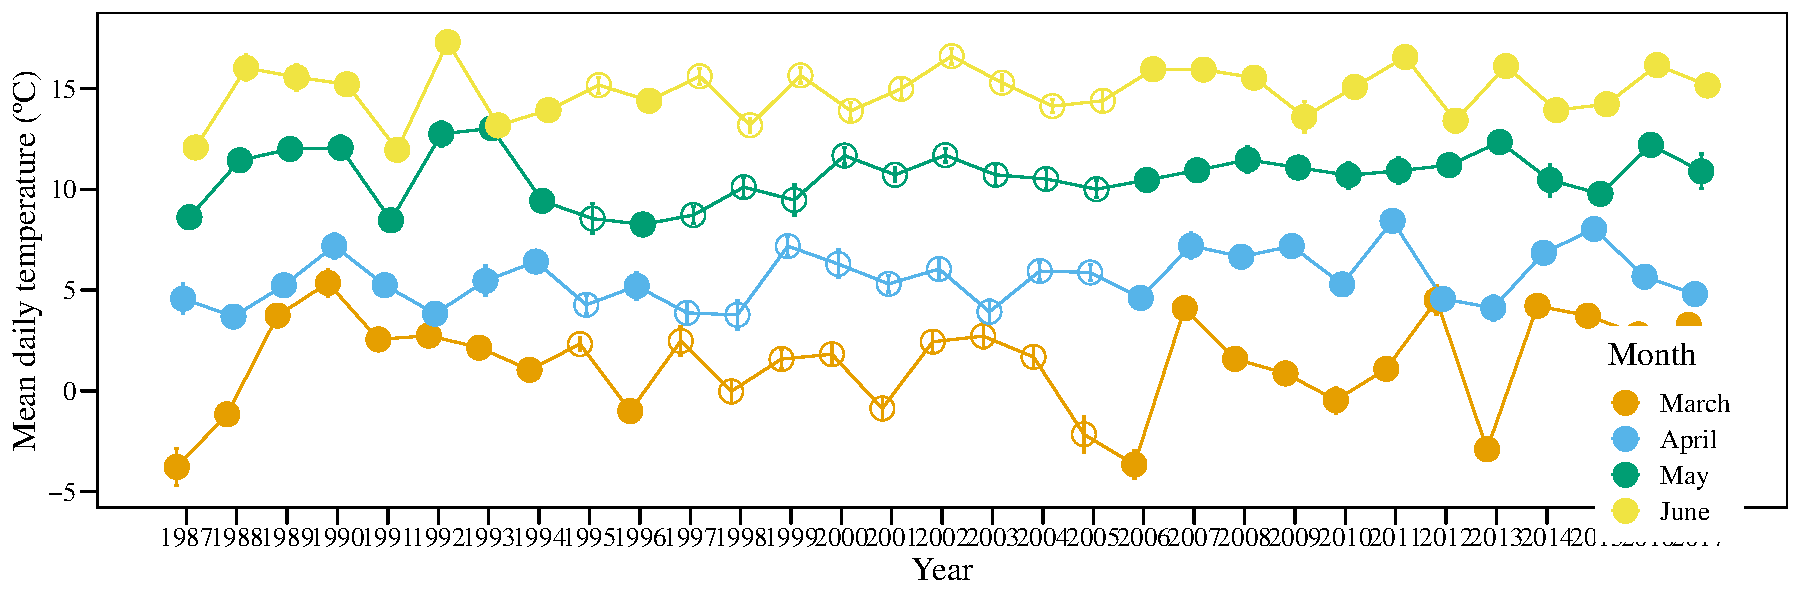
\includegraphics{lathyrus_ms3_3_after_rev_Ecology_files/figure-latex/unnamed-chunk-79-1.pdf}

\begin{Shaded}
\begin{Highlighting}[]
\KeywordTok{ggsave}\NormalTok{(}\DataTypeTok{filename=}\StringTok{"output/figures/AppendixS4.tiff"}\NormalTok{,}
       \DataTypeTok{device=}\StringTok{"tiff"}\NormalTok{,}\DataTypeTok{width=}\DecValTok{350}\NormalTok{,}\DataTypeTok{height=}\DecValTok{190}\NormalTok{,}\DataTypeTok{units=}\StringTok{"mm"}\NormalTok{,}\DataTypeTok{dpi=}\DecValTok{300}\NormalTok{,}\DataTypeTok{compression=}\StringTok{"lzw"}\NormalTok{)}
\end{Highlighting}
\end{Shaded}

\hypertarget{appendix-s5-relationships-fitness-ffd-for-each-level-of-mean-grazing-separately-for-each-year.}{%
\section{Appendix S5: Relationships fitness-FFD for each level of mean
grazing (separately for each
year).}\label{appendix-s5-relationships-fitness-ffd-for-each-level-of-mean-grazing-separately-for-each-year.}}

\begin{Shaded}
\begin{Highlighting}[]
\NormalTok{pred\_fitness\_all\textless{}{-}}\KeywordTok{ggpredict}\NormalTok{(mod\_int\_sel\_GLMM,}
                        \DataTypeTok{terms =} \KeywordTok{c}\NormalTok{(}\StringTok{"FFD\_s\_y [all]"}\NormalTok{,}\StringTok{"grazing\_mean [all]"}\NormalTok{))}
\NormalTok{data\_grazing\_cats\textless{}{-}}\KeywordTok{subset}\NormalTok{(data\_selag,}\OperatorTok{!}\KeywordTok{is.na}\NormalTok{(FFD\_s\_y)}\OperatorTok{\&!}\KeywordTok{is.na}\NormalTok{(fitness\_rel\_y))}\OperatorTok{\%\textgreater{}\%}
\StringTok{  }\KeywordTok{ungroup}\NormalTok{()}\OperatorTok{\%\textgreater{}\%}
\StringTok{  }\KeywordTok{select}\NormalTok{(}\StringTok{"year"}\NormalTok{,}\StringTok{"FFD\_s\_y"}\NormalTok{,}\StringTok{"fitness\_rel\_y"}\NormalTok{,}\StringTok{"grazing\_mean"}\NormalTok{)}\OperatorTok{\%\textgreater{}\%}
\StringTok{  }\KeywordTok{mutate}\NormalTok{(}\DataTypeTok{grazing\_mean=}\KeywordTok{round}\NormalTok{(grazing\_mean,}\DecValTok{3}\NormalTok{))}
\NormalTok{pred\_fitness\_all\_df\textless{}{-}}\KeywordTok{data.frame}\NormalTok{(pred\_fitness\_all)}\OperatorTok{\%\textgreater{}\%}
\StringTok{  }\NormalTok{dplyr}\OperatorTok{::}\KeywordTok{rename}\NormalTok{(}\DataTypeTok{FFD\_s\_y=}\NormalTok{x, }\DataTypeTok{fitness\_rel\_y=}\NormalTok{predicted,}\DataTypeTok{grazing\_mean=}\NormalTok{group)}\OperatorTok{\%\textgreater{}\%}
\StringTok{  }\KeywordTok{mutate}\NormalTok{(}\DataTypeTok{cat=}\StringTok{"prediction"}\NormalTok{,}
         \DataTypeTok{grazing\_mean=}\KeywordTok{as.numeric}\NormalTok{(}\KeywordTok{as.character}\NormalTok{(grazing\_mean)))}\OperatorTok{\%\textgreater{}\%}
\StringTok{  }\KeywordTok{left\_join}\NormalTok{(data\_grazing\_cats[}\KeywordTok{c}\NormalTok{(}\DecValTok{1}\NormalTok{,}\DecValTok{4}\NormalTok{)])}
\NormalTok{pred\_fitness\_byyear\textless{}{-}}
\StringTok{  }\KeywordTok{rbind}\NormalTok{(}
    \KeywordTok{data.frame}\NormalTok{(}\KeywordTok{ggpredict}\NormalTok{(mod\_int\_sel\_GLMM,}
                         \DataTypeTok{terms =} \KeywordTok{c}\NormalTok{(}\StringTok{"FFD\_s\_y [all]"}\NormalTok{,}\StringTok{"grazing\_mean [0.011]"}\NormalTok{)))}\OperatorTok{\%\textgreater{}\%}
\StringTok{      }\KeywordTok{mutate}\NormalTok{(}\DataTypeTok{year=}\DecValTok{1993}\NormalTok{)}\OperatorTok{\%\textgreater{}\%}
\StringTok{      }\NormalTok{dplyr}\OperatorTok{::}\KeywordTok{rename}\NormalTok{(}\DataTypeTok{FFD\_s\_y=}\NormalTok{x, }\DataTypeTok{fitness\_rel\_y=}\NormalTok{predicted,}\DataTypeTok{grazing\_mean=}\NormalTok{group),}
    \KeywordTok{data.frame}\NormalTok{(}\KeywordTok{ggpredict}\NormalTok{(mod\_int\_sel\_GLMM,}
                         \DataTypeTok{terms =} \KeywordTok{c}\NormalTok{(}\StringTok{"FFD\_s\_y [all]"}\NormalTok{,}\StringTok{"grazing\_mean [0.016]"}\NormalTok{)))}\OperatorTok{\%\textgreater{}\%}
\StringTok{      }\KeywordTok{mutate}\NormalTok{(}\DataTypeTok{year=}\DecValTok{1992}\NormalTok{)}\OperatorTok{\%\textgreater{}\%}
\StringTok{      }\NormalTok{dplyr}\OperatorTok{::}\KeywordTok{rename}\NormalTok{(}\DataTypeTok{FFD\_s\_y=}\NormalTok{x, }\DataTypeTok{fitness\_rel\_y=}\NormalTok{predicted,}\DataTypeTok{grazing\_mean=}\NormalTok{group),}
    \KeywordTok{data.frame}\NormalTok{(}\KeywordTok{ggpredict}\NormalTok{(mod\_int\_sel\_GLMM,}
                         \DataTypeTok{terms =} \KeywordTok{c}\NormalTok{(}\StringTok{"FFD\_s\_y [all]"}\NormalTok{,}\StringTok{"grazing\_mean [0.02]"}\NormalTok{)))}\OperatorTok{\%\textgreater{}\%}
\StringTok{      }\KeywordTok{mutate}\NormalTok{(}\DataTypeTok{year=}\DecValTok{2011}\NormalTok{)}\OperatorTok{\%\textgreater{}\%}
\StringTok{      }\NormalTok{dplyr}\OperatorTok{::}\KeywordTok{rename}\NormalTok{(}\DataTypeTok{FFD\_s\_y=}\NormalTok{x, }\DataTypeTok{fitness\_rel\_y=}\NormalTok{predicted,}\DataTypeTok{grazing\_mean=}\NormalTok{group),}
    \KeywordTok{data.frame}\NormalTok{(}\KeywordTok{ggpredict}\NormalTok{(mod\_int\_sel\_GLMM,}
                         \DataTypeTok{terms =} \KeywordTok{c}\NormalTok{(}\StringTok{"FFD\_s\_y [all]"}\NormalTok{,}\StringTok{"grazing\_mean [0.024]"}\NormalTok{)))}\OperatorTok{\%\textgreater{}\%}
\StringTok{      }\KeywordTok{mutate}\NormalTok{(}\DataTypeTok{year=}\DecValTok{2014}\NormalTok{)}\OperatorTok{\%\textgreater{}\%}
\StringTok{      }\NormalTok{dplyr}\OperatorTok{::}\KeywordTok{rename}\NormalTok{(}\DataTypeTok{FFD\_s\_y=}\NormalTok{x, }\DataTypeTok{fitness\_rel\_y=}\NormalTok{predicted,}\DataTypeTok{grazing\_mean=}\NormalTok{group),}
    \KeywordTok{data.frame}\NormalTok{(}\KeywordTok{ggpredict}\NormalTok{(mod\_int\_sel\_GLMM,}
                         \DataTypeTok{terms =} \KeywordTok{c}\NormalTok{(}\StringTok{"FFD\_s\_y [all]"}\NormalTok{,}\StringTok{"grazing\_mean [0.025]"}\NormalTok{)))}\OperatorTok{\%\textgreater{}\%}
\StringTok{      }\KeywordTok{mutate}\NormalTok{(}\DataTypeTok{year=}\DecValTok{2010}\NormalTok{)}\OperatorTok{\%\textgreater{}\%}
\StringTok{      }\NormalTok{dplyr}\OperatorTok{::}\KeywordTok{rename}\NormalTok{(}\DataTypeTok{FFD\_s\_y=}\NormalTok{x, }\DataTypeTok{fitness\_rel\_y=}\NormalTok{predicted,}\DataTypeTok{grazing\_mean=}\NormalTok{group),}
    \KeywordTok{data.frame}\NormalTok{(}\KeywordTok{ggpredict}\NormalTok{(mod\_int\_sel\_GLMM,}
                         \DataTypeTok{terms =} \KeywordTok{c}\NormalTok{(}\StringTok{"FFD\_s\_y [all]"}\NormalTok{,}\StringTok{"grazing\_mean [0.025]"}\NormalTok{)))}\OperatorTok{\%\textgreater{}\%}
\StringTok{      }\KeywordTok{mutate}\NormalTok{(}\DataTypeTok{year=}\DecValTok{2013}\NormalTok{)}\OperatorTok{\%\textgreater{}\%}
\StringTok{      }\NormalTok{dplyr}\OperatorTok{::}\KeywordTok{rename}\NormalTok{(}\DataTypeTok{FFD\_s\_y=}\NormalTok{x, }\DataTypeTok{fitness\_rel\_y=}\NormalTok{predicted,}\DataTypeTok{grazing\_mean=}\NormalTok{group),}
    \KeywordTok{data.frame}\NormalTok{(}\KeywordTok{ggpredict}\NormalTok{(mod\_int\_sel\_GLMM,}
                         \DataTypeTok{terms =} \KeywordTok{c}\NormalTok{(}\StringTok{"FFD\_s\_y [all]"}\NormalTok{,}\StringTok{"grazing\_mean [0.04]"}\NormalTok{)))}\OperatorTok{\%\textgreater{}\%}
\StringTok{      }\KeywordTok{mutate}\NormalTok{(}\DataTypeTok{year=}\DecValTok{1996}\NormalTok{)}\OperatorTok{\%\textgreater{}\%}
\StringTok{      }\NormalTok{dplyr}\OperatorTok{::}\KeywordTok{rename}\NormalTok{(}\DataTypeTok{FFD\_s\_y=}\NormalTok{x, }\DataTypeTok{fitness\_rel\_y=}\NormalTok{predicted,}\DataTypeTok{grazing\_mean=}\NormalTok{group),}
    \KeywordTok{data.frame}\NormalTok{(}\KeywordTok{ggpredict}\NormalTok{(mod\_int\_sel\_GLMM,}
                         \DataTypeTok{terms =} \KeywordTok{c}\NormalTok{(}\StringTok{"FFD\_s\_y [all]"}\NormalTok{,}\StringTok{"grazing\_mean [0.043]"}\NormalTok{)))}\OperatorTok{\%\textgreater{}\%}
\StringTok{      }\KeywordTok{mutate}\NormalTok{(}\DataTypeTok{year=}\DecValTok{1990}\NormalTok{)}\OperatorTok{\%\textgreater{}\%}
\StringTok{      }\NormalTok{dplyr}\OperatorTok{::}\KeywordTok{rename}\NormalTok{(}\DataTypeTok{FFD\_s\_y=}\NormalTok{x, }\DataTypeTok{fitness\_rel\_y=}\NormalTok{predicted,}\DataTypeTok{grazing\_mean=}\NormalTok{group),}
    \KeywordTok{data.frame}\NormalTok{(}\KeywordTok{ggpredict}\NormalTok{(mod\_int\_sel\_GLMM,}
                         \DataTypeTok{terms =} \KeywordTok{c}\NormalTok{(}\StringTok{"FFD\_s\_y [all]"}\NormalTok{,}\StringTok{"grazing\_mean [0.047]"}\NormalTok{)))}\OperatorTok{\%\textgreater{}\%}
\StringTok{      }\KeywordTok{mutate}\NormalTok{(}\DataTypeTok{year=}\DecValTok{1989}\NormalTok{)}\OperatorTok{\%\textgreater{}\%}
\StringTok{      }\NormalTok{dplyr}\OperatorTok{::}\KeywordTok{rename}\NormalTok{(}\DataTypeTok{FFD\_s\_y=}\NormalTok{x, }\DataTypeTok{fitness\_rel\_y=}\NormalTok{predicted,}\DataTypeTok{grazing\_mean=}\NormalTok{group),}
    \KeywordTok{data.frame}\NormalTok{(}\KeywordTok{ggpredict}\NormalTok{(mod\_int\_sel\_GLMM,}
                         \DataTypeTok{terms =} \KeywordTok{c}\NormalTok{(}\StringTok{"FFD\_s\_y [all]"}\NormalTok{,}\StringTok{"grazing\_mean [0.054]"}\NormalTok{)))}\OperatorTok{\%\textgreater{}\%}
\StringTok{      }\KeywordTok{mutate}\NormalTok{(}\DataTypeTok{year=}\DecValTok{1987}\NormalTok{)}\OperatorTok{\%\textgreater{}\%}
\StringTok{      }\NormalTok{dplyr}\OperatorTok{::}\KeywordTok{rename}\NormalTok{(}\DataTypeTok{FFD\_s\_y=}\NormalTok{x, }\DataTypeTok{fitness\_rel\_y=}\NormalTok{predicted,}\DataTypeTok{grazing\_mean=}\NormalTok{group),}
    \KeywordTok{data.frame}\NormalTok{(}\KeywordTok{ggpredict}\NormalTok{(mod\_int\_sel\_GLMM,}
                         \DataTypeTok{terms =} \KeywordTok{c}\NormalTok{(}\StringTok{"FFD\_s\_y [all]"}\NormalTok{,}\StringTok{"grazing\_mean [0.063]"}\NormalTok{)))}\OperatorTok{\%\textgreater{}\%}
\StringTok{      }\KeywordTok{mutate}\NormalTok{(}\DataTypeTok{year=}\DecValTok{2008}\NormalTok{)}\OperatorTok{\%\textgreater{}\%}
\StringTok{      }\NormalTok{dplyr}\OperatorTok{::}\KeywordTok{rename}\NormalTok{(}\DataTypeTok{FFD\_s\_y=}\NormalTok{x, }\DataTypeTok{fitness\_rel\_y=}\NormalTok{predicted,}\DataTypeTok{grazing\_mean=}\NormalTok{group),}
    \KeywordTok{data.frame}\NormalTok{(}\KeywordTok{ggpredict}\NormalTok{(mod\_int\_sel\_GLMM,}
                         \DataTypeTok{terms =} \KeywordTok{c}\NormalTok{(}\StringTok{"FFD\_s\_y [all]"}\NormalTok{,}\StringTok{"grazing\_mean [0.07]"}\NormalTok{)))}\OperatorTok{\%\textgreater{}\%}
\StringTok{      }\KeywordTok{mutate}\NormalTok{(}\DataTypeTok{year=}\DecValTok{1988}\NormalTok{)}\OperatorTok{\%\textgreater{}\%}
\StringTok{      }\NormalTok{dplyr}\OperatorTok{::}\KeywordTok{rename}\NormalTok{(}\DataTypeTok{FFD\_s\_y=}\NormalTok{x, }\DataTypeTok{fitness\_rel\_y=}\NormalTok{predicted,}\DataTypeTok{grazing\_mean=}\NormalTok{group),}
    \KeywordTok{data.frame}\NormalTok{(}\KeywordTok{ggpredict}\NormalTok{(mod\_int\_sel\_GLMM,}
                         \DataTypeTok{terms =} \KeywordTok{c}\NormalTok{(}\StringTok{"FFD\_s\_y [all]"}\NormalTok{,}\StringTok{"grazing\_mean [0.071]"}\NormalTok{)))}\OperatorTok{\%\textgreater{}\%}
\StringTok{      }\KeywordTok{mutate}\NormalTok{(}\DataTypeTok{year=}\DecValTok{2007}\NormalTok{)}\OperatorTok{\%\textgreater{}\%}
\StringTok{      }\NormalTok{dplyr}\OperatorTok{::}\KeywordTok{rename}\NormalTok{(}\DataTypeTok{FFD\_s\_y=}\NormalTok{x, }\DataTypeTok{fitness\_rel\_y=}\NormalTok{predicted,}\DataTypeTok{grazing\_mean=}\NormalTok{group),}
    \KeywordTok{data.frame}\NormalTok{(}\KeywordTok{ggpredict}\NormalTok{(mod\_int\_sel\_GLMM,}
                         \DataTypeTok{terms =} \KeywordTok{c}\NormalTok{(}\StringTok{"FFD\_s\_y [all]"}\NormalTok{,}\StringTok{"grazing\_mean [0.078]"}\NormalTok{)))}\OperatorTok{\%\textgreater{}\%}
\StringTok{      }\KeywordTok{mutate}\NormalTok{(}\DataTypeTok{year=}\DecValTok{2012}\NormalTok{)}\OperatorTok{\%\textgreater{}\%}
\StringTok{      }\NormalTok{dplyr}\OperatorTok{::}\KeywordTok{rename}\NormalTok{(}\DataTypeTok{FFD\_s\_y=}\NormalTok{x, }\DataTypeTok{fitness\_rel\_y=}\NormalTok{predicted,}\DataTypeTok{grazing\_mean=}\NormalTok{group),}
    \KeywordTok{data.frame}\NormalTok{(}\KeywordTok{ggpredict}\NormalTok{(mod\_int\_sel\_GLMM,}
                         \DataTypeTok{terms =} \KeywordTok{c}\NormalTok{(}\StringTok{"FFD\_s\_y [all]"}\NormalTok{,}\StringTok{"grazing\_mean [0.129]"}\NormalTok{)))}\OperatorTok{\%\textgreater{}\%}
\StringTok{      }\KeywordTok{mutate}\NormalTok{(}\DataTypeTok{year=}\DecValTok{2009}\NormalTok{)}\OperatorTok{\%\textgreater{}\%}
\StringTok{      }\NormalTok{dplyr}\OperatorTok{::}\KeywordTok{rename}\NormalTok{(}\DataTypeTok{FFD\_s\_y=}\NormalTok{x, }\DataTypeTok{fitness\_rel\_y=}\NormalTok{predicted,}\DataTypeTok{grazing\_mean=}\NormalTok{group),}
    \KeywordTok{data.frame}\NormalTok{(}\KeywordTok{ggpredict}\NormalTok{(mod\_int\_sel\_GLMM,}
                         \DataTypeTok{terms =} \KeywordTok{c}\NormalTok{(}\StringTok{"FFD\_s\_y [all]"}\NormalTok{,}\StringTok{"grazing\_mean [0.134]"}\NormalTok{)))}\OperatorTok{\%\textgreater{}\%}
\StringTok{      }\KeywordTok{mutate}\NormalTok{(}\DataTypeTok{year=}\DecValTok{1991}\NormalTok{)}\OperatorTok{\%\textgreater{}\%}
\StringTok{      }\NormalTok{dplyr}\OperatorTok{::}\KeywordTok{rename}\NormalTok{(}\DataTypeTok{FFD\_s\_y=}\NormalTok{x, }\DataTypeTok{fitness\_rel\_y=}\NormalTok{predicted,}\DataTypeTok{grazing\_mean=}\NormalTok{group),}
    \KeywordTok{data.frame}\NormalTok{(}\KeywordTok{ggpredict}\NormalTok{(mod\_int\_sel\_GLMM,}
                         \DataTypeTok{terms =} \KeywordTok{c}\NormalTok{(}\StringTok{"FFD\_s\_y [all]"}\NormalTok{,}\StringTok{"grazing\_mean [0.242]"}\NormalTok{)))}\OperatorTok{\%\textgreater{}\%}
\StringTok{      }\KeywordTok{mutate}\NormalTok{(}\DataTypeTok{year=}\DecValTok{2015}\NormalTok{)}\OperatorTok{\%\textgreater{}\%}
\StringTok{      }\NormalTok{dplyr}\OperatorTok{::}\KeywordTok{rename}\NormalTok{(}\DataTypeTok{FFD\_s\_y=}\NormalTok{x, }\DataTypeTok{fitness\_rel\_y=}\NormalTok{predicted,}\DataTypeTok{grazing\_mean=}\NormalTok{group),}
    \KeywordTok{data.frame}\NormalTok{(}\KeywordTok{ggpredict}\NormalTok{(mod\_int\_sel\_GLMM,}
                         \DataTypeTok{terms =} \KeywordTok{c}\NormalTok{(}\StringTok{"FFD\_s\_y [all]"}\NormalTok{,}\StringTok{"grazing\_mean [0.258]"}\NormalTok{)))}\OperatorTok{\%\textgreater{}\%}
\StringTok{      }\KeywordTok{mutate}\NormalTok{(}\DataTypeTok{year=}\DecValTok{2006}\NormalTok{)}\OperatorTok{\%\textgreater{}\%}
\StringTok{      }\NormalTok{dplyr}\OperatorTok{::}\KeywordTok{rename}\NormalTok{(}\DataTypeTok{FFD\_s\_y=}\NormalTok{x, }\DataTypeTok{fitness\_rel\_y=}\NormalTok{predicted,}\DataTypeTok{grazing\_mean=}\NormalTok{group),}
    \KeywordTok{data.frame}\NormalTok{(}\KeywordTok{ggpredict}\NormalTok{(mod\_int\_sel\_GLMM,}
                         \DataTypeTok{terms =} \KeywordTok{c}\NormalTok{(}\StringTok{"FFD\_s\_y [all]"}\NormalTok{,}\StringTok{"grazing\_mean [0.26]"}\NormalTok{)))}\OperatorTok{\%\textgreater{}\%}
\StringTok{      }\KeywordTok{mutate}\NormalTok{(}\DataTypeTok{year=}\DecValTok{2016}\NormalTok{)}\OperatorTok{\%\textgreater{}\%}
\StringTok{      }\NormalTok{dplyr}\OperatorTok{::}\KeywordTok{rename}\NormalTok{(}\DataTypeTok{FFD\_s\_y=}\NormalTok{x, }\DataTypeTok{fitness\_rel\_y=}\NormalTok{predicted,}\DataTypeTok{grazing\_mean=}\NormalTok{group),}
    \KeywordTok{data.frame}\NormalTok{(}\KeywordTok{ggpredict}\NormalTok{(mod\_int\_sel\_GLMM,}
                         \DataTypeTok{terms =} \KeywordTok{c}\NormalTok{(}\StringTok{"FFD\_s\_y [all]"}\NormalTok{,}\StringTok{"grazing\_mean [0.261]"}\NormalTok{)))}\OperatorTok{\%\textgreater{}\%}
\StringTok{      }\KeywordTok{mutate}\NormalTok{(}\DataTypeTok{year=}\DecValTok{1994}\NormalTok{)}\OperatorTok{\%\textgreater{}\%}
\StringTok{      }\NormalTok{dplyr}\OperatorTok{::}\KeywordTok{rename}\NormalTok{(}\DataTypeTok{FFD\_s\_y=}\NormalTok{x, }\DataTypeTok{fitness\_rel\_y=}\NormalTok{predicted,}\DataTypeTok{grazing\_mean=}\NormalTok{group),}
    \KeywordTok{data.frame}\NormalTok{(}\KeywordTok{ggpredict}\NormalTok{(mod\_int\_sel\_GLMM,}
                         \DataTypeTok{terms =} \KeywordTok{c}\NormalTok{(}\StringTok{"FFD\_s\_y [all]"}\NormalTok{,}\StringTok{"grazing\_mean [0.756]"}\NormalTok{)))}\OperatorTok{\%\textgreater{}\%}
\StringTok{      }\KeywordTok{mutate}\NormalTok{(}\DataTypeTok{year=}\DecValTok{2017}\NormalTok{)}\OperatorTok{\%\textgreater{}\%}
\StringTok{      }\NormalTok{dplyr}\OperatorTok{::}\KeywordTok{rename}\NormalTok{(}\DataTypeTok{FFD\_s\_y=}\NormalTok{x, }\DataTypeTok{fitness\_rel\_y=}\NormalTok{predicted,}\DataTypeTok{grazing\_mean=}\NormalTok{group)}
\NormalTok{  )}
\end{Highlighting}
\end{Shaded}

\begin{Shaded}
\begin{Highlighting}[]
\KeywordTok{ggplot}\NormalTok{(}\DataTypeTok{data=}\KeywordTok{subset}\NormalTok{(data\_grazing\_cats))}\OperatorTok{+}
\StringTok{  }\KeywordTok{geom\_jitter}\NormalTok{(}\KeywordTok{aes}\NormalTok{(}\DataTypeTok{x=}\NormalTok{FFD\_s\_y,}\DataTypeTok{y=}\NormalTok{fitness\_rel\_y),}\DataTypeTok{size=}\FloatTok{1.5}\NormalTok{,}\DataTypeTok{alpha=}\FloatTok{0.3}\NormalTok{,}\DataTypeTok{width=}\FloatTok{0.05}\NormalTok{)}\OperatorTok{+}
\StringTok{  }\KeywordTok{facet\_wrap\_paginate}\NormalTok{(}\OperatorTok{\textasciitilde{}}\NormalTok{grazing\_mean}\OperatorTok{+}\NormalTok{year,}\DataTypeTok{scales=}\StringTok{"free"}\NormalTok{,}\DataTypeTok{nrow=}\DecValTok{4}\NormalTok{,}\DataTypeTok{ncol=}\DecValTok{3}\NormalTok{,}\DataTypeTok{page=}\DecValTok{1}\NormalTok{,}
             \DataTypeTok{labeller =} \KeywordTok{labeller}\NormalTok{(label\_value,}\DataTypeTok{.multi\_line=}\NormalTok{F))}\OperatorTok{+}
\StringTok{  }\KeywordTok{geom\_line}\NormalTok{(}\DataTypeTok{data=}\NormalTok{pred\_fitness\_all\_df,}
            \KeywordTok{aes}\NormalTok{(FFD\_s\_y,fitness\_rel\_y,}
                \DataTypeTok{color=}\KeywordTok{as.numeric}\NormalTok{(}\KeywordTok{as.character}\NormalTok{(grazing\_mean))),}\DataTypeTok{size=}\DecValTok{1}\NormalTok{)}\OperatorTok{+}
\StringTok{  }\KeywordTok{geom\_ribbon}\NormalTok{(}\DataTypeTok{data=}\NormalTok{pred\_fitness\_byyear,}
            \KeywordTok{aes}\NormalTok{(}\DataTypeTok{x=}\NormalTok{FFD\_s\_y,}\DataTypeTok{y=}\NormalTok{fitness\_rel\_y,}\DataTypeTok{ymin=}\NormalTok{conf.low,}\DataTypeTok{ymax=}\NormalTok{conf.high,}
                \DataTypeTok{fill=}\KeywordTok{as.numeric}\NormalTok{(}\KeywordTok{as.character}\NormalTok{(grazing\_mean))),}\DataTypeTok{alpha=}\FloatTok{0.3}\NormalTok{)}\OperatorTok{+}
\StringTok{  }\KeywordTok{my\_theme}\NormalTok{()}\OperatorTok{+}\KeywordTok{scale\_color\_viridis}\NormalTok{(}\DataTypeTok{direction =} \DecValTok{{-}1}\NormalTok{)}\OperatorTok{+}
\StringTok{  }\KeywordTok{scale\_fill\_viridis}\NormalTok{(}\DataTypeTok{direction =} \DecValTok{{-}1}\NormalTok{)}\OperatorTok{+}
\StringTok{  }\KeywordTok{theme}\NormalTok{(}\DataTypeTok{legend.position=}\StringTok{"top"}\NormalTok{)}\OperatorTok{+}\KeywordTok{labs}\NormalTok{(}\DataTypeTok{colour=}\StringTok{"Mean grazing probability"}\NormalTok{)}\OperatorTok{+}
\StringTok{  }\KeywordTok{xlab}\NormalTok{(}\StringTok{"First flowering date"}\NormalTok{)}\OperatorTok{+}
\StringTok{  }\KeywordTok{ylab}\NormalTok{(}\StringTok{"Predicted fitness (number of intact seeds)"}\NormalTok{)}\OperatorTok{+}
\StringTok{  }\KeywordTok{theme}\NormalTok{(}\DataTypeTok{strip.text.x=}\KeywordTok{element\_text}\NormalTok{(}\DataTypeTok{margin=}\KeywordTok{margin}\NormalTok{(}\DecValTok{2}\NormalTok{,}\DecValTok{0}\NormalTok{,}\DecValTok{2}\NormalTok{,}\DecValTok{0}\NormalTok{)))}\OperatorTok{+}
\StringTok{  }\KeywordTok{guides}\NormalTok{(}\DataTypeTok{fill=}\OtherTok{FALSE}\NormalTok{)}
\end{Highlighting}
\end{Shaded}

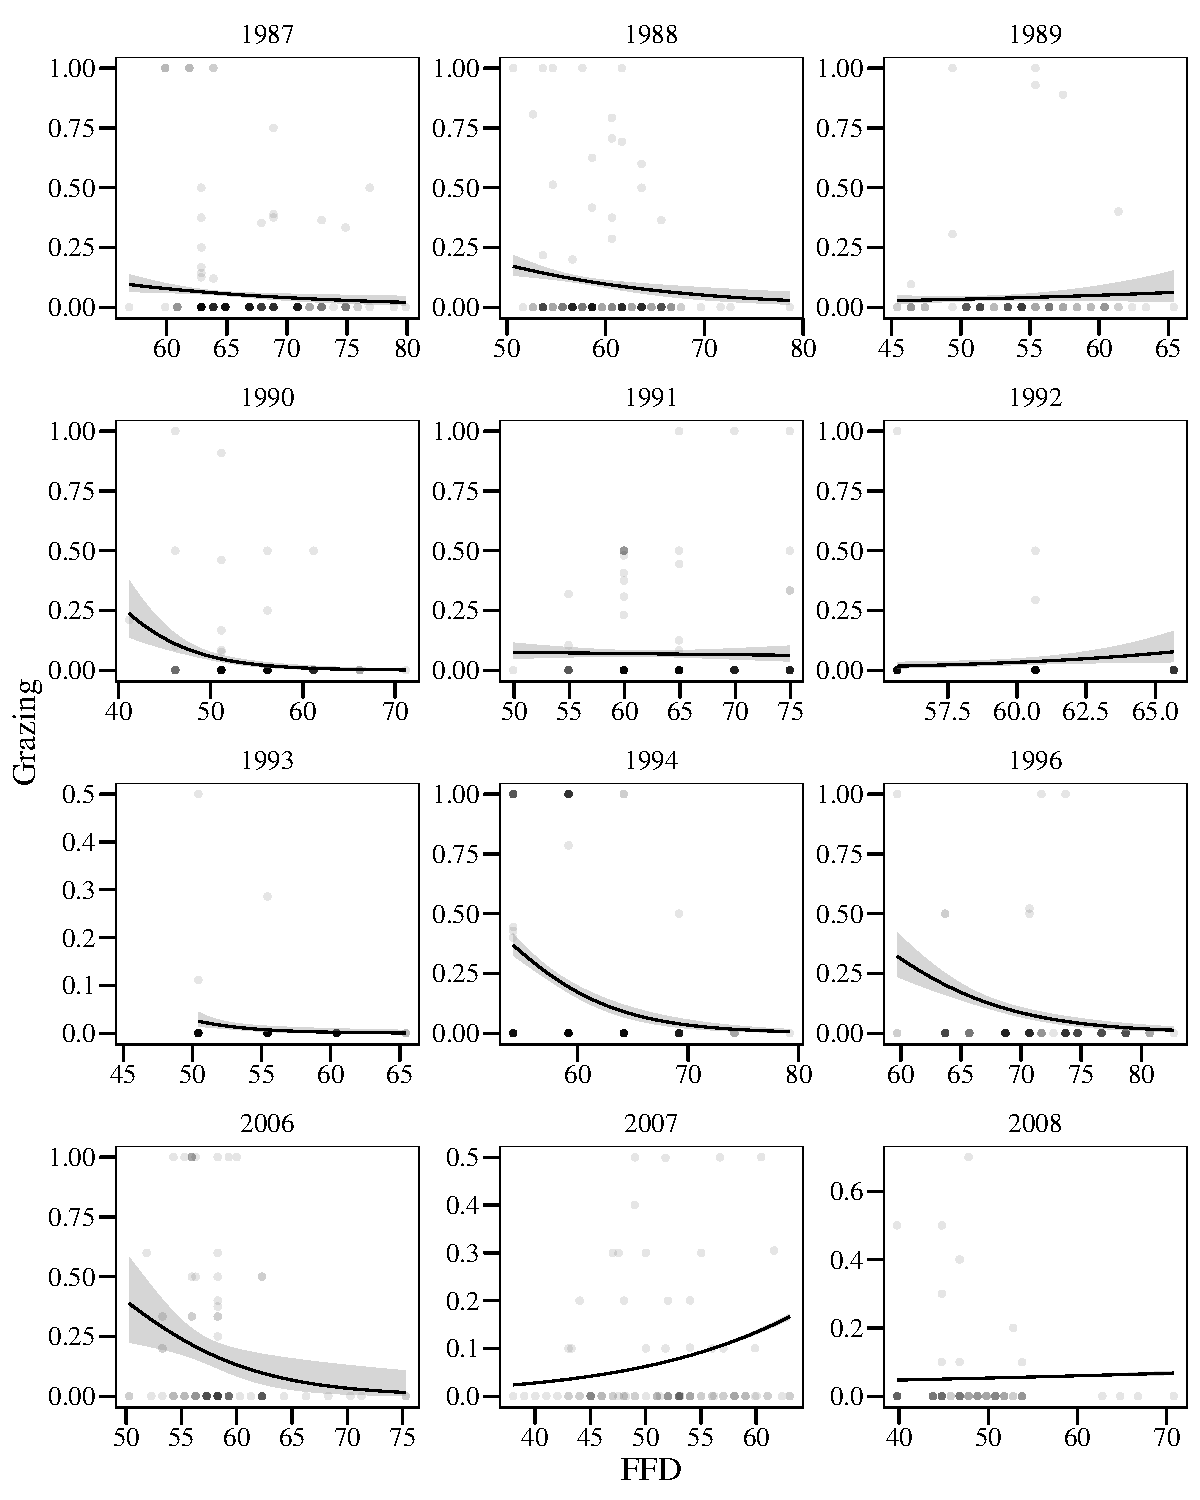
\includegraphics{lathyrus_ms3_3_after_rev_Ecology_files/figure-latex/unnamed-chunk-81-1.pdf}

\begin{Shaded}
\begin{Highlighting}[]
\KeywordTok{ggsave}\NormalTok{(}\DataTypeTok{filename=}\StringTok{"output/figures/AppendixS5\_A.tiff"}\NormalTok{,}\DataTypeTok{device=}\StringTok{"tiff"}\NormalTok{,}\DataTypeTok{width=}\DecValTok{168}\NormalTok{,}
       \DataTypeTok{height=}\DecValTok{210}\NormalTok{,}\DataTypeTok{units=}\StringTok{"mm"}\NormalTok{,}\DataTypeTok{dpi=}\DecValTok{300}\NormalTok{,}\DataTypeTok{compression=}\StringTok{"lzw"}\NormalTok{)}

\KeywordTok{ggplot}\NormalTok{(}\DataTypeTok{data=}\KeywordTok{subset}\NormalTok{(data\_grazing\_cats))}\OperatorTok{+}
\StringTok{  }\KeywordTok{geom\_jitter}\NormalTok{(}\KeywordTok{aes}\NormalTok{(}\DataTypeTok{x=}\NormalTok{FFD\_s\_y,}\DataTypeTok{y=}\NormalTok{fitness\_rel\_y),}\DataTypeTok{size=}\FloatTok{1.5}\NormalTok{,}\DataTypeTok{alpha=}\FloatTok{0.3}\NormalTok{,}\DataTypeTok{width=}\FloatTok{0.05}\NormalTok{)}\OperatorTok{+}
\StringTok{  }\KeywordTok{facet\_wrap\_paginate}\NormalTok{(}\OperatorTok{\textasciitilde{}}\NormalTok{grazing\_mean}\OperatorTok{+}\NormalTok{year,}\DataTypeTok{scales=}\StringTok{"free"}\NormalTok{,}\DataTypeTok{nrow=}\DecValTok{4}\NormalTok{,}\DataTypeTok{ncol=}\DecValTok{3}\NormalTok{,}\DataTypeTok{page=}\DecValTok{2}\NormalTok{,}
                      \DataTypeTok{labeller =} \KeywordTok{labeller}\NormalTok{(label\_value,}\DataTypeTok{.multi\_line=}\NormalTok{F))}\OperatorTok{+}
\StringTok{  }\KeywordTok{geom\_line}\NormalTok{(}\DataTypeTok{data=}\NormalTok{pred\_fitness\_all\_df,}
            \KeywordTok{aes}\NormalTok{(FFD\_s\_y,fitness\_rel\_y,}
                \DataTypeTok{color=}\KeywordTok{as.numeric}\NormalTok{(}\KeywordTok{as.character}\NormalTok{(grazing\_mean))),}\DataTypeTok{size=}\DecValTok{1}\NormalTok{)}\OperatorTok{+}
\StringTok{  }\KeywordTok{geom\_ribbon}\NormalTok{(}\DataTypeTok{data=}\NormalTok{pred\_fitness\_byyear,}
              \KeywordTok{aes}\NormalTok{(}\DataTypeTok{x=}\NormalTok{FFD\_s\_y,}\DataTypeTok{y=}\NormalTok{fitness\_rel\_y,}\DataTypeTok{ymin=}\NormalTok{conf.low,}\DataTypeTok{ymax=}\NormalTok{conf.high,}
                  \DataTypeTok{fill=}\KeywordTok{as.numeric}\NormalTok{(}\KeywordTok{as.character}\NormalTok{(grazing\_mean))),}\DataTypeTok{alpha=}\FloatTok{0.3}\NormalTok{)}\OperatorTok{+}
\StringTok{  }\KeywordTok{my\_theme}\NormalTok{()}\OperatorTok{+}\KeywordTok{scale\_color\_viridis}\NormalTok{(}\DataTypeTok{direction =} \DecValTok{{-}1}\NormalTok{)}\OperatorTok{+}
\StringTok{  }\KeywordTok{scale\_fill\_viridis}\NormalTok{(}\DataTypeTok{direction =} \DecValTok{{-}1}\NormalTok{)}\OperatorTok{+}
\StringTok{  }\KeywordTok{theme}\NormalTok{(}\DataTypeTok{legend.position=}\StringTok{"top"}\NormalTok{)}\OperatorTok{+}\KeywordTok{labs}\NormalTok{(}\DataTypeTok{colour=}\StringTok{"Mean grazing probability"}\NormalTok{)}\OperatorTok{+}
\StringTok{  }\KeywordTok{xlab}\NormalTok{(}\StringTok{"First flowering date"}\NormalTok{)}\OperatorTok{+}
\StringTok{  }\KeywordTok{ylab}\NormalTok{(}\StringTok{"Predicted fitness (number of intact seeds)"}\NormalTok{)}\OperatorTok{+}
\StringTok{  }\KeywordTok{theme}\NormalTok{(}\DataTypeTok{strip.text.x=}\KeywordTok{element\_text}\NormalTok{(}\DataTypeTok{margin=}\KeywordTok{margin}\NormalTok{(}\DecValTok{2}\NormalTok{,}\DecValTok{0}\NormalTok{,}\DecValTok{2}\NormalTok{,}\DecValTok{0}\NormalTok{)))}\OperatorTok{+}
\StringTok{  }\KeywordTok{guides}\NormalTok{(}\DataTypeTok{fill=}\OtherTok{FALSE}\NormalTok{)}
\end{Highlighting}
\end{Shaded}

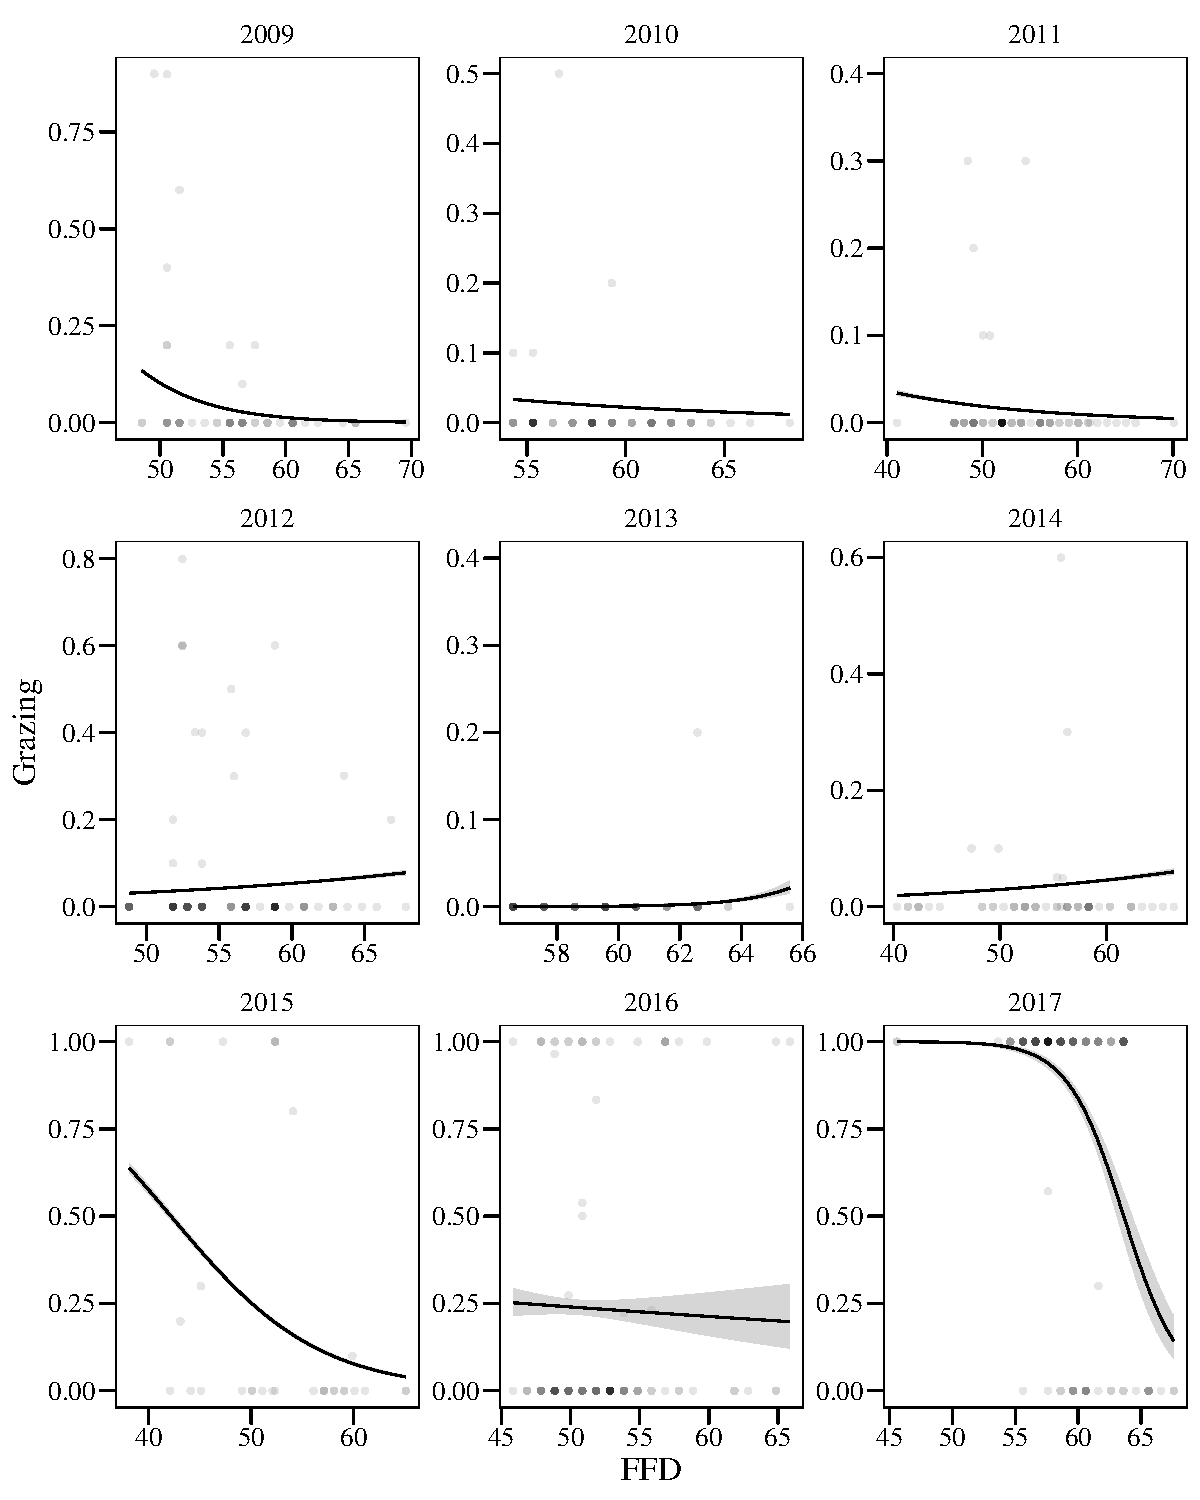
\includegraphics{lathyrus_ms3_3_after_rev_Ecology_files/figure-latex/unnamed-chunk-81-2.pdf}

\begin{Shaded}
\begin{Highlighting}[]
\KeywordTok{ggsave}\NormalTok{(}\DataTypeTok{filename=}\StringTok{"output/figures/AppendixS5\_B.tiff"}\NormalTok{,}\DataTypeTok{device=}\StringTok{"tiff"}\NormalTok{,}\DataTypeTok{width=}\DecValTok{168}\NormalTok{,}
       \DataTypeTok{height=}\DecValTok{210}\NormalTok{,}\DataTypeTok{units=}\StringTok{"mm"}\NormalTok{,}\DataTypeTok{dpi=}\DecValTok{300}\NormalTok{,}\DataTypeTok{compression=}\StringTok{"lzw"}\NormalTok{)}
\end{Highlighting}
\end{Shaded}

\hypertarget{appendix-x-relationship-between-flowering-frequency-and-ffd}{%
\section{Appendix X: Relationship between flowering frequency and
FFD}\label{appendix-x-relationship-between-flowering-frequency-and-ffd}}

\begin{Shaded}
\begin{Highlighting}[]
\CommentTok{\# fl\_freq=proportion of years that a plant flowered}
\CommentTok{\# (number of years flowering / number of years studied).}
\CommentTok{\# Using plants that were followed for 8{-}10 years (old period)}
\CommentTok{\# or 12  years (new period)}
\NormalTok{fl\_freq\textless{}{-}}\KeywordTok{read.table}\NormalTok{(}\StringTok{"data/fl\_freq.csv"}\NormalTok{,}\DataTypeTok{header=}\NormalTok{T,}\DataTypeTok{sep=}\StringTok{","}\NormalTok{,}\DataTypeTok{dec=}\StringTok{"."}\NormalTok{)}
\NormalTok{data\_fl\_freq\textless{}{-}data\_selag}\OperatorTok{\%\textgreater{}\%}
\StringTok{  }\KeywordTok{right\_join}\NormalTok{(fl\_freq[}\KeywordTok{c}\NormalTok{(}\DecValTok{3}\NormalTok{,}\DecValTok{6}\NormalTok{)])}\OperatorTok{\%\textgreater{}\%}
\StringTok{  }\KeywordTok{group\_by}\NormalTok{(id)}\OperatorTok{\%\textgreater{}\%}
\StringTok{  }\NormalTok{dplyr}\OperatorTok{::}\KeywordTok{summarise}\NormalTok{(}\DataTypeTok{mean\_FFD=}\KeywordTok{mean}\NormalTok{(FFD,}\DataTypeTok{na.rm=}\NormalTok{T),}\DataTypeTok{fl\_freq=}\KeywordTok{mean}\NormalTok{(fl\_freq))}
\KeywordTok{ggplot}\NormalTok{(data\_fl\_freq,}\KeywordTok{aes}\NormalTok{(}\DataTypeTok{x=}\NormalTok{fl\_freq,}\DataTypeTok{y=}\NormalTok{mean\_FFD))}\OperatorTok{+}
\StringTok{  }\KeywordTok{geom\_jitter}\NormalTok{(}\DataTypeTok{width=}\FloatTok{0.007}\NormalTok{,}\DataTypeTok{height=}\DecValTok{0}\NormalTok{,}\DataTypeTok{size=}\DecValTok{2}\NormalTok{,}\DataTypeTok{alpha=}\FloatTok{0.15}\NormalTok{)}\OperatorTok{+}
\StringTok{  }\KeywordTok{geom\_smooth}\NormalTok{(}\DataTypeTok{method=}\StringTok{"lm"}\NormalTok{,}\DataTypeTok{color=}\StringTok{"firebrick2"}\NormalTok{,}\DataTypeTok{fill=}\StringTok{"firebrick2"}\NormalTok{,}\DataTypeTok{size=}\DecValTok{1}\NormalTok{)}\OperatorTok{+}
\StringTok{  }\KeywordTok{xlab}\NormalTok{(}\StringTok{"Flowering frequency"}\NormalTok{)}\OperatorTok{+}\KeywordTok{ylab}\NormalTok{(}\StringTok{"Mean first flowering date"}\NormalTok{)}\OperatorTok{+}
\StringTok{  }\KeywordTok{my\_theme}\NormalTok{()}
\end{Highlighting}
\end{Shaded}

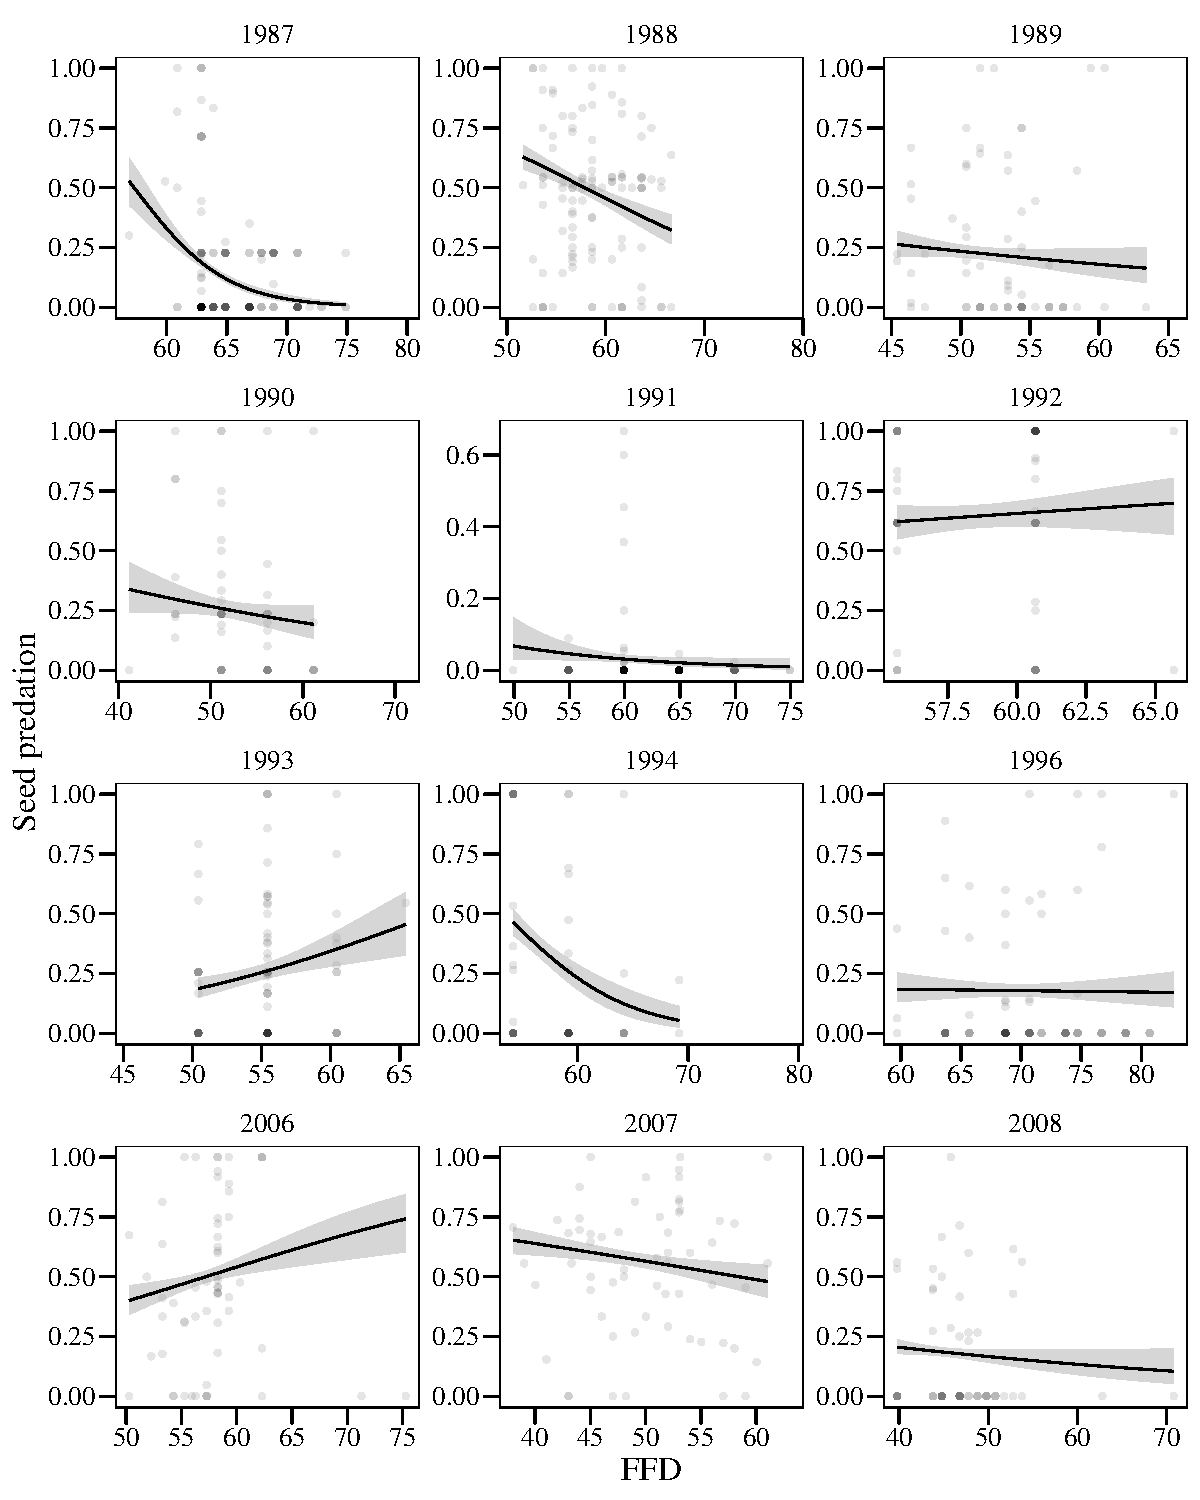
\includegraphics{lathyrus_ms3_3_after_rev_Ecology_files/figure-latex/unnamed-chunk-82-1.pdf}

\begin{Shaded}
\begin{Highlighting}[]
\CommentTok{\# Show this one}
\KeywordTok{ggsave}\NormalTok{(}\DataTypeTok{filename=}\StringTok{"output/figures/Appendix\_X.tiff"}\NormalTok{,}
       \DataTypeTok{device=}\StringTok{"tiff"}\NormalTok{,}\DataTypeTok{width=}\DecValTok{12}\NormalTok{,}\DataTypeTok{height=}\DecValTok{10}\NormalTok{,}\DataTypeTok{units=}\StringTok{"cm"}\NormalTok{,}\DataTypeTok{dpi=}\DecValTok{300}\NormalTok{,}\DataTypeTok{compression=}\StringTok{"lzw"}\NormalTok{)}
\KeywordTok{summary}\NormalTok{(}\KeywordTok{lm}\NormalTok{(mean\_FFD}\OperatorTok{\textasciitilde{}}\NormalTok{fl\_freq,}\DataTypeTok{data=}\NormalTok{data\_fl\_freq))}
\end{Highlighting}
\end{Shaded}

\begin{verbatim}
## 
## Call:
## lm(formula = mean_FFD ~ fl_freq, data = data_fl_freq)
## 
## Residuals:
##      Min       1Q   Median       3Q      Max 
## -19.3159  -3.5969   0.0362   3.2804  17.6316 
## 
## Coefficients:
##             Estimate Std. Error t value Pr(>|t|)    
## (Intercept)  61.8822     0.4060 152.412  < 2e-16 ***
## fl_freq      -5.6863     0.8247  -6.895 1.41e-11 ***
## ---
## Signif. codes:  0 '***' 0.001 '**' 0.01 '*' 0.05 '.' 0.1 ' ' 1
## 
## Residual standard error: 4.983 on 582 degrees of freedom
## Multiple R-squared:  0.07551,    Adjusted R-squared:  0.07393 
## F-statistic: 47.54 on 1 and 582 DF,  p-value: 1.408e-11
\end{verbatim}

\hypertarget{effects-of-variance-in-temperatures-on-interactions-not-used}{%
\section{Effects of variance in temperatures on interactions (not
used)}\label{effects-of-variance-in-temperatures-on-interactions-not-used}}

\begin{Shaded}
\begin{Highlighting}[]
\NormalTok{temp\_variance\textless{}{-}}\KeywordTok{read.table}\NormalTok{(}\StringTok{"data/temp\_variance.csv"}\NormalTok{,}
                          \DataTypeTok{header=}\NormalTok{T,}\DataTypeTok{sep=}\StringTok{"}\CharTok{\textbackslash{}t}\StringTok{"}\NormalTok{,}\DataTypeTok{dec=}\StringTok{"."}\NormalTok{) }
\NormalTok{data\_selag\textless{}{-}data\_selag}\OperatorTok{\%\textgreater{}\%}
\StringTok{  }\KeywordTok{left\_join}\NormalTok{(temp\_variance)}
\end{Highlighting}
\end{Shaded}

\begin{Shaded}
\begin{Highlighting}[]
\NormalTok{mod\_grazing\_tempvar\_bb\textless{}{-}}\KeywordTok{glmmTMB}\NormalTok{(}
  \KeywordTok{cbind}\NormalTok{(grazing\_success,grazing\_failure)}\OperatorTok{\textasciitilde{}}\KeywordTok{scale}\NormalTok{(var\_}\DecValTok{3}\NormalTok{)}\OperatorTok{+}\KeywordTok{scale}\NormalTok{(var\_}\DecValTok{4}\NormalTok{)}\OperatorTok{+}
\StringTok{    }\KeywordTok{scale}\NormalTok{(var\_}\DecValTok{5}\NormalTok{)}\OperatorTok{+}\NormalTok{FFD\_s\_y}\OperatorTok{+}\NormalTok{n\_fl\_s\_y}\OperatorTok{+}\NormalTok{(}\DecValTok{1}\OperatorTok{|}\NormalTok{id),}\DataTypeTok{data =}\NormalTok{ data\_selag,}
  \DataTypeTok{family=}\StringTok{"betabinomial"}\NormalTok{)}
\KeywordTok{summary}\NormalTok{(mod\_grazing\_tempvar\_bb)}
\end{Highlighting}
\end{Shaded}

\begin{verbatim}
##  Family: betabinomial  ( logit )
## Formula:          
## cbind(grazing_success, grazing_failure) ~ scale(var_3) + scale(var_4) +  
##     scale(var_5) + FFD_s_y + n_fl_s_y + (1 | id)
## Data: data_selag
## 
##      AIC      BIC   logLik deviance df.resid 
##   3886.1   3932.2  -1935.1   3870.1     2346 
## 
## Random effects:
## 
## Conditional model:
##  Groups Name        Variance Std.Dev.
##  id     (Intercept) 0.08705  0.295   
## Number of obs: 2354, groups:  id, 834
## 
## Overdispersion parameter for betabinomial family (): 0.144 
## 
## Conditional model:
##              Estimate Std. Error z value Pr(>|z|)    
## (Intercept)  -2.68741    0.10431 -25.764  < 2e-16 ***
## scale(var_3)  0.25612    0.06586   3.889 0.000101 ***
## scale(var_4) -0.37032    0.07318  -5.060 4.19e-07 ***
## scale(var_5)  0.49694    0.04092  12.145  < 2e-16 ***
## FFD_s_y      -0.27268    0.07340  -3.715 0.000203 ***
## n_fl_s_y      0.17445    0.05840   2.987 0.002814 ** 
## ---
## Signif. codes:  0 '***' 0.001 '**' 0.01 '*' 0.05 '.' 0.1 ' ' 1
\end{verbatim}

\begin{Shaded}
\begin{Highlighting}[]
\NormalTok{mod\_seedpred\_tempvar\_bb\textless{}{-}}\KeywordTok{glmmTMB}\NormalTok{(}
  \KeywordTok{cbind}\NormalTok{(}\KeywordTok{round}\NormalTok{(n\_pred\_seeds),}\KeywordTok{round}\NormalTok{(n\_intact\_seeds))}\OperatorTok{\textasciitilde{}}\StringTok{ }\KeywordTok{scale}\NormalTok{(var\_}\DecValTok{3}\NormalTok{)}\OperatorTok{+}\KeywordTok{scale}\NormalTok{(var\_}\DecValTok{4}\NormalTok{)}\OperatorTok{+}
\StringTok{    }\KeywordTok{scale}\NormalTok{(var\_}\DecValTok{5}\NormalTok{)}\OperatorTok{+}\KeywordTok{scale}\NormalTok{(var\_}\DecValTok{6}\NormalTok{)}\OperatorTok{+}\NormalTok{FFD\_s\_y}\OperatorTok{+}\NormalTok{n\_fl\_s\_y}\OperatorTok{+}\NormalTok{(}\DecValTok{1}\OperatorTok{|}\NormalTok{id),}\DataTypeTok{data =}\NormalTok{ data\_selag,}
  \DataTypeTok{family=}\StringTok{"betabinomial"}\NormalTok{)}
\KeywordTok{summary}\NormalTok{(mod\_seedpred\_tempvar\_bb)}
\end{Highlighting}
\end{Shaded}

\begin{verbatim}
##  Family: betabinomial  ( logit )
## Formula:          
## cbind(round(n_pred_seeds), round(n_intact_seeds)) ~ scale(var_3) +  
##     scale(var_4) + scale(var_5) + scale(var_6) + FFD_s_y + n_fl_s_y +  
##     (1 | id)
## Data: data_selag
## 
##      AIC      BIC   logLik deviance df.resid 
##   5415.9   5467.8  -2698.9   5397.9     2367 
## 
## Random effects:
## 
## Conditional model:
##  Groups Name        Variance Std.Dev.
##  id     (Intercept) 0.05261  0.2294  
## Number of obs: 2376, groups:  id, 834
## 
## Overdispersion parameter for betabinomial family (): 1.09 
## 
## Conditional model:
##              Estimate Std. Error z value Pr(>|z|)    
## (Intercept)  -1.03060    0.06321 -16.304  < 2e-16 ***
## scale(var_3)  0.20561    0.03954   5.200 1.99e-07 ***
## scale(var_4) -0.19578    0.05458  -3.587 0.000334 ***
## scale(var_5)  0.45494    0.05821   7.815 5.48e-15 ***
## scale(var_6)  0.36446    0.05041   7.230 4.82e-13 ***
## FFD_s_y       0.05971    0.05702   1.047 0.294982    
## n_fl_s_y      0.17777    0.04375   4.064 4.83e-05 ***
## ---
## Signif. codes:  0 '***' 0.001 '**' 0.01 '*' 0.05 '.' 0.1 ' ' 1
\end{verbatim}

Significant effects, but we probably do not want to get into this.

\hypertarget{period-effect}{%
\section{Period effect}\label{period-effect}}

\begin{Shaded}
\begin{Highlighting}[]
\NormalTok{mod\_grazing\_period\_bb\textless{}{-}}\KeywordTok{glmmTMB}\NormalTok{(}
  \KeywordTok{cbind}\NormalTok{(grazing\_success,grazing\_failure)}\OperatorTok{\textasciitilde{}}\KeywordTok{scale}\NormalTok{(mean\_}\DecValTok{3}\NormalTok{)}\OperatorTok{+}\KeywordTok{scale}\NormalTok{(mean\_}\DecValTok{4}\NormalTok{)}\OperatorTok{+}
\StringTok{    }\KeywordTok{scale}\NormalTok{(mean\_}\DecValTok{5}\NormalTok{)}\OperatorTok{+}\NormalTok{FFD\_s\_y}\OperatorTok{+}\NormalTok{n\_fl\_s\_y}\OperatorTok{+}\NormalTok{period}\OperatorTok{+}\NormalTok{(}\DecValTok{1}\OperatorTok{|}\NormalTok{id),}\DataTypeTok{data =}\NormalTok{ data\_selag,}
  \DataTypeTok{family=}\StringTok{"betabinomial"}\NormalTok{)}
\KeywordTok{summary}\NormalTok{(mod\_grazing\_period\_bb)}
\end{Highlighting}
\end{Shaded}

\begin{verbatim}
##  Family: betabinomial  ( logit )
## Formula:          
## cbind(grazing_success, grazing_failure) ~ scale(mean_3) + scale(mean_4) +  
##     scale(mean_5) + FFD_s_y + n_fl_s_y + period + (1 | id)
## Data: data_selag
## 
##      AIC      BIC   logLik deviance df.resid 
##   3929.7   3981.6  -1955.9   3911.7     2345 
## 
## Random effects:
## 
## Conditional model:
##  Groups Name        Variance Std.Dev.
##  id     (Intercept) 0.09705  0.3115  
## Number of obs: 2354, groups:  id, 834
## 
## Overdispersion parameter for betabinomial family (): 0.131 
## 
## Conditional model:
##               Estimate Std. Error z value Pr(>|z|)    
## (Intercept)   -1.51602    0.09468 -16.013  < 2e-16 ***
## scale(mean_3)  0.44493    0.06095   7.300 2.88e-13 ***
## scale(mean_4) -0.43953    0.06232  -7.053 1.75e-12 ***
## scale(mean_5) -0.69025    0.09749  -7.080 1.44e-12 ***
## FFD_s_y       -0.25386    0.07299  -3.478 0.000505 ***
## n_fl_s_y       0.18042    0.05904   3.056 0.002242 ** 
## periodold     -1.30087    0.15139  -8.593  < 2e-16 ***
## ---
## Signif. codes:  0 '***' 0.001 '**' 0.01 '*' 0.05 '.' 0.1 ' ' 1
\end{verbatim}

Significant period effect (disappears when removing 2017).

\begin{Shaded}
\begin{Highlighting}[]
\NormalTok{mod\_seedpred\_period\_bb\textless{}{-}}\KeywordTok{glmmTMB}\NormalTok{(}
  \KeywordTok{cbind}\NormalTok{(}\KeywordTok{round}\NormalTok{(n\_pred\_seeds),}\KeywordTok{round}\NormalTok{(n\_intact\_seeds))}\OperatorTok{\textasciitilde{}}\StringTok{ }\KeywordTok{scale}\NormalTok{(mean\_}\DecValTok{3}\NormalTok{)}\OperatorTok{+}\KeywordTok{scale}\NormalTok{(mean\_}\DecValTok{4}\NormalTok{)}\OperatorTok{+}
\StringTok{    }\KeywordTok{scale}\NormalTok{(mean\_}\DecValTok{5}\NormalTok{)}\OperatorTok{+}\KeywordTok{scale}\NormalTok{(mean\_}\DecValTok{6}\NormalTok{)}\OperatorTok{+}\NormalTok{FFD\_s\_y}\OperatorTok{+}\NormalTok{n\_fl\_s\_y}\OperatorTok{+}\NormalTok{period}\OperatorTok{+}\NormalTok{(}\DecValTok{1}\OperatorTok{|}\NormalTok{id),}\DataTypeTok{data =}\NormalTok{ data\_selag,}
  \DataTypeTok{family=}\StringTok{"betabinomial"}\NormalTok{)}
\KeywordTok{summary}\NormalTok{(mod\_seedpred\_period\_bb)}
\end{Highlighting}
\end{Shaded}

\begin{verbatim}
##  Family: betabinomial  ( logit )
## Formula:          
## cbind(round(n_pred_seeds), round(n_intact_seeds)) ~ scale(mean_3) +  
##     scale(mean_4) + scale(mean_5) + scale(mean_6) + FFD_s_y +  
##     n_fl_s_y + period + (1 | id)
## Data: data_selag
## 
##      AIC      BIC   logLik deviance df.resid 
##   5287.4   5345.1  -2633.7   5267.4     2366 
## 
## Random effects:
## 
## Conditional model:
##  Groups Name        Variance  Std.Dev. 
##  id     (Intercept) 3.708e-08 0.0001926
## Number of obs: 2376, groups:  id, 834
## 
## Overdispersion parameter for betabinomial family (): 1.15 
## 
## Conditional model:
##               Estimate Std. Error z value Pr(>|z|)    
## (Intercept)   -0.40840    0.08207  -4.976 6.47e-07 ***
## scale(mean_3) -0.16628    0.05378  -3.092  0.00199 ** 
## scale(mean_4) -0.08359    0.05083  -1.644  0.10011    
## scale(mean_5)  0.54418    0.08372   6.500 8.03e-11 ***
## scale(mean_6)  0.29881    0.05762   5.186 2.15e-07 ***
## FFD_s_y        0.02442    0.05590   0.437  0.66221    
## n_fl_s_y       0.18431    0.04337   4.250 2.14e-05 ***
## periodold     -0.81552    0.10662  -7.649 2.03e-14 ***
## ---
## Signif. codes:  0 '***' 0.001 '**' 0.01 '*' 0.05 '.' 0.1 ' ' 1
\end{verbatim}

\end{document}
